\let\origyear\year
%DIF LATEXDIFF DIFFERENCE FILE
%DIF DEL manuscript_submitted.tex   Sun Nov  1 13:09:21 2026
%DIF ADD manuscript.tex             Fri Nov 13 01:45:06 2026
\documentclass{ieeeaccess}
\let\IEEEaccessyear\year
\let\year\origyear
%Adjusted 05/13/2026 at the byline author names
%\usepackage[T1]{fontenc}
\usepackage{cite}
\bibliographystyle{IEEEtran}
\usepackage{amsmath,amssymb,amsfonts}
\usepackage{bm}
\usepackage{algorithm}
\usepackage{algpseudocode}
\usepackage{algorithmicx}
\usepackage{graphicx}
\graphicspath{{figures/}{./}}
\usepackage{tikz}
%DIF 17c17-19
%DIF < \usetikzlibrary{positioning, arrows.meta}
%DIF -------
\usetikzlibrary{positioning, arrows.meta, fit, calc} %DIF > 
\usepackage{pgfplots} %DIF > 
\pgfplotsset{compat=1.18} %DIF > 
%DIF -------
\definecolor{accessblue}{cmyk}{1,0.3,0,0.2}
\definecolor{greycolor}{cmyk}{0,0,0,0.8}
\definecolor{grey}{cmyk}{0,0,0,0.1}
\definecolor{black}{cmyk}{0,0,0,1}

% Architecture diagram palette
\definecolor{cMacro}{RGB}{20, 65, 115}
%DIF 25c27-31
%DIF < \definecolor{cMacroBg}{RGB}{242, 247, 253}
%DIF -------
\definecolor{cMacroBg}{RGB}{226, 236, 248} %DIF > 
% Series colors for Fig.~\ref{fig:budget} (validated for color-vision deficiency) %DIF > 
\definecolor{cSerA}{HTML}{2A78D6} %DIF > 
\definecolor{cSerB}{HTML}{EB6834} %DIF > 
\definecolor{cSerC}{HTML}{1BAF7A} %DIF > 
%DIF -------
\definecolor{cMicro}{RGB}{15, 95, 85}
\definecolor{cMicroBg}{RGB}{240, 249, 247}
\definecolor{cHeur}{RGB}{110, 25, 75}
\definecolor{cHeurBg}{RGB}{253, 242, 250}
\definecolor{cPool}{RGB}{165, 75, 10}
\definecolor{cPoolBg}{RGB}{255, 247, 238}
\definecolor{cMIP}{RGB}{125, 55, 15}
\definecolor{cMIPBg}{RGB}{252, 243, 236}
\definecolor{cArchive}{RGB}{20, 105, 50}
\definecolor{cArchiveBg}{RGB}{240, 250, 243}
\usepackage{textcomp}
\usepackage{booktabs}
\usepackage{tabularx}
\usepackage{multirow}
\usepackage{makecell}
\usepackage{balance}

\usepackage{hyperref}
\hypersetup{
    hidelinks,
    colorlinks=true,
    linkcolor=black,
    citecolor=black,
    urlcolor=black
}
\newcommand{\NV}{{N_\mathrm{V}}}
\newcommand{\TD}{{D_\mathrm{T}}}
%DIF 53a59-60
\newcommand{\NVs}[1]{N_{\mathrm{V},\text{#1}}} %DIF > 
\newcommand{\TDs}[1]{D_{\mathrm{T},\text{#1}}} %DIF > 
%DIF -------
\newcommand{\BKS}{\text{BKS}}
%DIF 54a62
\newcommand{\PENDING}[1]{\textbf{[PENDING: #1]}} %DIF > 
%DIF -------
\newdimen\xfigwd
\xfigwd=\textwidth

\makeatletter
\long\def\@makecaption#1#2{%
  \ifx\@captype\@IEEEtablestring
    \begin{flushleft}
    \vspace*{5pt}
    {\vss\color{accessblue}\tablecapheadfont #1. \ }{\raggedright\tablecapfont#2\vss}%
    \end{flushleft}
    \@IEEEtablecaptionsepspace
  \else
    \@IEEEfigurecaptionsepspace
    \setbox\@tempboxa\hbox{{\color{accessblue}\figcapheadfont #1. \ }}%
    \parbox[t]{\hsize}{\raggedright\noindent\unhbox\@tempboxa\figcapfont#2\strut}%
  \fi
}
\makeatother

\setlength{\textfloatsep}{5pt plus 1pt minus 1pt}
\setlength{\floatsep}{5pt plus 1pt minus 1pt}
\setlength{\intextsep}{5pt plus 1pt minus 1pt}
\setlength{\dbltextfloatsep}{3.5pt plus 1pt minus 1pt}
\setlength{\dblfloatsep}{5pt plus 1pt minus 1pt}

\newcommand{\BIBdecl}{\setlength{\itemsep}{-2.5pt}\setlength{\parsep}{0pt}}

\makeatletter
\def\@IEEEBIOskipN{0pt}
\AtBeginDocument{\DeclareMathVersion{bold}
\SetSymbolFont{operators}{bold}{T1}{times}{b}{n}
%\SetSymbolFont{NewLetters}{bold}{T1}{times}{b}{it}
\SetMathAlphabet{\mathrm}{bold}{T1}{times}{b}{n}
\SetMathAlphabet{\mathit}{bold}{T1}{times}{b}{it}
\SetMathAlphabet{\mathbf}{bold}{T1}{times}{b}{n}
\SetMathAlphabet{\mathtt}{bold}{OT1}{pcr}{b}{n}
\SetSymbolFont{symbols}{bold}{OMS}{cmsy}{b}{n}
\renewcommand\boldmath{\@nomath\boldmath\mathversion{bold}}}
\makeatother

\def\BibTeX{{\rm B\kern-.05em{\sc i\kern-.025em b}\kern-.08em
    T\kern-.1667em\lower.7ex\hbox{E}\kern-.125emX}}



\makeatletter
\ifx\@biographyTOCentrynotmade\@undefined
  \newif\if@biographyTOCentrynotmade
  \@biographyTOCentrynotmadetrue
\fi
\@ifundefined{c@biography}{\newcounter{biography}}{}
\makeatother


\makeatletter
\renewenvironment{IEEEbiography}[2][]{%
    \normalfont\biographyfont%
    \unitlength 1in%
    \parskip=0pt%
    \par%
    \parindent 1em%
    \interlinepenalty 500%
    \@IEEEtranneedspace{\@IEEEBIOhangdepth}{\relax}%
    \vskip 0pt%
    \def\@IEEEtempbiographybox{%
        \mbox{%
            \begin{minipage}[b][\@IEEEBIOphotodepth][c]%
            {\@IEEEBIOphotowidth}%
            \centering
            PLACE PHOTO HERE
            \end{minipage}%
        }%
    }%
    \@ifmtarg{#1}{\relax}{%
        \def\@IEEEtempbiographybox{%
            \mbox{%
                \begin{minipage}[b][\@IEEEBIOphotodepth][c]%
                {\@IEEEBIOphotowidth}%
                \centering
                #1%
                \end{minipage}%
            }%
        }%
    }%
    \hangindent\@IEEEBIOhangwidth%
    \hangafter-\@IEEEtrantmpcountA%
    \settoheight{\@IEEEtrantmpdimenB}{\mbox{T}}%
    \noindent
    \makebox[0pt][l]{%
        \hspace{-\@IEEEBIOhangwidth}%
        \raisebox{\@IEEEtrantmpdimenB}[0pt][0pt]{%
            \raisebox{-\@IEEEBIOphotodepth}[0pt][0pt]{%
                \@IEEEtempbiographybox
            }%
        }%
    }%
    \noindent
    {\biographyheadfont\uppercase{#2}\ }%
    \@IEEEgobbleleadPARNLSP
}{%
    \relax
    \par
    \normalfont
    \vspace{6em}% <-- increase/decrease distance here
}
\makeatother

%Your document starts from here ___________________________________________________
%DIF PREAMBLE EXTENSION ADDED BY LATEXDIFF
%DIF UNDERLINE PREAMBLE %DIF PREAMBLE
\RequirePackage[normalem]{ulem} %DIF PREAMBLE
\RequirePackage{color}\definecolor{RED}{rgb}{1,0,0}\definecolor{BLUE}{rgb}{0,0,1} %DIF PREAMBLE
\newcommand{\DIFaddhl}[1]{\bgroup\markoverwith{\textcolor{yellow}{\rule[-.6ex]{2pt}{2.6ex}}}\ULon{#1}} %DIF PREAMBLE
\newcommand{\DIFaddmath}[1]{{\color{blue}#1}} %DIF PREAMBLE
\providecommand{\DIFaddtex}[1]{{\protect\color{blue}\uwave{#1}}} %DIF PREAMBLE
\providecommand{\DIFdeltex}[1]{{\protect\color{red}\sout{#1}}} %DIF PREAMBLE
%DIF SAFE PREAMBLE %DIF PREAMBLE
\providecommand{\DIFaddbegin}{} %DIF PREAMBLE
\providecommand{\DIFaddend}{} %DIF PREAMBLE
\providecommand{\DIFdelbegin}{} %DIF PREAMBLE
\providecommand{\DIFdelend}{} %DIF PREAMBLE
\providecommand{\DIFmodbegin}{} %DIF PREAMBLE
\providecommand{\DIFmodend}{} %DIF PREAMBLE
%DIF FLOATSAFE PREAMBLE %DIF PREAMBLE
\DeclareRobustCommand{\DIFaddFL}[1]{\ifmmode\expandafter\DIFaddmath\else\expandafter\DIFaddhl\fi{#1}} %DIF PREAMBLE
\providecommand{\DIFdelFL}[1]{\DIFdel{#1}} %DIF PREAMBLE
\providecommand{\DIFaddbeginFL}{} %DIF PREAMBLE
\providecommand{\DIFaddendFL}{} %DIF PREAMBLE
\providecommand{\DIFdelbeginFL}{} %DIF PREAMBLE
\providecommand{\DIFdelendFL}{} %DIF PREAMBLE
%DIF HYPERREF PREAMBLE %DIF PREAMBLE
\DeclareRobustCommand{\DIFadd}[1]{\ifmmode\expandafter\DIFaddmath\else\expandafter\DIFaddhl\fi{#1}} %DIF PREAMBLE
\providecommand{\DIFdel}[1]{\texorpdfstring{\DIFdeltex{#1}}{}} %DIF PREAMBLE
%DIF AMSMATHULEM PREAMBLE %DIF PREAMBLE
\makeatletter %DIF PREAMBLE
\let\sout@orig\sout %DIF PREAMBLE
\renewcommand{\sout}[1]{\ifmmode\text{\sout@orig{\ensuremath{#1}}}\else\sout@orig{#1}\fi} %DIF PREAMBLE
\makeatother %DIF PREAMBLE
%DIF COLORLISTINGS PREAMBLE %DIF PREAMBLE
\RequirePackage{listings} %DIF PREAMBLE
\RequirePackage{color} %DIF PREAMBLE
\lstdefinelanguage{DIFcode}{ %DIF PREAMBLE
%DIF DIFCODE_UNDERLINE %DIF PREAMBLE
  moredelim=[il][\color{red}\sout]{\%DIF\ <\ }, %DIF PREAMBLE
  moredelim=[il][\color{blue}\uwave]{\%DIF\ >\ } %DIF PREAMBLE
} %DIF PREAMBLE
\lstdefinestyle{DIFverbatimstyle}{ %DIF PREAMBLE
	language=DIFcode, %DIF PREAMBLE
	basicstyle=\ttfamily, %DIF PREAMBLE
	columns=fullflexible, %DIF PREAMBLE
	keepspaces=true %DIF PREAMBLE
} %DIF PREAMBLE
\lstnewenvironment{DIFverbatim}[1][]{\lstset{style=DIFverbatimstyle}}{} %DIF PREAMBLE
\lstnewenvironment{DIFverbatim*}[1][]{\lstset{style=DIFverbatimstyle,showspaces=true}}{} %DIF PREAMBLE
\lstset{extendedchars=\true,inputencoding=utf8}

%DIF END PREAMBLE EXTENSION ADDED BY LATEXDIFF

\begin{document}
\history{Date of publication xxxx 00, 0000, date of current version xxxx 00, 0000.}
\doi{10.1109/ACCESS.2026.DOI}

\title{Tri-Level Hybrid DDQN-ALNS: A Hierarchical Learning-Augmented Metaheuristic for the Vehicle Routing Problem with Time Windows}

\author{\uppercase{Huynh Nhat Huy}\authorrefmark{1}, \uppercase{Thi-Linh Ho}\authorrefmark{2}, \uppercase{Nguyen Nhat Huy}\authorrefmark{3}, \uppercase{and Nguyen Thi Bao Tran}\authorrefmark{4}}

\address[1]{Faculty of Information Technology, Ton Duc Thang University, Ho Chi Minh City, Vietnam (e-mail: huynhnthuy@tdtu.edu.vn)}
\address[2]{Natural Language Processing and Knowledge Discovery Research Group, Faculty of Information Technology, Ton Duc Thang University, Ho Chi Minh City, Vietnam (e-mail: hothilinh@tdtu.edu.vn)}
\address[3]{Mindx, Ho Chi Minh City, Vietnam (e-mail: huynguyenwork14@gmail.com)}
\address[4]{Vinsmart future, Ho Chi Minh City, Vietnam (e-mail: tranntb.se@gmail.com)}

\tfootnote{This research is supported by Ton Duc Thang University.}

%\markboth
%{Huy \headeretal: Tri-Level Hybrid DDQN-ALNS for VRPTW}
%{Huy \headeretal: Tri-Level Hybrid DDQN-ALNS for VRPTW}

\corresp{Corresponding author: Thi-Linh Ho (e-mail: hothilinh@tdtu.edu.vn).}

\newlength{\realabstractwidth}
\setlength{\realabstractwidth}{\titlewidth}
\addtolength{\realabstractwidth}{-9.27pt}
\let\abstractwidth\realabstractwidth
\DIFaddbegin 

\DIFaddend \begin{abstract}
The Vehicle Routing Problem with Time Windows (VRPTW) is  \DIFaddbegin \DIFadd{commonly solved under a lexicographic objective: minimize the number of }\DIFaddend vehicles ($\NV$)  \DIFaddbegin \DIFadd{first, then }\DIFaddend total travel distance ($\TD$).  \DIFaddbegin \DIFadd{We ask whether learned control inside }\DIFaddend Adaptive Large Neighborhood Search (ALNS)  \DIFaddbegin \DIFadd{pays for its compute when the controllers start from random weights in every run. The test case, }\DIFaddend Tri-Level Hybrid DDQN-ALNS, \DIFaddbegin \DIFadd{adds three online-learning controllers to ALNS: }\DIFaddend a  \DIFaddbegin \DIFadd{macro plateau controller, }\DIFaddend a \DIFaddbegin \DIFadd{micro operator controller built on a }\DIFaddend Dueling Double Deep Q-Network \DIFaddbegin \DIFadd{, and }\DIFaddend a Learned Acceptance Criterion  \DIFaddbegin \DIFadd{that can accept moves Simulated Annealing rejects. The search also uses ejection chains, set partitioning with HiGHS, a frozen }\DIFaddend Graph Neural Network  \DIFaddbegin \DIFadd{edge heatmap, and a classical Guided Ejection Search phase. That phase was added after earlier benchmark results were seen and kept by a pre-specified rule, so its inclusion was not independently tested. We claim neither a new search principle nor a convergence guarantee. We evaluate the method under equal wall-clock budgets of 10, 60 }\DIFaddend and  \DIFaddbegin \DIFadd{300\,s on 74 Solomon and Gehring-Homberger instances with five seeds per instance, against ALNS-Base, PyVRP-ILS and NeuroLKH-adapted, counting only incumbents certified in the original problem space before the cutoff. At 300\,s, the proposed configuration did not differ detectably on fleet size (fleet score, 98.33\% interval; positive favors it) from ALNS-Base ($-0.027$ }[\DIFadd{$-0.065$, $0.011$}]\DIFadd{), PyVRP-ILS ($+0.008$ }[\DIFadd{$-0.098$, $0.117$}]\DIFadd{) or NeuroLKH-adapted ($-0.068$ }[\DIFadd{$-0.142$, $0.033$}]\DIFadd{). In a factorial ablation on 18 instances, no primary factorial contrast's fleet-score interval excluded zero at 300\,s.
}\DIFaddend \end{abstract}

\begin{keywords}
Adaptive Large Neighborhood Search, Deep Reinforcement Learning, Double DQN, Semi-Markov Decision Process, Metaheuristics, Vehicle Routing Problem with Time Windows.
\end{keywords}

\titlepgskip=-19.5pt

\maketitle

\section{Introduction}
\label{sec:introduction}

\PARstart{T}{he} Vehicle Routing Problem with Time Windows (VRPTW) is  \DIFaddbegin \DIFadd{an }\DIFaddend NP-hard combinatorial optimization problem  \DIFaddbegin \DIFadd{that arises in freight logistics and }\DIFaddend last-mile parcel delivery  \DIFaddbegin \DIFadd{\mbox{%DIFAUXCMD
\cite{Dantzig1959, Solomon1987}}\hskip0pt%DIFAUXCMD
. Each route must }\DIFaddend respect vehicle capacity  \DIFaddbegin \DIFadd{and the time window of every customer it visits}\DIFaddend .

 \DIFaddbegin \DIFadd{Commercial freight planning often treats the objective as }\DIFaddend lexicographic: dispatchers prioritize minimizing the total number of deployed vehicles ($\NV$) before minimizing total travel distance ($\TD$) \cite{Toth2014, braysy2005vehicle}. Formally, letting $\mathcal{S}$ denote the space of feasible routing solutions, a solution $s_1 \in \mathcal{S}$ is strictly preferred over $s_2 \in \mathcal{S}$ (denoted $s_1 \prec s_2$) if and only if:
 \DIFaddbegin \begin{equation}
  \DIFadd{\begin{aligned}
    \NV(s_1) < \NV(s_2) \;\lor\; \big(&\NV(s_1) = \NV(s_2) \;\land \\
    &\TD(s_1) < \TD(s_2)\big)
  \end{aligned}
  \label{eq:lexicographic_intro}
}\end{equation}\DIFaddend 
This  ordering reflects the  \DIFaddbegin \DIFadd{cost }\DIFaddend structure of commercial  \DIFaddbegin \DIFadd{transport, where vehicle }\DIFaddend acquisition, maintenance, insurance  \DIFaddbegin \DIFadd{and driver wages outweigh marginal fuel cost}\DIFaddend .

Adaptive Large Neighborhood Search (ALNS) \cite{pisinger2007general, Ropke2006}  \DIFaddbegin \DIFadd{is }\DIFaddend a leading metaheuristic  \DIFaddbegin \DIFadd{for VRPTW. It repeatedly destroys and repairs parts of a solution, and its standard form keeps solutions feasible. Standard implementations choose operators with }\DIFaddend roulette-wheel or  \DIFaddbegin \DIFadd{bandit rules that aggregate reward scores over }\DIFaddend coarse segments.  \DIFaddbegin \DIFadd{These rules do not condition on the current search state, such as }\DIFaddend route fragmentation, temporal slack  \DIFaddbegin \DIFadd{or capacity use, and they do not coordinate the several steps needed to leave a plateau on which removing a vehicle means passing through worse intermediate solutions. Learned controllers that condition these choices on the search state have been proposed \mbox{%DIFAUXCMD
\cite{kallestad2023general, johnn2023graph, reijnen2024online}}\hskip0pt%DIFAUXCMD
. They are not free: every network update and every forward pass takes time from the search itself, so under a fixed wall-clock budget a learned controller must gain more than it costs.
}\DIFaddend 

 Neural Combinatorial Optimization (NCO)  \DIFaddbegin \DIFadd{takes a different approach and learns to construct routes end to end, with }\DIFaddend Pointer Networks \cite{vinyals2015pointer}, Attention Models \cite{kool2019attention}  and constructive policies \cite{nazari2018reinforcement}.  \DIFaddbegin \DIFadd{Such models are usually trained to minimize distance, and hard time windows complicate autoregressive decoding \mbox{%DIFAUXCMD
\cite{falkner2020learning, lin2021deep}}\hskip0pt%DIFAUXCMD
. We do not evaluate }\DIFaddend end-to-end  \DIFaddbegin \DIFadd{solvers here; we study the other option, learning inside a search that already handles the constraints.
}\DIFaddend 

 \DIFaddbegin \DIFadd{This paper asks whether learned control inside ALNS pays for its compute when the controllers start from random weights in every run. The test case is }\DIFaddend Tri-Level Hybrid DDQN-ALNS,  \DIFaddbegin \DIFadd{which places }\DIFaddend state-conditioned reinforcement learning  \DIFaddbegin \DIFadd{inside the }\DIFaddend search loop of ALNS \DIFaddbegin \DIFadd{, keeps the ALNS neighborhood operators and returns only solutions validated as feasible. The search has three tiers: a learned macro controller for plateaus, a learned micro controller for operator selection, and a heuristic search tier. At 300\,s our answer is negative: the method did not differ detectably on fleet size from ALNS-Base, PyVRP-ILS or NeuroLKH-adapted, and the factorial ablation does not establish a benefit of the learned components at that budget. The ablation is also less informative than it looks: in a separate measurement at 300\,s the acceptance model never changed an acceptance decision and the macro controller made no decision on the R2 and RC2 instances, so parts of the learned layer were hardly exercised. The one signal for learning is at 60\,s: in a separate test on new time-window variants, Micro-DDQN used fewer vehicles than a rule-based policy in the bare configuration, and the test did not detect a difference in the full context (Section~\ref{sec:ablation_results}).
}\DIFaddend 

The primary contributions of this paper are summarized as follows:
\begin{enumerate}\setlength{\itemsep}{0pt}\setlength{\parskip}{0pt}
    \item We  \DIFaddbegin \DIFadd{specify a control layer for ALNS in which a macro plateau controller, a micro operator controller and an acceptance model learn online from random weights in every run, with no offline policy training. Destroy-repair search, Simulated Annealing, ejection chains and set partitioning are established methods, and we do not claim a new search principle. What we study is whether such cold-start control pays for its compute within a time budget.
    }\DIFaddend \item  We evaluate the  \DIFaddbegin \DIFadd{method under equal wall-clock budgets of 10, 60 and 300\,s on }\DIFaddend 74  benchmark instances (56 Solomon-100, 12 Homberger-200, and 6 Homberger-400)  \DIFaddbegin \DIFadd{with five seeds, against ALNS-Base, PyVRP-ILS }\DIFaddend and  \DIFaddbegin \DIFadd{NeuroLKH-adapted. All cases of an instance, seed and cutoff run as one block, and only incumbents certified in the original problem space before the cutoff count. At 300\,s, the method did not differ detectably on fleet size from any of the three comparators, and we report this as a negative result.
    }\item \DIFadd{We separate learning from heuristic machinery with a wall-clock factorial ablation over six components at 60 and 300\,s, including a $2\times2$ contrast of the learning and heuristic bundles. The Guided Ejection Search phase is on in every case, so the ablation cannot isolate its effect. No primary contrast excluded zero at 300\,s. In a separate measurement on the ablation instances, the LAC classifier never changed an acceptance decision at that budget, so the LAC contrast is uninformative rather than evidence that LAC has no effect.
    }\item \DIFadd{We report the limits of the method and of the evidence: where it does not help, how results depend on the budget, the method's earlier dependence on reference fleet sizes, the machine-speed variation we measured, and the way test results influenced development}\DIFaddend .
\end{enumerate}

The remainder of this paper is organized as follows: Section~\ref{sec:related_work} reviews related literature. Section~\ref{sec:formulation} presents the problem formulation. Section~\ref{sec:methodology} describes the  \DIFaddbegin \DIFadd{method}\DIFaddend . Section~\ref{sec:experiments}  \DIFaddbegin \DIFadd{reports the }\DIFaddend benchmark results, statistical  \DIFaddbegin \DIFadd{analysis and ablation}\DIFaddend . Section~\ref{sec:discussion} discusses  \DIFaddbegin \DIFadd{where the method does and does not help, its practical meaning, and its }\DIFaddend limitations. Finally, Section~\ref{sec:conclusion} concludes the paper.

\section{Related Work}
\label{sec:related_work}

\begin{table*}[!t]
\caption{Taxonomy of Representative Methodologies for VRPTW and Related Routing Problems}
\label{tab:taxonomy}
\centering
\scriptsize
\setlength{\tabcolsep}{2pt}
\begin{tabularx}{\textwidth}{>{\raggedright\arraybackslash}p{2.4cm} >{\raggedright\arraybackslash}X >{\centering\arraybackslash}p{1.5cm} >{\centering\arraybackslash}p{1.7cm} >{\centering\arraybackslash}p{1.6cm} >{\centering\arraybackslash}p{1.7cm} >{\centering\arraybackslash}p{1.5cm} >{\centering\arraybackslash}p{2.1cm}}
\toprule
\textbf{Methodology Category} & \textbf{Representative Works} & \makecell{\textbf{Hard TW}\\\textbf{Feasible}} & \makecell{\textbf{Objective}\\\textbf{Paradigm}} & \makecell{\textbf{State-Aware}\\\textbf{Selection}} & \makecell{\textbf{Hierarchical}\\\textbf{Control}} & \makecell{\textbf{Learned}\\\textbf{Accept}} & \makecell{\textbf{Per-Step}\\\textbf{Compute Cost}} \\
\midrule
\multirow{2}{\linewidth}{\textbf{Classical Metaheuristics}}
& ALNS \cite{Ropke2006, pisinger2007general} & $\checkmark$ & Lexicographic & \makecell{$\times$\\\scriptsize(Stateless)} & $\times$ & \makecell{$\times$\\\scriptsize(SA)} & \makecell{Minimal\\\scriptsize(Heuristic)} \\
& SISR \cite{christiaens2020slack}, HGS \cite{vidal2013hybrid} & $\checkmark$ & Lexicographic & \makecell{$\times$\\\scriptsize(Rule-based)} & $\times$ &  \DIFaddbeginFL \makecell{$\times$\\\scriptsize(SA/Population)} \DIFaddendFL & \makecell{Minimal\\\scriptsize(Heuristic)} \\
\addlinespace[2pt]
\multirow{2}{\linewidth}{\textbf{End-to-End Neural Solvers}}
& AM \cite{kool2019attention}, DRL-VRP \cite{nazari2018reinforcement} & \makecell{$\times$\\\scriptsize(Penalized)} & Scalarized & N/A & $\times$ & N/A & \makecell{Very Low\\\scriptsize(One-shot)} \\
& Neural VRPTW \cite{falkner2020learning, lin2021deep} & \makecell{$\times$\\\scriptsize(Mask-fragile)} & Scalarized & N/A & $\times$ & N/A & \makecell{Very Low\\\scriptsize(One-shot)} \\
\addlinespace[2pt]
 \DIFaddbeginFL \multirow{3}{\linewidth}{\textbf{Single-Policy Hybrid RL-LNS}}
\DIFaddendFL &  \DIFaddbeginFL \DIFaddFL{L2I }\DIFaddendFL \cite{lu2020learning} &  \DIFaddbeginFL \makecell{N/A\\\scriptsize(No TW)} \DIFaddendFL &  \DIFaddbeginFL \DIFaddFL{Distance }\DIFaddendFL & $\checkmark$ & \makecell{$\times$\\\scriptsize(Single-agent)} &  \DIFaddbeginFL \makecell{$\times$\\\scriptsize(None)} \DIFaddendFL & \makecell{Moderate\\\scriptsize(Policy NN)} \\
& Neural LNS \cite{hottung2020neural} &  \DIFaddbeginFL \makecell{N/A\\\scriptsize(No TW)} \DIFaddendFL &  \DIFaddbeginFL \DIFaddFL{Distance }\DIFaddendFL & $\checkmark$ & \makecell{$\times$\\\scriptsize(Single-agent)} &  \DIFaddbeginFL \makecell{$\times$\\\scriptsize(SA/Greedy)} \DIFaddendFL & \makecell{Moderate\\\scriptsize(Policy NN)} \\
\DIFaddbeginFL & \DIFaddFL{Graph RL ALNS \mbox{%DIFAUXCMD
\cite{johnn2023graph}}\hskip0pt%DIFAUXCMD
, DR-ALNS \mbox{%DIFAUXCMD
\cite{reijnen2024online} }\hskip0pt%DIFAUXCMD
}& \makecell{Problem-\\dependent} & \makecell{Problem-\\dependent} & \DIFaddFL{$\checkmark$ }& \makecell{$\times$\\\scriptsize(Single policy)} & \makecell{Partly\\\scriptsize(DR-ALNS)} & \makecell{Moderate\\\scriptsize(Policy NN)} \\
\DIFaddendFL \midrule
\textbf{Proposed Tri-Level Hybrid DDQN-ALNS} & \textbf{This Work} &  \DIFaddbeginFL \makecell{\textbf{Validated}\\\textbf{\scriptsize(Returned plan)}} \DIFaddendFL & \textbf{Lexicographic} & $\mathbf{\checkmark}$ &  \DIFaddbeginFL \makecell{$\mathbf{\checkmark}$\\\textbf{\scriptsize(Two controllers)}} \DIFaddendFL & \makecell{$\mathbf{\checkmark}$\\\textbf{\scriptsize(LAC)}} &  \DIFaddbeginFL \makecell{\textbf{High}\\\textbf{\scriptsize(RL/MIP)}} \DIFaddendFL \\
\bottomrule
\end{tabularx}
\end{table*}

\subsection{Classical Metaheuristics and ALNS for VRPTW}
\label{sec:rw_classical}

Metaheuristics have long dominated practical VRPTW optimization \cite{braysy2005vehicle}. Building on Solomon's insertion heuristics \cite{Solomon1987} and Shaw's Large Neighborhood Search \cite{shaw1998using}, Ropke and Pisinger \cite{Ropke2006, pisinger2007general, pisinger2010large} formalized Adaptive Large Neighborhood Search (ALNS),  \DIFaddbegin \DIFadd{in which }\DIFaddend removal and insertion operators compete for selection via roulette-wheel probabilities updated from historical performance. For fleet minimization, Guided Ejection Search \cite{nagata2009ges} and penalty-based edge assembly memetic algorithms \cite{nagata2010srex}  \DIFaddbegin \DIFadd{target fleet size directly}\DIFaddend , while matheuristic hybrids  periodically solve Set Partitioning models  \DIFaddbegin \DIFadd{over pools of elite routes \mbox{%DIFAUXCMD
\cite{rochat1995probabilistic, alvarenga2007genetic, subramanian2013hybrid}}\hskip0pt%DIFAUXCMD
}\DIFaddend . More recently, Slack Induction by String Removals \cite{christiaens2020slack} demonstrated that specialized ruin operators can rival  \DIFaddbegin \DIFadd{more complex methods}\DIFaddend .

 \DIFaddbegin \DIFadd{In standard ALNS, }\DIFaddend operator weights are  exponentially smoothed scores  \DIFaddbegin \DIFadd{updated over }\DIFaddend coarse iteration segments,  \DIFaddbegin \DIFadd{so credit arrives late and in aggregate}\DIFaddend . The selection policy is \emph{stateless} \DIFaddbegin \DIFadd{: it ignores }\DIFaddend route topology, cluster fragmentation  and time-window tightness. Turke\v{s} et al.\ \cite{turkes2021meta}  \DIFaddbegin \DIFadd{found }\DIFaddend that this adaptive mechanism yields only marginal gains over non-adaptive LNS \DIFaddbegin \DIFadd{. That result leaves open whether a better selection policy would help or whether operator selection matters little, which is one reason we measure it directly}\DIFaddend .

\subsection{Neural Combinatorial Optimization and End-to-End Deep RL}
\label{sec:rw_nco}

Neural Combinatorial Optimization (NCO) learns  routing policies using Pointer Networks \cite{vinyals2015pointer, bello2016neural}, reinforcement learning on dynamic customer states \cite{nazari2018reinforcement}, Attention Models \cite{kool2019attention}, and Graph Neural Networks \cite{khalil2017learning, joshi2019efficient}.  \DIFaddbegin \DIFadd{Extensions of }\DIFaddend NCO to VRPTW \cite{falkner2020learning, lin2021deep}  \DIFaddbegin \DIFadd{give fast }\DIFaddend inference on small instances \DIFaddbegin \DIFadd{; }\DIFaddend hard time windows  \DIFaddbegin \DIFadd{complicate their decoding, and they are usually trained on scalarized costs instead of fleet size first }\DIFaddend ($\NV \succ \TD$) \DIFaddbegin \DIFadd{. We do not evaluate these solvers.
}\DIFaddend 

\subsection{Learning-Augmented Metaheuristics}
\label{sec:rw_hybrid}

 \DIFaddbegin \DIFadd{The }\DIFaddend ``Learning to Optimize''  \DIFaddbegin \DIFadd{line of work }\DIFaddend \cite{bengio2021machine} embeds neural models inside metaheuristic search loops for operator selection  \DIFaddbegin \DIFadd{\mbox{%DIFAUXCMD
\cite{kallestad2023general, lu2020learning}}\hskip0pt%DIFAUXCMD
}\DIFaddend , solution perturbation \cite{chen2019learning}, and learned destroy policies \cite{hottung2020neural}.  \DIFaddbegin \DIFadd{Closest to this work, Johnn et al.~\mbox{%DIFAUXCMD
\cite{johnn2023graph} }\hskip0pt%DIFAUXCMD
formulate operator choice in ALNS as a Markov decision process solved with deep reinforcement learning and graph neural networks, and DR-ALNS~\mbox{%DIFAUXCMD
\cite{reijnen2024online} }\hskip0pt%DIFAUXCMD
learns a policy that selects operators, adjusts parameters and controls the acceptance criterion, so learned influence on acceptance is not new. Our design differs in three respects: separate controllers for plateau regimes and operator pairs in place of one policy, an acceptance model added to Simulated Annealing by a disjunctive rule, and online learning from random weights in every run with no prior policy training for these controllers. We did not run these methods, and these differences are not evidence that our method performs better}\DIFaddend .

\subsection{Positioning of This Work}
\label{sec:rw_positioning}

Table~\ref{tab:taxonomy}  \DIFaddbegin \DIFadd{places }\DIFaddend Tri-Level Hybrid DDQN-ALNS  \DIFaddbegin \DIFadd{in }\DIFaddend the routing literature. Our approach combines  \DIFaddbegin \DIFadd{validated feasibility of returned solutions with two controllers at different timescales }\DIFaddend and a Learned Acceptance Criterion.  \DIFaddbegin \DIFadd{Separating macro and micro control addresses credit assignment }\DIFaddend across timescales \cite{sutton1999between}:  \DIFaddbegin \DIFadd{the reward for leaving a plateau of several hundred iterations comes long after any }\DIFaddend single destroy-repair  \DIFaddbegin \DIFadd{decision. That motivates the separation, although we do not compare against a single flat policy}\DIFaddend . The macro tier's semi-MDP formulation over $\Delta_{\text{seg}}=100$-iteration options  \DIFaddbegin \DIFadd{separates plateau control from }\DIFaddend operator selection. Table~\ref{tab:taxonomy} also  \DIFaddbegin \DIFadd{shows the cost: online network }\DIFaddend updates and MIP solves  \DIFaddbegin \DIFadd{consume part of each time budget. Section~\ref{sec:experiments} measures whether this pays off.
}\DIFaddend 

\section{Problem Formulation}
\label{sec:formulation}

The Vehicle Routing Problem with Time Windows (VRPTW) is formally defined on a complete directed graph $\mathcal{G} = (\mathcal{V}, \mathcal{A})$. The vertex set $\mathcal{V} = \mathcal{N} \cup \{0, n+1\}$ comprises customer nodes $\mathcal{N} = \{1, 2, \dots, n\}$, origin depot node $0$, and destination depot node $n+1$. The physical depot is modeled as two separate nodes ($0$ and $n+1$) to represent route departure and return without self-loops. The arc set is $\mathcal{A} = \{(i, j) : i, j \in \mathcal{V}, i \neq j, i \neq n+1, j \neq 0\}$.

Each customer $i \in \mathcal{N}$ has a  \DIFaddbegin \DIFadd{positive }\DIFaddend demand $q_i > 0$, service duration $s_i \ge 0$, and service time window $[e_i, l_i]$, where $e_i$ and $l_i$ denote the earliest and latest allowable service start times, respectively. Depot nodes satisfy $q_0 = q_{n+1} = 0$, $s_0 = s_{n+1} = 0$, and $[e_0, l_{n+1}]$ defines the global planning horizon. Each arc $(i, j) \in \mathcal{A}$ has travel distance $c_{ij} \ge 0$ and travel time $t_{ij} \ge 0$. A homogeneous fleet of $K$ vehicles, denoted by $\mathcal{K} = \{1, \dots, K\}$, is stationed at the depot, with each vehicle possessing carrying capacity $Q$.

\subsection{Mathematical Model and Decision Variables}
The optimization model employs binary routing variables $x_{ij}^k \in \{0, 1\}$ ($1$ if vehicle $k \in \mathcal{K}$ traverses arc $(i, j) \in \mathcal{A}$, and $0$ otherwise) and continuous schedule variables $w_i^k \ge 0$ specifying the time at which vehicle $k \in \mathcal{K}$ begins service at node $i \in \mathcal{V}$. The primary objective is lexicographic: first minimizing the number of deployed vehicles ($\NV$), and secondarily minimizing total travel distance ($\TD$):
\begin{equation}
  \operatorname{lex}\,\min \left( \sum_{k \in \mathcal{K}} \sum_{j \in \mathcal{N}} x_{0j}^k, \quad \sum_{k \in \mathcal{K}} \sum_{(i,j) \in \mathcal{A}} c_{ij}\,x_{ij}^k \right)
  \label{eq:lexicographic_obj}
\end{equation}
 \DIFaddbegin \DIFadd{The solver evaluates this hierarchy through }\DIFaddend a scalarized surrogate  \DIFaddbegin \DIFadd{with a vehicle penalty $\mathcal{M}$. The surrogate ranks two solutions as the lexicographic order does whenever $\mathcal{M}$ exceeds the difference between their total distances. We use $\mathcal{M} = 10^5$, which is above the total distance of every solution evaluated in this study; this concerns the comparison of evaluated solutions and implies no optimality guarantee}\DIFaddend :
\begin{equation}
  \min \sum_{k \in \mathcal{K}} \left( \mathcal{M} \sum_{j \in \mathcal{N}} x_{0j}^k + \sum_{(i,j) \in \mathcal{A}} c_{ij}\,x_{ij}^k \right)
  \label{eq:scalarized_obj}
\end{equation}
subject to:
\begin{align}
  &\sum_{k \in \mathcal{K}} \sum_{j \in \mathcal{V}, j \neq i} x_{ij}^k = 1, \quad \forall i \in \mathcal{N} \label{eq:visit_once} \\
  &\sum_{j \in \mathcal{N} \cup \{n+1\}} x_{0j}^k \le 1, \quad \forall k \in \mathcal{K} \label{eq:depot_flow_depart} \\
  &\sum_{j \in \mathcal{N} \cup \{0\}} x_{j, n+1}^k = \sum_{j \in \mathcal{N} \cup \{n+1\}} x_{0j}^k, \quad \forall k \in \mathcal{K} \label{eq:depot_flow_return} \\
  &\sum_{i \in \mathcal{V}, i \neq h} x_{ih}^k - \sum_{j \in \mathcal{V}, j \neq h} x_{hj}^k = 0, \quad \forall h \in \mathcal{N}, \; k \in \mathcal{K} \label{eq:flow_conservation} \\
  &\sum_{i \in \mathcal{N}} q_i \sum_{j \in \mathcal{V}, j \neq i} x_{ij}^k \le Q, \quad \forall k \in \mathcal{K} \label{eq:capacity_constraint} \\
  &w_i^k + s_i + t_{ij} - M_{ij} (1 - x_{ij}^k) \le w_j^k, \nonumber \\
  &\hspace{3.4cm} \forall (i, j) \in \mathcal{A}, \; k \in \mathcal{K} \label{eq:time_propagation} \\
  &e_i \le w_i^k \le l_i, \quad w_i^k \ge 0, \quad \forall i \in \mathcal{V}, \; k \in \mathcal{K} \label{eq:variable_domains} \\
  &x_{ij}^k \in \{0, 1\}, \quad \forall (i, j) \in \mathcal{A}, \; k \in \mathcal{K} \label{eq:binary_domains}
\end{align}

Constraint~\eqref{eq:visit_once} ensures that every customer is visited exactly once. Constraints~\eqref{eq:depot_flow_depart}--\eqref{eq:depot_flow_return} enforce that each vehicle departs from origin depot $0$ and arrives at destination depot $n+1$ at most once. Flow conservation across all customer nodes is guaranteed by \eqref{eq:flow_conservation}. Constraint~\eqref{eq:capacity_constraint} prevents vehicle capacity violations. Schedule propagation is maintained via \eqref{eq:time_propagation}, where $M_{ij} = \max\{0, l_i + s_i + t_{ij} - e_j\}$ defines the tightest valid Big-$M$ upper bound. Customer time-window compliance and domains are governed by \eqref{eq:variable_domains}--\eqref{eq:binary_domains}; if a vehicle arrives at customer $i$ prior to $e_i$, it incurs an idle waiting time such that service begins at $w_i^k = e_i$.  \DIFaddbegin \DIFadd{Although }\DIFaddend $w_i^k$ is indexed per vehicle  \DIFaddbegin \DIFadd{to match }\DIFaddend $x_{ij}^k$, constraint~\eqref{eq:visit_once} ensures that exactly one vehicle serves each customer $i$,  \DIFaddbegin \DIFadd{so }\DIFaddend only one $w_i^k$ \DIFaddbegin \DIFadd{is }\DIFaddend active in any feasible  plan.

\section{Proposed Methodology}
\label{sec:methodology}

This section  \DIFaddbegin \DIFadd{describes }\DIFaddend Tri-Level Hybrid DDQN-ALNS \DIFaddbegin \DIFadd{, which combines online reinforcement learning controllers with classical search for }\DIFaddend the lexicographic VRPTW objective \DIFaddbegin \DIFadd{. Derivations are in Supplementary Sections~1--4, and the full algorithm is in Supplementary Section~5.
}\DIFaddend 

\subsection{Tri-Level Architecture Overview}
\label{sec:arch_overview}

The  \DIFaddbegin \DIFadd{method has three tiers, shown }\DIFaddend in Fig.~\ref{fig:architecture} :
\begin{enumerate}
    \item Macro Decision Tier (Plateau Controller $\pi_{\text{macro}}$): formulated as an  \DIFaddbegin \DIFadd{aggregated }\DIFaddend semi-MDP over segments of length $\Delta_{\text{seg}} = 100$, where a Dueling Double DQN~\cite{mnih2015human,vanhasselt2016deep} with Prioritized Experience Replay~\cite{schaul2016prioritized}  \DIFaddbegin \DIFadd{observes search progress and switches }\DIFaddend among 7  \DIFaddbegin \DIFadd{search modes}\DIFaddend ;
    \item Micro Selection Tier (Operator Controller $\pi_{\text{micro}}$ \& LAC): operates per iteration $t$, using a Micro Dueling DDQN with \DIFaddbegin \DIFadd{a }\DIFaddend normalized Softmax-Entropy  \DIFaddbegin \DIFadd{gate to select a }\DIFaddend destroy--repair operator  \DIFaddbegin \DIFadd{pair from }\DIFaddend a 20-dimensional state \DIFaddbegin \DIFadd{, together with }\DIFaddend a Learned Acceptance Criterion (LAC)  \DIFaddbegin \DIFadd{trained on delayed outcomes}\DIFaddend ; and
    \item Heuristic Search Tier (Granular ALNS \& Route-Pool Recombination): executes ruin-and-recreate operations with $O(1)$\DIFaddbegin \DIFadd{-per-query }\DIFaddend Savelsbergh forward-slack  \DIFaddbegin \DIFadd{insertion checks on cached route profiles}\DIFaddend , restricts moves to  \DIFaddbegin \DIFadd{the $k=15$ nearest customers}\DIFaddend , and periodically solves a time-limited Set Partitioning formulation over elite routes via HiGHS .
\end{enumerate}

\begin{figure*}[!t]
\centering
 \DIFaddbeginFL \resizebox{\textwidth}{!}{%
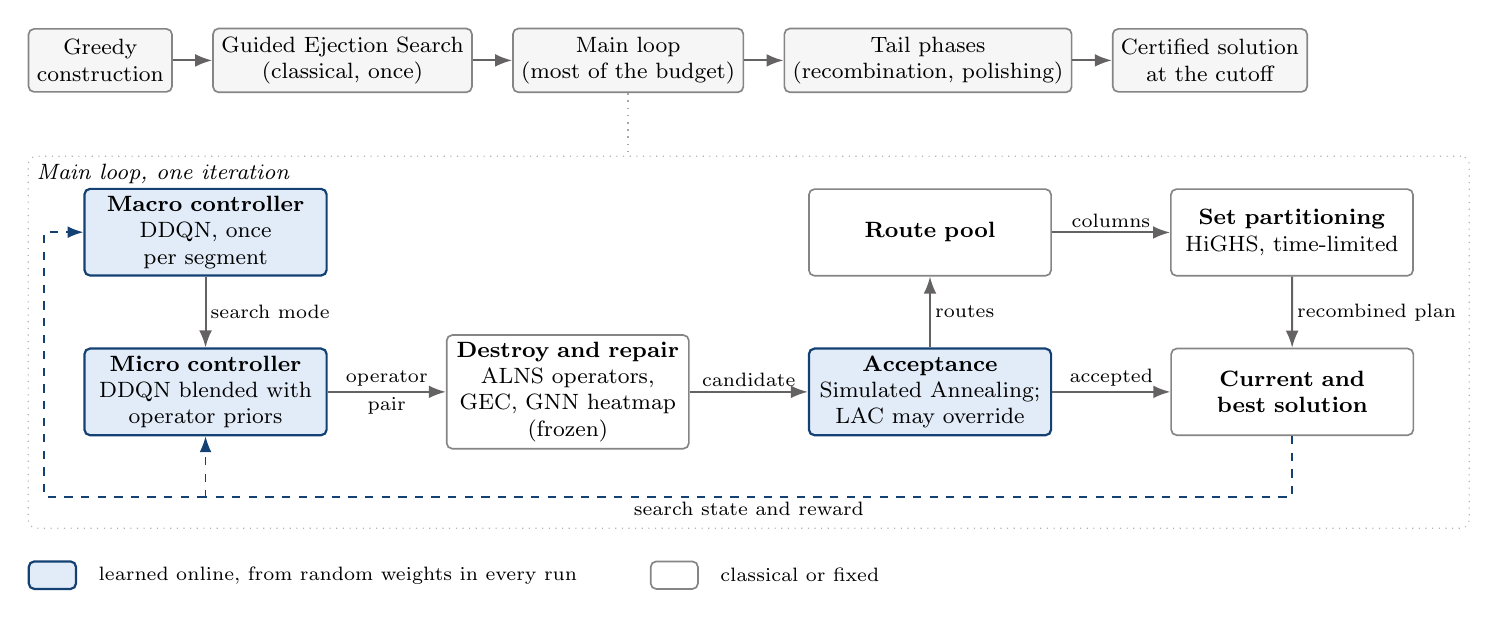
\begin{tikzpicture}[
  >=Latex, font=\footnotesize,
  box/.style={draw=black!55, fill=white, rounded corners=2pt, line width=0.6pt,
              text width=2.9cm, minimum height=11mm, align=center, inner sep=2.5pt},
  learned/.style={box, draw=cMacro, fill=cMacroBg, line width=0.8pt},
  phase/.style={draw=black!55, fill=black!4, rounded corners=2pt, line width=0.6pt,
                minimum height=8mm, align=center, inner sep=3pt},
  flow/.style={->, line width=0.7pt, draw=black!70},
  fb/.style={->, line width=0.6pt, draw=cMacro, dashed},
  lab/.style={font=\scriptsize, inner sep=1.5pt}
]
  % --- one iteration of the main loop ------------------------------------
  \node[learned] (macro) {\textbf{Macro controller}\\ DDQN, once per segment};
  \node[learned, below=9mm of macro] (micro) {\textbf{Micro controller}\\ DDQN blended with\\ operator priors};
  \node[box, right=15mm of micro] (alns) {\textbf{Destroy and repair}\\ ALNS operators,\\ GEC, GNN heatmap\\ (frozen)};
  \node[learned, right=15mm of alns] (lac) {\textbf{Acceptance}\\ Simulated Annealing;\\ LAC may override};
  \node[box, above=9mm of lac] (pool) {\textbf{Route pool}};
  \node[box, right=15mm of pool] (sp) {\textbf{Set partitioning}\\ HiGHS, time-limited};
  \node[box, right=15mm of lac] (inc) {\textbf{Current and}\\ \textbf{best solution}};

  \draw[flow] (macro) -- node[lab, right] {search mode} (micro);
  \draw[flow] (micro) -- node[lab, above] {operator} node[lab, below] {pair} (alns);
  \draw[flow] (alns) -- node[lab, above] {candidate} (lac);
  \draw[flow] (lac) -- node[lab, above] {accepted} (inc);
  \draw[flow] (lac) -- node[lab, right] {routes} (pool);
  \draw[flow] (pool) -- node[lab, above] {columns} (sp);
  \draw[flow] (sp) -- node[lab, right] {recombined plan} (inc);

  \coordinate (fbY) at ($(alns.south)+(0,-6mm)$);
  \draw[fb] (inc.south) |- node[lab, pos=0.75, below] {search state and reward} (fbY -| micro.south) -- (micro.south);
  \draw[fb] (fbY -| micro.south) -- ($(fbY -| macro.west)+(-5mm,0)$) |- (macro.west);

  \node[draw=black!35, dotted, rounded corners=3pt, inner xsep=7mm, inner ysep=4mm,
        fit=(macro) (micro) (alns) (lac) (pool) (sp) (inc) (fbY)] (loop) {};
  \node[font=\footnotesize\itshape, anchor=north west, inner sep=3pt] at (loop.north west) {Main loop, one iteration};

  % --- the whole run along the wall-clock budget ---------------------------
  \node[phase, above=8mm of loop.north west, anchor=south west] (start) {Greedy\\ construction};
  \node[phase, right=5mm of start] (ges) {Guided Ejection Search\\ (classical, once)};
  \node[phase, right=5mm of ges] (main) {Main loop\\ (most of the budget)};
  \node[phase, right=5mm of main] (tail) {Tail phases\\ (recombination, polishing)};
  \node[phase, right=5mm of tail] (out) {Certified solution\\ at the cutoff};
  \draw[flow] (start) -- (ges); \draw[flow] (ges) -- (main); \draw[flow] (main) -- (tail); \draw[flow] (tail) -- (out);
  \draw[black!40, line width=0.6pt, dotted] (main.south) -- (main.south |- loop.north);

  % --- legend ---------------------------------------------------------------
  \node[learned, text width=, minimum height=3.5mm, minimum width=6mm, below=4mm of loop.south west, anchor=north west] (k1) {};
  \node[right=1.5mm of k1, font=\scriptsize] (k1t) {learned online, from random weights in every run};
  \node[box, text width=, minimum height=3.5mm, minimum width=6mm, right=8mm of k1t] (k2) {};
  \node[right=1.5mm of k2, font=\scriptsize] {classical or fixed};
\end{tikzpicture}%
}
\DIFaddendFL \caption{Tri-Level Hybrid DDQN-ALNS .  \DIFaddbeginFL \DIFaddFL{Top: the phases of one run within the wall-clock budget}\DIFaddendFL .  \DIFaddbeginFL \DIFaddFL{Bottom: one iteration of }\DIFaddendFL the  \DIFaddbeginFL \DIFaddFL{main loop. Shaded components learn online from random weights in every run; the others are classical or fixed, }\DIFaddendFL and  \DIFaddbeginFL \DIFaddFL{the GNN heatmap comes from a frozen pretrained model}\DIFaddendFL . The  \DIFaddbeginFL \DIFaddFL{macro controller chooses a search mode once per }\DIFaddendFL segment  \DIFaddbeginFL \DIFaddFL{of iterations, and one mode triggers set partitioning over }\DIFaddendFL the  \DIFaddbeginFL \DIFaddFL{route pool. Dashed arrows carry the search state }\DIFaddendFL and  \DIFaddbeginFL \DIFaddFL{reward to the controllers}\DIFaddendFL .}
\label{fig:architecture}
\end{figure*}

\subsection{Macro Level: Plateau Controller (Aggregated SMDP Formulation)}
\label{sec:macro_controller}

We formulate the macro  tier as a Semi-Markov Decision Process\DIFaddbegin \DIFadd{~}\DIFaddend \cite{sutton1999between} over an Aggregated State Representation (Aggregated SMDP) defined by the tuple $(\mathcal{S}_{\text{macro}}, \mathcal{A}_{\text{macro}}, P_{\text{macro}}, R_{\text{macro}}, \gamma_{\text{macro}})$. Because the underlying combinatorial route pool and fine-grained trajectory history are projected into a  \DIFaddbegin \DIFadd{12-dimensional }\DIFaddend feature space $\mathbf{s}_k^{\text{macro}}$, the decision tier operates over a compact aggregated state representation with temporal options of fixed duration $\Delta_{\text{seg}} = 100$ low-level ALNS iterations. The \DIFaddbegin \DIFadd{controller acts only once the search has stagnated for a minimum number of iterations; before that, segments run in the default mode and are not used as macro transitions. The }\DIFaddend temporally extended transition kernel $P_{\text{macro}}(\mathbf{s}_{k+1}^{\text{macro}} \mid \mathbf{s}_k^{\text{macro}}, a_k)$  \DIFaddbegin \DIFadd{denotes the distribution of the next observation after the }\DIFaddend 100 underlying stochastic destroy--repair steps \DIFaddbegin \DIFadd{. The learner discounts per macro decision with $\gamma_{\text{macro}} = 0.95$, used both in the DDQN target and in the shaping term below, rather than with $\gamma^{\Delta_{\text{seg}}}$}\DIFaddend .

\DIFaddbegin \DIFadd{The aggregated formulation is a modeling device, not a verified Markov model. The 12 features are a lossy summary of the full search state, which also includes the current routes, the route pool, the operator weights, the network parameters and the random-number state. Distinct search states therefore share an observation, and the next observation depends on components that the controller does not see, so $\mathbf{s}_k^{\text{macro}}$ is not in general a sufficient statistic and the macro process need not satisfy the Markov property. The controller is better described as a learned policy over a partially observed, state-aggregated process~\mbox{%DIFAUXCMD
\cite{li2006unified}}\hskip0pt%DIFAUXCMD
. We provide no convergence guarantee and no bound on the approximation error. Such guarantees are not available in general for Q-learning over aggregated or partial observations, and the online DDQN additionally uses nonlinear function approximation, experience replay and target networks. The value of the controller is therefore assessed empirically through the ablation study (Section~\ref{sec:ablation_results}).
}

\DIFaddend \subsubsection{Macro State Representation}
At the start of segment $k$, the macro controller observes a  \DIFaddbegin \DIFadd{12-dimensional state vector }{\color{blue}$\mathbf{s}_k^{\text{macro}} \in \mathbb{R}^{12}$}\DIFadd{, covering search progress, fleet size and route structure}\DIFaddend :

 \DIFaddbegin \begin{align}
  \DIFadd{\mathbf{s}_k^{\text{macro}} = \Big[ 
    }&\DIFadd{\min\Big(\frac{\text{no\_imp}}{\text{patience}}, 1\Big), \; \min\Big(\frac{C_{\text{cur}} - C_{\text{best}}}{C_{\text{best}}}, 1\Big), \nonumber }\\
    &\DIFadd{\min\Big(\frac{T}{T_0}, 1.5\Big), \; \text{imp\_rate}, \; \min\Big(\frac{\NVs{cur}}{\NVs{init}}, 2\Big), \nonumber }\\
    &\DIFadd{\mathrm{rb}, \; \mathrm{lb}, \; \tau_{\text{tight}}, \nonumber }\\
    &\DIFadd{\bar{s}, \; \rho_{\text{fill}}, \; \rho_{\text{pool}}, \; \frac{k}{K_{\max}} \Big]
  \label{eq:macro_state}
}\end{align}\DIFaddend 

where $\text{no\_imp}$ is the number of consecutive unimproved iterations, $T/T_0$ is the normalized annealing temperature,  \DIFaddbegin \DIFadd{$\mathrm{rb} \in [0, 1]$ and $\mathrm{lb} \in [0, 1]$ }\DIFaddend measure spatial route separation and capacity balance,  \DIFaddbegin {\color{blue}$\tau_{\text{tight}} = \frac{1}{n}\sum_{i=1}^n \mathbb{I}(l_i - e_i < 0.5 \cdot d_{\max})$}\DIFadd{ is }\DIFaddend the fraction of  \DIFaddbegin \DIFadd{customers whose time-window width is below half the largest distance $d_{\max}$ of the instance}\DIFaddend , $\bar{s}$ is \DIFaddbegin \DIFadd{the }\DIFaddend average forward time slack, $\rho_{\text{fill}}$ is \DIFaddbegin \DIFadd{the }\DIFaddend average vehicle capacity utilization, and $\rho_{\text{pool}} = \min(|\mathcal{P}|/\mathcal{P}_{\max}, 1.0)$ tracks \DIFaddbegin \DIFadd{the }\DIFaddend route pool fill ratio.

\subsubsection{Macro Action Space \& Search Regimes}
The macro action space $\mathcal{A}_{\text{macro}}$ comprises 7  \DIFaddbegin \DIFadd{search modes. Each mode scales the destroy size, multiplies the temperature once per segment, biases the operator priors and sets the local-search passes. With (destroy scale, temperature factor) in parentheses, the modes are}\DIFaddend : $a_0$ (\textsf{\small DEFAULT} \DIFaddbegin \DIFadd{, 1.00, 1.00)}\DIFaddend ; $a_1$ (\textsf{\small  \DIFaddbegin \DIFadd{INTENSIFY}}\DIFadd{, 0.70, 0.98)}\DIFaddend ; $a_2$ (\textsf{\small DIVERSIFY} \DIFaddbegin \DIFadd{, 1.35, 1.08), which also permits a one-vehicle increase in the current solution}\DIFaddend ; $a_3$ (\textsf{\small TW\_RESCUE} \DIFaddbegin \DIFadd{, 1.10, 1.05), with priors favoring time-window urgency removal and time-window-aware repair}\DIFaddend ; $a_4$ ( \textsf{\small POOL\_RECOMBINE} \DIFaddbegin \DIFadd{, 0.90, 1.01), which may trigger Set Partitioning}\DIFaddend ; \DIFaddbegin \DIFadd{$a_5$ (}\textsf{\small \DIFadd{ROUTE\_REDUCE}}\DIFadd{, 0.95, 1.02), with priors favoring route-elimination operators, a Generalized Ejection Chain attempt at every iteration, penalized acceptance, and possible recombination; }\DIFaddend and $a_6$ (\textsf{\small INFEASIBLE\_DESCENT} \DIFaddbegin \DIFadd{, 1.10, 1.05), which is available only during the first search phase described below and maps to }\textsf{\small \DIFadd{DEFAULT}} \DIFadd{afterwards. The segment length is 100 iterations, or 130 on instances with wide time windows}\DIFaddend .

\DIFaddbegin \subsubsection{Search Phases}
\label{sec:search_phases}
\DIFadd{The search changes behavior over the budget. In the first phase, candidates are accepted by a penalized Simulated Annealing rule on }{\color{blue}$C_{\text{pen}}(s) = C(s) + \lambda\,(v_{\text{cap}}(s) + v_{\text{tw}}(s))$}\DIFadd{, so the current solution may be infeasible. The multiplier $\lambda$ is updated every 100 iterations, by a factor of 0.90 when more than half of recent candidates are feasible and 1.15 otherwise, and is bounded by $[5, 200]$ for instances with tight time windows and $[0.5, 50]$ for others. The phase ends after 60\% of a nominal 10,000 iterations, when the fleet reaches its floor, or, with no known floor, after 250 iterations without a new best solution (and at least 200 iterations in total). LAC is not consulted in this phase, and mode $a_5$ also keeps penalized acceptance afterwards.
}

\DIFadd{The main destroy-repair loop receives $80\%$ of the time budget. The remaining $20\%$ goes to tail phases: pool recombination, polishing at fixed fleet size, dense column generation for the pool, route-elimination heuristics, and distance polishing. ALNS-Base has no tail phases. A few settings also adapt to the instance: the initial temperature is scaled by 0.8 for tight and 1.2 for wide time windows, and the plateau trigger is 1.5 times longer for $N \ge 200$.
}

\DIFaddend \subsubsection{Multi-Objective Segment Reward \& Surrogate Policy Optimization}
 \DIFaddbegin \DIFadd{The }\DIFaddend segment reward $R_{\text{seg}}$  \DIFaddbegin \DIFadd{weighs vehicle reduction }\DIFaddend against distance savings  \DIFaddbegin \DIFadd{through }\DIFaddend an adaptive fleet pressure factor $\lambda_{\text{fleet}} \in [0, 1]$:
 \DIFaddbegin \begin{equation}
  \begin{split}
    \DIFadd{R_{\text{seg}} = 0.30\big[}&\DIFadd{\text{Base} + \lambda_{\text{fleet}} \Psi_{\mathrm{NV}} + (1 - \lambda_{\text{fleet}}) \Psi_{\mathrm{TD}} }\\
    &\DIFadd{+ \text{Bonus}_{\mathrm{NV}}\big] + \Delta \Phi
  }\end{split}
  \DIFadd{\label{eq:segment_reward}
}\end{equation}\DIFaddend 
where  \DIFaddbegin {\color{blue}$\Psi_{\mathrm{NV}} = \sum_{j=1}^4 \beta_{\mathrm{NV}, j} \Delta X_j$} \DIFaddend and \allowbreak  \DIFaddbegin {\color{blue}$\Psi_{\mathrm{TD}} = \sum_{j=1}^4 \beta_{\mathrm{TD}, j} \Delta X_j$} \DIFaddend linearly weight improvements across best-so-far and incumbent fleet size ( \DIFaddbegin \DIFadd{$\Delta\NV$}\DIFaddend ) and travel distance ($\Delta C$), with \DIFaddbegin \DIFadd{a }\DIFaddend representative primary fleet coefficient  \DIFaddbegin \DIFadd{$\beta_{\mathrm{NV}, 1} = 8.0$. The baseline term }\DIFaddend $\text{Base}$ penalizes intensive local search passes and unproductive stagnation, while  \DIFaddbegin \DIFadd{$\text{Bonus}_{\mathrm{NV}}$ provides a discrete reward of $+15$ per vehicle removed from the best solution and $+5$ per vehicle removed from the current solution. All coefficients are listed in Supplementary Section~6.
}\DIFaddend 

 \DIFaddbegin \DIFadd{Equation~\eqref{eq:segment_reward} has two fleet rewards. The dense term ($\lambda_{\text{fleet}} \Psi_{\mathrm{NV}}$) rewards }\DIFaddend moves that balance  \DIFaddbegin \DIFadd{route loads }\DIFaddend and narrow the  \DIFaddbegin \DIFadd{fleet gap }\DIFaddend to the incumbent \DIFaddbegin \DIFadd{. The sparse term ($\text{Bonus}_{\mathrm{NV}}$) pays only when a vehicle is removed, so that signal is not diluted by routine changes in distance}\DIFaddend .

\paragraph{ Reward  \DIFaddbegin \DIFadd{Constants}\DIFaddend }
 \DIFaddbegin \DIFadd{The reward constants were set by hand during development, and Section~\ref{sec:setup} states what we can and cannot document about them and how the test set influenced later development.
}\DIFaddend 

 \DIFaddbegin \DIFadd{Evaluation and training use different objectives. }\DIFaddend Incumbent replacement, elite archive admission  \DIFaddbegin \DIFadd{and final selection use the lexicographic order $f(s) = (\NV(s), \TD(s))$, so fleet size always comes before distance. The policy instead receives the scalar reward }\DIFaddend $R_{\text{seg}}$\DIFaddbegin \DIFadd{, }\DIFaddend modulated by $\lambda_{\text{fleet}}$. When  \DIFaddbegin \DIFadd{the current fleet is above the best ($\NVs{cur} > \NVs{best}$), }\DIFaddend $\lambda_{\text{fleet}} \to 1$ concentrates  \DIFaddbegin \DIFadd{the reward on removing vehicles; once they match ($\NVs{cur} = \NVs{best}$), }\DIFaddend $\lambda_{\text{fleet}} \le 0.5$  \DIFaddbegin \DIFadd{moves the weight to }\DIFaddend distance.

 \DIFaddbegin \DIFadd{We also add potential-based reward shaping }{\color{blue}$\Delta \Phi = \gamma_{\text{macro}}\,\Phi(\mathbf{s}_{k+1}^{\text{macro}}) - \Phi(\mathbf{s}_k^{\text{macro}})$}\DIFadd{ to speed up learning without creating }\DIFaddend artificial reward cycles in the surrogate MDP \DIFaddbegin \DIFadd{. This shaping applies to }\DIFaddend the \emph{macro surrogate objective} \cite{ng1999policy} \DIFaddbegin \DIFadd{. It does not give }\DIFaddend policy invariance with respect to the  lexicographic VRPTW objective \DIFaddbegin \DIFadd{, which the evaluator enforces separately. The }\DIFaddend fleet pressure factor  \DIFaddbegin \DIFadd{rises when the current fleet is above the best:
}\begin{equation}
  \DIFadd{\lambda_{\text{fleet}}(s) = \sigma\!\left(8.0 \cdot \frac{\NVs{cur} - \NVs{best}}{\NVs{init}}\right)
  \label{eq:lambda_fleet}
}\end{equation}\DIFaddend 
where $\sigma(\cdot)$ is the logistic sigmoid, with the state potential defined as:
 \DIFaddbegin \begin{align}
  \DIFadd{\Phi(s) = }&\DIFadd{-15\,\lambda_{\text{fleet}}(s) \frac{\max(\NV - \NVs{best}, 0)}{\NVs{init}} \nonumber }\\
  &\DIFadd{- 0.18\bigl(1 - \lambda_{\text{fleet}}(s)\bigr) \nonumber }\\
  &\DIFadd{\quad \times \operatorname{clip}\!\left(\frac{\TD - \TDs{best}}{\TDs{best}} \cdot 100, -25, 25\right)
  \label{eq:potential_function}
}\end{align}\DIFaddend 
The Macro Plateau Controller trains  \DIFaddbegin \DIFadd{its own }\DIFaddend Dueling Double DQN  ($Q_{\text{macro}}$) with prioritized replay buffer $\mathcal{D}_{\text{macro}}$,  \DIFaddbegin \DIFadd{taking Adam steps with a cosine-annealed learning rate at the end }\DIFaddend of each macro segment.

\subsection{Micro Level: Operator Controller \& Action Blending}
\label{sec:micro_controller}

\subsubsection{Micro State Representation}
At each iteration $t$, the operator controller observes a 20-dimensional state vector $\mathbf{s}_t^{\text{micro}} \in \mathbb{R}^{20}$ (Table~\ref{tab:micro_state}),  \DIFaddbegin \DIFadd{which describes search progress and route structure}\DIFaddend .

\begin{table}[!b]
\caption{20-Dimensional Micro State Vector $\mathbf{s}_t^{\text{micro}}$}
\label{tab:micro_state}
\centering
\scriptsize
\setlength{\tabcolsep}{1.2pt}
\begin{tabularx}{\columnwidth}{cl>{\raggedright\arraybackslash}X cl>{\raggedright\arraybackslash}X}
\toprule
\textbf{Idx} & \textbf{Sym} & \textbf{Definition} & \textbf{Idx} & \textbf{Sym} & \textbf{Definition} \\
\midrule
$s_1$ & $\Delta C_{\text{rel}}$ & $(C_{\text{cur}}\!-\!C_{\text{best}})/C_{\text{best}}$ & $s_{11}$ & $\rho_{\text{fill}}$ & Capacity fill ratio \\
$s_2$ &  \DIFaddbeginFL \DIFaddFL{$\text{Ratio}_{\mathrm{NV}}$ }\DIFaddendFL &  \DIFaddbeginFL \DIFaddFL{$\NVs{cur}/\NVs{init}$ }\DIFaddendFL & $s_{12}$ & $\rho_{\text{pool}}$ & Pool fill ratio $|\mathcal{P}|/\mathcal{P}_{\max}$ \\
$s_3$ & $\text{Prog}_{\text{global}}$ &  \DIFaddbeginFL \DIFaddFL{$\min(t / 10000, 1)$ }\DIFaddendFL & $s_{13}$ & $m_{\text{idx}}$ & Active macro mode index \\
$s_4$ & $\text{Prog}_{\text{seg}}$ & $(t \bmod \Delta_{\text{seg}})/\Delta_{\text{seg}}$ & $s_{14}$ &  \DIFaddbeginFL \DIFaddFL{$\Delta \NVs{rel}$ }\DIFaddendFL &  \DIFaddbeginFL \DIFaddFL{$(\NVs{cur}\!-\!\NVs{best})/\NVs{init}$ }\DIFaddendFL \\
$s_5$ & $T_{\text{norm}}$ & $T / T_0$ & $s_{15}$ & $\text{Imp}_{\text{rec}}$ & Recent improvement rate \\
$s_6$ & $\text{Stag}_{\text{ratio}}$ & $\text{no\_imp} / \text{patience}$ & $s_{16}$ & $\text{Gini}_{\text{len}}$ & Gini of route  \DIFaddbeginFL \DIFaddFL{loads }\DIFaddendFL \\
$s_7$ &  \DIFaddbeginFL \DIFaddFL{$\mathrm{rb}$ }\DIFaddendFL & Route separation index & $s_{17}$ & $\mu_{\text{slack}}$ & Mean customer forward slack \\
$s_8$ &  \DIFaddbeginFL \DIFaddFL{$\mathrm{lb}$ }\DIFaddendFL & Capacity load balance & $s_{18}$ & $\sigma_{\text{slack}}$ & Std of forward slacks \\
$s_9$ & $\tau_{\text{tight}}$ & Frac tight TW customers & $s_{19}$ & $\text{Frac}_{\text{cap}}$ & Fraction routes $>90\%$ cap \\
$s_{10}$ & $\bar{s}$ & Normalized mean slack & $s_{20}$ & $\text{Var}_{\text{dist}}$ &  \DIFaddbeginFL \DIFaddFL{Normalized variance of route distances }\DIFaddendFL \\
\bottomrule
\end{tabularx}
\end{table}

\subsubsection{Composite Action Space}
The micro action space $\mathcal{A}_{\text{micro}}$ comprises $N_D \times N_R = 13 \times 5 = 65$ composite heuristic pairs, combining 13 Destroy Operators (Random, Worst-cost, Shaw spatiotemporal relatedness, Route portion removal, Time-window urgency removal, Route-Depletion Destroy, Route dispersion elimination, Costly route elimination, Cross-route Shaw, Route merge sampling, Route absorb disruption, Neural worst, Neural Shaw) with 5 Repair Operators (Greedy insertion, 2-Regret, 3-Regret, Time-window greedy, Forward-time-slack greedy).

\subsubsection{Dueling DDQN Architecture \& Policy-Concentration Blending}
The Micro Q-network adopts a Dueling architecture \cite{wang2016dueling} with layer normalization:
\begin{equation}
  Q(s, a; \theta) = V(s; \theta_v) + \Big( A(s, a; \theta_a) - \frac{1}{|\mathcal{A}|} \sum_{a'} A(s, a'; \theta_a) \Big)
  \label{eq:dueling_q}
\end{equation}
 \DIFaddbegin \DIFadd{A }\DIFaddend normalized Softmax-Entropy Policy-Concentration Gate \DIFaddbegin \DIFadd{balances the Q-values against the exploration priors}\DIFaddend . Let $\pi_{\theta}(a \mid s) = \operatorname{softmax}(Q(s, a)/\tau_{\text{soft}})$ be the Boltzmann policy at softmax temperature $\tau_{\text{soft}} = 1.0$. The normalized Shannon entropy is defined as:
\begin{equation}
  \mathcal{H}(\pi_{\theta}(\cdot \mid s)) = -\frac{1}{\ln |\mathcal{A}|} \sum_{a \in \mathcal{A}} \pi_{\theta}(a \mid s) \ln \pi_{\theta}(a \mid s) \in [0, 1]
  \label{eq:policy_entropy}
\end{equation}
We define the policy-concentration weight as $w_{\text{conf}}(s) = 1.0 - \mathcal{H}(\pi_{\theta}(\cdot \mid s))$. High concentration ($w_{\text{conf}} \to 1$) indicates that the Boltzmann policy is sharply peaked around a dominant operator pair, whereas low concentration ($w_{\text{conf}} \to 0$) signals an exploratory regime.

 \DIFaddbegin \DIFadd{The }\DIFaddend action-selection score  \DIFaddbegin \DIFadd{blends the }\DIFaddend Q-values with  \DIFaddbegin \DIFadd{operator }\DIFaddend priors and the \DIFaddbegin \DIFadd{mean of a Thompson-sampling posterior through this gate, then adds a }\DIFaddend variance-aware  bonus adapted from UCB \cite{auer2002finite} and UCB-V \cite{audibert2009exploration} \DIFaddbegin \DIFadd{:
}\begin{align}
  \DIFadd{Q_{\text{blend}}(s, a) = \; }&\DIFadd{w_{\text{conf}}(s)\,Q(s, a) + (1 - w_{\text{conf}}(s))\big[ \alpha_{\text{p}}\ln P(a) \nonumber }\\
  &\DIFadd{+ \beta_{\text{b}}\,\bar{\mu}_{\text{bandit}}(a) \big], \nonumber }\\
  \DIFadd{Q_{\text{eff}}(s, a) = \; }&\DIFadd{Q_{\text{blend}}(s, a) + \alpha_{\text{u}}\,\frac{U(a) - \bar{U}}{\sigma_U}, \nonumber }\\
  \DIFadd{U(a) = \; }&\DIFadd{\hat{\mu}(a) + c_{\text{ucb}}\,\sigma_a \sqrt{\ln N_t / N_a(t)},
  \label{eq:q_eff_blending}
}\end{align}\DIFaddend 
where  \DIFaddbegin \DIFadd{$\alpha_{\text{p}} = 0.55$ }\DIFaddend scales prior log-probabilities,  \DIFaddbegin \DIFadd{$\beta_{\text{b}} = 0.20$ weights the bandit posterior mean, $\alpha_{\text{u}} = 0.35$ weights the standardized bonus over the actions, }\DIFaddend $c_{\text{ucb}} = 1.0$ , \DIFaddbegin \DIFadd{$\hat{\mu}(a)$ is a running mean reward, }\DIFaddend and $\sigma_a = \sqrt{M_{2, a}/\max(N_a(t) - 1, 1)}$  \DIFaddbegin \DIFadd{is an online }\DIFaddend standard deviation tracked  \DIFaddbegin \DIFadd{with }\DIFaddend Welford's algorithm. Action counters  \DIFaddbegin \DIFadd{start at $0.5$ and decay by $0.993$ per step, and }\DIFaddend $N_t = \sum_a N_a(t)$ .

 \DIFaddbegin \DIFadd{Two properties of this rule follow directly. The Q-values and log-priors are not standardized before the gate, so the balance between them depends on the scale of the learned values. The bonus is not gated, so it continues to affect selection when the policy is concentrated}\DIFaddend .

\DIFaddbegin \DIFadd{The first 256 transitions select pairs from the bandit with the prior. After that, the controller explores with probability $\varepsilon$, sampling from the prior and bandit, with $\varepsilon$ decaying from $0.35$ to $0.02$ by a factor of $0.9996$ per step. It otherwise takes the pair that maximizes $Q_{\text{eff}}$. The Micro reward has the same form as $R_{\text{seg}}$ at iteration level, with its own coefficients and a scale of $0.45$; a rejected candidate receives a base reward of $-0.08$ before shaping.
}

\DIFaddend \subsection{Learned Acceptance Criterion (LAC): SA with Predictive Lookahead Override}
\label{sec:lac}

In classical ALNS, move acceptance relies on Simulated Annealing (SA), which accepts improving transitions ($\Delta C < 0$) deterministically and non-improving transitions ($\Delta C \ge 0$) with probability $P_{\text{SA}} = \exp(-\Delta C / T)$. During deep cooling stages ($T \to 0$), $P_{\text{SA}}$ vanishes exponentially, restricting search to downhill moves \DIFaddbegin \DIFadd{, so the search can get stuck in local optima}\DIFaddend .

To  \DIFaddbegin \DIFadd{reduce this trapping}\DIFaddend , the Learned Acceptance Criterion (LAC)  \DIFaddbegin \DIFadd{adds }\DIFaddend an online supervised binary classifier $\phi_{\text{LAC}}: \mathbb{R}^9 \to [0, 1]$.  \DIFaddbegin \DIFadd{LAC is consulted only for feasible candidates that keep the current fleet size and increase travel distance; improving, fleet-reducing and infeasible candidates follow the rules of Algorithm~\ref{alg:hybrid_ddqn_alns} unchanged, and penalty-relaxed phases use the penalized SA rule without LAC. For these candidates, LAC does not filter or replace SA. It adds a disjunctive }\DIFaddend rule:
\begin{equation}
\begin{aligned}
  \text{Accept}(s' \mid s, T) \iff \; &\Big( p_t \ge \tau_{\text{acc}}(t) \Big) \\
  &\lor\; \Big( P_{\text{SA}}(\Delta C, T) > U \Big)
\end{aligned}
\label{eq:lac_decision_rule}
\end{equation}
where $p_t = \phi_{\text{LAC}}(\mathbf{z}_t)$, $U \sim \operatorname{Uniform}(0, 1)$, and $\tau_{\text{acc}}(t) \in [0.40, 0.75]$ is an adaptive confidence threshold.

 \DIFaddbegin \DIFadd{The disjunction }\DIFaddend ($\lor$)  \DIFaddbegin \DIFadd{means LAC can only add acceptances. Any consulted move that }\DIFaddend standard Simulated Annealing \DIFaddbegin \DIFadd{would accept }\DIFaddend ($P_{\text{SA}} > U$) is  \DIFaddbegin \DIFadd{also accepted by rule~\eqref{eq:lac_decision_rule}. When SA would reject }\DIFaddend a non-improving move ($P_{\text{SA}} \le U$) \DIFaddbegin \DIFadd{, }\DIFaddend the  \DIFaddbegin \DIFadd{move is still accepted if the classifier predicts a later incumbent improvement with probability $p_t \ge \tau_{\text{acc}}(t)$. These extra transitions mean that rule~\eqref{eq:lac_decision_rule} defines a different Markov transition kernel from SA, and the classical asymptotic convergence results for SA under logarithmic cooling~\mbox{%DIFAUXCMD
\cite{hajek1988cooling} }\hskip0pt%DIFAUXCMD
do not carry over. We make no convergence claim for the modified kernel: the search uses geometric cooling within a finite budget, and the contribution of LAC is assessed empirically (Section~\ref{sec:ablation_results}). The supervision target is observational. The first $W_{\text{lac}} = 300$ consulted decisions use pure SA while the classifier collects training data; for every consulted move, including warmup moves, the label records whether the global best travel distance improved within the next $H_{\text{lac}} = 80$ LAC decisions (not 80 ALNS iterations), irrespective of whether the move was accepted. The label therefore indicates a promising search context rather than the causal effect of accepting that particular move.
}\DIFaddend 

Because  rule~\eqref{eq:lac_decision_rule}  \DIFaddbegin \DIFadd{only adds acceptances, it increases the number }\DIFaddend of accepted non-improving  \DIFaddbegin \DIFadd{moves }\DIFaddend during deep cooling.  Sections~\ref{sec:ablation_results} and~\ref{sec:disc_limitations}  \DIFaddbegin \DIFadd{return to the difficulty of separating useful lookahead from a higher acceptance rate}\DIFaddend .

 \DIFaddbegin \subsubsection{Features and Training}
\DIFaddend The LAC input feature vector $\mathbf{z}_t \in \mathbb{R}^9$ comprises 9 normalized features:
 \DIFaddbegin \begin{align}
  \DIFadd{\mathbf{z}_t = \Big[
    }&\DIFadd{\frac{\Delta C}{|C_{\text{cur}}|}, \; \frac{T}{T_0}, \; \frac{\text{no\_imp}}{\text{patience}}, \nonumber }\\
    &\DIFadd{\operatorname{clip}(\Delta\NV, -2, 2), \; \min\Big(\frac{t}{10000}, 1\Big), \nonumber }\\
    &\DIFadd{\tau_{\text{tight}}, \; \rho_{\text{fill}}, \; \bar{s}, \; \exp\left(-\frac{\max(\Delta C, 0)}{T}\right) \Big]
  \label{eq:lac_features}
}\end{align}\DIFaddend 
During the first 300  \DIFaddbegin \DIFadd{consulted decisions}\DIFaddend , the solver  \DIFaddbegin \DIFadd{uses Simulated Annealing alone while queuing the features of each decision. After a further $H_{\text{lac}} = 80$ consulted decisions, each queued decision receives a binary label: $y_t = 1$ if the best distance $C_{\text{best}}$ has decreased since that decision, and $0$ otherwise. The label therefore follows distance, not the lexicographic objective, so a fleet reduction that raises the best distance receives $y_t = 0$. The threshold rises with progress $p = \min(t/10000, 1)$ as $\tau_{\text{acc}}(t) = 0.40 + 0.35\,p^{0.75}$.
}\DIFaddend 

Because training examples are labeled online from the active search trajectory, the empirical training distribution is endogenous and non-stationary. \DIFaddbegin \DIFadd{Every 20 consulted decisions, }\DIFaddend LAC trains a  4-layer MLP ($9 \to 64 \to 48 \to 32 \to 1$ \DIFaddbegin \DIFadd{, with LayerNorm and $0.1$ dropout after the first layer) on a batch of 64 from a buffer of 5,000 labeled decisions, using Adam }\DIFaddend ($\text{lr} = 10^{-3}$) with class-weighted binary cross-entropy loss:
\begin{equation}
  \mathcal{L}_{\text{LAC}}(\phi) = -\frac{1}{B} \sum_{i=1}^B \Big[ w_1 y_i \log p_i + (1 - y_i) \log (1 - p_i) \Big]
  \label{eq:lac_loss}
\end{equation}
where $p_i = \phi_{\text{LAC}}(\mathbf{z}_i)$ and $w_1 = N_{\text{neg}} / N_{\text{pos}}$ balances positive  \DIFaddbegin \DIFadd{and negative labels within the batch}\DIFaddend .

 \DIFaddbegin \subsection{Heuristic Search Components}
\DIFaddend \label{sec:search_muscle}

 \DIFaddbegin \DIFadd{The }\DIFaddend low-level  \DIFaddbegin \DIFadd{search combines cached insertion checks, granular candidate lists, a frozen GNN heatmap and ejection chains}\DIFaddend .

 \DIFaddbegin \subsubsection{Constant-Time Insertion Feasibility Queries via Savelsbergh Forward Slack}
\DIFadd{To avoid an }\DIFaddend $O(m)$  \DIFaddbegin \DIFadd{recomputation of route timing for each candidate insertion}\DIFaddend , we maintain Savelsbergh forward time slack $F_i$ for each node $i$ along route $R = (v_0, v_1, \dots, v_m)$ \cite{savelsbergh1992general}:
 \DIFaddbegin \begin{equation}
  \DIFadd{F_i = \min_{i \le j \le m} \left\{ l_j - w_j + \sum_{k=i+1}^{j} W_k \right\}
  \label{eq:forward_slack}
}\end{equation}\DIFaddend 
A candidate insertion of customer $u$ between positions $i$ and $i+1$ inducing arrival delay $\Delta t_u$ at node $i+1$ preserves temporal feasibility for all subsequent customers if and only if  \DIFaddbegin \DIFadd{$\max(0, \Delta t_u - W_{i+1}) \le F_{i+1}$, where $W_k$ is the waiting time at node $k$, given that the prefix up to $v_i$ is feasible and $u$ is served within its window; capacity feasibility additionally requires }\DIFaddend $q(R) + q_u \le Q$ \DIFaddbegin \DIFadd{. Given a cached timing profile of the route (arrival times, load, and forward slacks or, equivalently, the latest feasible service start of each node, which our implementation stores), each such query costs }\DIFaddend $O(1)$ . The arrival time delay shifted to customer $v_{i+1}$ is computed as:
\begin{equation}
  \Delta t_u = \max\bigl(0, e_u - (w_i + s_i + t_{i, u})\bigr) + t_{i, u} + s_u + t_{u, i+1} - t_{i, i+1}
  \label{eq:delta_t_insertion}
\end{equation}
where $w_i$ is  \DIFaddbegin \DIFadd{the service start }\DIFaddend time at node $i$, $s$ denotes service durations, and $e_u$ is \DIFaddbegin \DIFadd{the }\DIFaddend earliest ready time.  \DIFaddbegin \DIFadd{The $O(1)$ bound applies to a single insertion query and holds only while the cached profile is valid. Building or refreshing the profile costs $O(m)$ for a route }\DIFaddend of length $m$  \DIFaddbegin \DIFadd{and is required after every accepted modification of that route; scanning all $m+1$ insertion positions of one customer is therefore }\DIFaddend $O(m)$  \DIFaddbegin \DIFadd{per route, and evaluating one customer against $K$ routes is $O(Km)$ before granular pruning. Moves that reverse or relocate a segment (2-opt, ejection chains) recompute arrival times }\DIFaddend along the modified  \DIFaddbegin \DIFadd{segment, so their cost grows with the segment length, and only the suffix check after the segment uses the cached slack. We claim no $O(1)$ bound for complete moves or iterations.
}\DIFaddend 

\subsubsection{Granular Correlated Neighborhood Search (GNS)}
Following granular search principles \cite{toth2003granular}, inter-route operators restrict candidate evaluations to  \DIFaddbegin \DIFadd{the $k=15$ nearest customers of each customer by travel distance, precomputed once per instance with the depot excluded}\DIFaddend . This bounds the candidate insertion search space to $O(k N)$ move queries per iteration.

\subsubsection{Lightweight Graph Neural Network for Spatial Edge Guidance}
\label{sec:gnn_guidance}
 \DIFaddbegin \DIFadd{A }\DIFaddend lightweight Graph Neural Network (GNN)  \DIFaddbegin \DIFadd{adds a learned }\DIFaddend edge probability heatmap $\mathbf{H} \in [0, 1]^{(N+1)\times (N+1)}$ \DIFaddbegin \DIFadd{to the heuristic candidate lists}\DIFaddend . The graph encodes $N+1$ nodes (depot + customers) with 6-dimensional normalized node features $\mathbf{v}_i \in \mathbb{R}^6$:
\begin{equation}
  \mathbf{v}_i = \left[ \tilde{x}_i, \; \tilde{y}_i, \; \frac{q_i}{Q}, \; \frac{e_i}{T_{\text{depot}}}, \; \frac{l_i}{T_{\text{depot}}}, \; \frac{s_i}{T_{\text{depot}}} \right]
  \label{eq:gnn_node_feats}
\end{equation}
where $(\tilde{x}_i, \tilde{y}_i) \in [0, 1]^2$ are min-max normalized Cartesian coordinates, $q_i / Q$ is demand normalized by vehicle capacity, and $(e_i, l_i, s_i)$ are ready time, due time, and service duration normalized by the depot operational horizon $T_{\text{depot}}$. Message passing runs over sparse $k$-nearest-neighbor edge sets ($K=16$, with slot 0 pinned to the depot) with 1-dimensional edge feature $e_{ij} = c_{ij} / c_{\max}$ representing normalized Euclidean distance.

The network architecture comprises a linear embedding layer ($d_h = 64$), 3 sparse joint node-edge message-passing layers with LayerNorm and residual connections, and a bilinear projection head:
\begin{equation}
  \mathbf{H}_{ij} = \sigma\left( \mathbf{z}_i^{\top} \mathbf{W}_{\text{edge}} \mathbf{z}_j \right)
  \label{eq:gnn_bilinear_head}
\end{equation}
producing edge selection probabilities $\mathbf{H}_{ij} \in [0, 1]$.  \DIFaddbegin \DIFadd{Message passing uses the 16 nearest neighbors of each node. The registered checkpoint was trained offline with a weighted binary cross-entropy loss and sampled negative edges on 48 synthetic instances }\DIFaddend (\DIFaddbegin \DIFadd{16 each of the C, R and RC distributions, half with }\DIFaddend $N=100$  \DIFaddbegin \DIFadd{and half with $N=200$), with 12 further synthetic validation instances of the same sizes. Training targets are the route edges of a 10-second ALNS run without the GNN, so they are heuristic labels and not optimal edges. The checkpoint was selected by minimum validation loss (epoch 71 of 150, Adam, learning rate $10^{-3}$, one training seed), and no benchmark test instance was used for training or selection. On the 12 validation instances, thresholds of 0.05, 0.01 and 0.003 retain $23.3\%$, $29.6\%$ and $34.1\%$ of candidate arcs and $99.45\%$, $99.90\%$ and $99.90\%$ of teacher edges. These instances also selected the checkpoint, so the figures are optimistic, and they measure agreement with heuristic labels, not a routing gain. On the 74 benchmark instances at threshold 0.01, the heatmap retained $34.0\%$, $23.3\%$ and $23.6\%$ of candidate arcs at 100, 200 and 400 customers and kept $99.1\%$, $99.8\%$ and $100.0\%$ of the route edges in the PyVRP-ILS solutions of the rerun at 300\,s, and $98.0\%$, $99.2\%$ and $99.8\%$ of those of NeuroLKH-adapted. The lowest figure over the three thresholds was $96.6\%$, for NeuroLKH-adapted at 100 customers and threshold 0.05. These figures measure agreement with the routes of other solvers, which are themselves heuristic, and not a routing gain. The effect of the GNN on solutions is estimated only by the factorial ablation. }\DIFaddend $N=400$  \DIFaddbegin \DIFadd{lies outside the training sizes, so use at that size is an extrapolation}\DIFaddend . During search, network weights are frozen, and inference is executed once per instance during preprocessing in $O(N K)$ time, populating a static  \DIFaddbegin \DIFadd{heatmap }\DIFaddend $\mathbf{H}$ that  \DIFaddbegin \DIFadd{guides repair and filters insertion positions}\DIFaddend .

 \DIFaddbegin \subsubsection{Generalized Ejection Chains (GEC)}
\DIFaddend \label{sec:gec_methodology}
To  \DIFaddbegin \DIFadd{attack }\DIFaddend vehicle-count plateaus \DIFaddbegin \DIFadd{, a }\DIFaddend 3-level  \DIFaddbegin \DIFadd{ejection chain tries to eliminate the shortest route. It is attempted at every iteration in mode $a_5$, every fourth iteration when a route has at most four customers, and every twentieth consecutive iteration without improvement. Customers of the target route are processed by decreasing demand, and each displaced customer $u$ triggers a search over all other routes}\DIFaddend :
\begin{itemize}
    \item[(i)] Level 1 (Direct Insertion):  \DIFaddbegin \DIFadd{insert }\DIFaddend $u$ into  \DIFaddbegin \DIFadd{another }\DIFaddend route $R_j$  \DIFaddbegin \DIFadd{at minimum added distance}\DIFaddend ;
    \item[(ii)] Level 2 (Single-Customer Displacement): eject  $v \in R_j$, insert  \DIFaddbegin \DIFadd{$u$ into $R_j$}\DIFaddend , and insert  $v$ into a third route $R_k$; and
    \item[(iii)] Level 3 (Two-Customer Chained Displacement): eject $v \in R_j$  \DIFaddbegin \DIFadd{and }\DIFaddend insert $u$; eject $w \in R_k$  \DIFaddbegin \DIFadd{and }\DIFaddend insert $v$; and insert  \DIFaddbegin \DIFadd{$w$ into a further route. This level runs only when at most 30 routes remain.
}\end{itemize}
\DIFadd{The search has no candidate beam and no internal time check, so the solver can stop it only after it returns, while the supervisor enforces the cutoff independently. Each feasibility test replays the modified route at linear cost, not the $O(1)$ cached query above. For $m$ displaced customers, }\DIFaddend $K$ routes  \DIFaddbegin \DIFadd{and maximum route length $L$, the }\DIFaddend worst-case  \DIFaddbegin \DIFadd{work is $O(m K^3 L^4)$ (Supplementary Section}\DIFaddend ~3).

\subsubsection{Feasibility Invariant Across Operational Layers}
\label{sec:feasibility_invariant}
 \DIFaddbegin \DIFadd{Feasibility differs by operational level}\DIFaddend : (1)  \DIFaddbegin \DIFadd{Current solution }\DIFaddend ($s_{\text{cur}}$): may  \DIFaddbegin \DIFadd{be infeasible under penalized acceptance (Section~\ref{sec:search_phases}}\DIFaddend ); (2) Candidate  \DIFaddbegin \DIFadd{moves }\DIFaddend ($s_{\text{cand}}$):  \DIFaddbegin \DIFadd{violations are penalized in those phases and rejected otherwise}\DIFaddend ; (3)  \DIFaddbegin \DIFadd{Best solution }\DIFaddend ($s_{\text{inc}}$):  \DIFaddbegin \DIFadd{only solutions with full }\DIFaddend capacity and time-window compliance can update  \DIFaddbegin \DIFadd{it}\DIFaddend ; (4) Elite  \DIFaddbegin \DIFadd{archive and }\DIFaddend (5) Route  \DIFaddbegin \DIFadd{pool: hold only feasible solutions and }\DIFaddend routes; and (6)  \DIFaddbegin \DIFadd{Returned solution }\DIFaddend ($s^*$):  \DIFaddbegin \DIFadd{counted only after the supervisor validates it in the original problem space (Section~\ref{sec:setup})}\DIFaddend .

\subsection{Matheuristic Recombination: Time-Limited HiGHS Set Partitioning}
\label{sec:set_partitioning}

During search stagnation, elite feasible routes accumulated in Route Pool $\mathcal{P}$ are recombined by solving a time-limited Set Partitioning integer linear programming formulation:
\begin{align}
  \min \quad &\sum_{r \in \mathcal{P}} \left( \lambda_{\text{pen}} \bar{c} + c_r \right) y_r \label{eq:sp_obj} \\
  \text{s.t.} \quad &\sum_{r \in \mathcal{P} : i \in r} y_r = 1, \quad \forall i \in \mathcal{N} \label{eq:sp_cover} \\
  &y_r \in \{0, 1\}, \quad \forall r \in \mathcal{P} \label{eq:sp_binary}
\end{align}
where $c_r$ is route travel distance, $\bar{c}$ is pool mean route distance, and $\lambda_{\text{pen}} \in \{2.0, 5.0, 12.0, 30.0, 50.0\}$ is  \DIFaddbegin \DIFadd{a penalty multiplier; the vehicle penalty $\lambda_{\text{pen}}\bar{c}$ has a floor of 200 in the implementation. At most 800 columns of the pool enter one model, and a vehicle ceiling constraint may be added. If exact partitioning fails, the solver falls back to a set-covering relaxation with duplicate customers removed afterwards.
}\DIFaddend 

\vspace{1mm}
\noindent Proposition 1 (Penalty Bound for Lexicographic Fleet Preservation): \textit{Let $\mathcal{Y}_{\text{SP}} \subseteq \{0, 1\}^{|\mathcal{P}|}$ be the set of feasible partitions over route pool $\mathcal{P}$. If $\lambda_{\text{pen}} \bar{c} > \sup_{\mathbf{y}_1, \mathbf{y}_2 \in \mathcal{Y}_{\text{SP}}} \left( \sum_{r \in \mathbf{y}_1} c_r - \sum_{r \in \mathbf{y}_2} c_r \right)$, any partition $\mathbf{y}_1$ with $\sum_{r} y_{1, r} < \sum_{r} y_{2, r}$ strictly achieves a lower objective value than $\mathbf{y}_2$, guaranteeing exact lexicographic fleet minimization priority over distance within the column subset $\mathcal{P}$.}
\vspace{1mm}

 \DIFaddbegin \DIFadd{With }\DIFaddend Route Pool $\mathcal{P}$  \DIFaddbegin \DIFadd{limited }\DIFaddend to $|\mathcal{P}| \le 2000$  \DIFaddbegin \DIFadd{columns, the distance difference between two valid partitions is }\DIFaddend bounded by $K_{\max} \cdot c_{\max}^{\text{route}}$. To  \DIFaddbegin \DIFadd{satisfy Proposition~1 at every size, including }\DIFaddend $N=400$ , the solver  \DIFaddbegin \DIFadd{applies the }\DIFaddend certified threshold $\lambda_{\text{pen}}^{\text{cert}} = \max\bigl(\lambda_{\text{pen}}\bar{c}, \; (1 + \epsilon_{\text{margin}}) K_{\max} c_{\max}^{\text{route}}\bigr)$ with clearance margin $\epsilon_{\text{margin}} = 0.20$  \DIFaddbegin \DIFadd{at the largest scale of the multi-scale penalty grid }{\color{blue}$\lambda_{\text{pen}} \in \{2.0, 5.0, 12.0, 30.0, 50.0\}\bar{c}$} \DIFaddend (formal derivation in Supplementary Material Proposition~1) \DIFaddbegin \DIFadd{. The smaller scales are tried first and do not, in general, satisfy the condition of Proposition~1, so the partition they return need not be lexicographically optimal within $\mathcal{P}$; every partition is, however, subject to the hard fleet ceiling of the query. Proposition~1 therefore concerns lexicographic ordering among partitions of the route pool at the certified scale only. It does not imply optimality of the partition for the original VRPTW, whose optimal routes need not be in $\mathcal{P}$}\DIFaddend .

\DIFaddbegin \DIFadd{Across the whole search, the hierarchical objective is enforced at the level of the incumbent rather than at every transition. The current solution may temporarily accept a one-vehicle increase in the diversification mode, and penalty-relaxed phases may visit infeasible states. However, a candidate replaces the best solution only if it has fewer vehicles, or the same number of vehicles and strictly lower distance, after independent validation of exact cover, capacity and time windows in the original instance. Consequently, the reported solution is non-increasing in $\NV$ over time and never trades a vehicle for distance, but no claim is made that every intermediate move respects the ordering.
}

\DIFaddend \subsubsection{Route Pool Deduplication and Capacity Management}
 \DIFaddbegin \DIFadd{Routes }\DIFaddend visiting identical customer sets $\text{cover}(R) = \{v_1, \dots, v_m\}$ are deduplicated  \DIFaddbegin \DIFadd{with }\DIFaddend hash tables,  \DIFaddbegin \DIFadd{which keep only the shortest tour. Pool }\DIFaddend capacity $|\mathcal{P}|_{\max} = \min(2000, 600 + 4N)$ is partitioned into Slot A (75\% capacity, sorting by cost-per-stop $c_r / |r|$) and Slot B (25\% capacity, preserving longest sub-routes $|r|$ to supply high-occupancy columns for fleet reduction), with  \DIFaddbegin \DIFadd{at most }{\color{blue}$M_{\text{cust}} = \min(60, 28 + \lfloor N/10 \rfloor)$} \DIFaddend routes per customer.
 HiGHS~\cite{huangfu2018parallelizing}  \DIFaddbegin \DIFadd{solves the models by branch and cut. Each penalty scale is one query, limited to $\max(1, \min(30, 4+0.05N)/3)$\,s (3, 4.7 and 8\,s at $N=100$, 200 and 400) and capped by the remaining budget}\DIFaddend .

\begin{algorithm}[!t]
\caption{Tri-Level Hybrid DDQN-ALNS Overview}
\label{alg:hybrid_ddqn_alns}
\footnotesize
 \DIFaddbegin \begin{algorithmic}[1]
\Require Instance $\mathcal{I}$, Hyperparameters $\Theta$, Time budget $T$
\Ensure Best feasible routing plan $s^*$
\State $s^* \leftarrow s_{\text{inc}} \leftarrow \text{GreedyInit}(\mathcal{I})$; $\mathcal{P} \leftarrow \text{ExtractRoutes}(s^*)$
\State $s^* \leftarrow s_{\text{inc}} \leftarrow \text{GuidedEjectionSearch}(s^*)$ for $10\%$ of the remaining budget \Comment{Classical, Section~\ref{sec:ges}}
\State Initialize Macro DDQN $Q_{\text{macro}}$, Micro DDQN $Q_{\text{micro}}$, LAC $\phi_{\text{LAC}}$
\For{$t = 1, 2, \dots$ until $80\%$ of $T$ has elapsed}
    \If{$t \bmod \Delta_{\text{seg}} == 1$} \Comment{Macro Tier: SMDP regime selection}
        \State Update regime $a_k \leftarrow \pi_{\text{macro}}(\mathbf{s}_k^{\text{macro}})$; trigger GEC/HiGHS if selected
    \EndIf
    \State Select $(d, r) \leftarrow \pi_{\text{micro}}(\mathbf{s}_t^{\text{micro}})$ via confidence gating~\eqref{eq:q_eff_blending}
    \State $s_{\text{cand}} \leftarrow \text{GranularLocalSearch}(\text{Repair}(\text{Destroy}(s_{\text{cur}}, d), r), k=15)$
    \State Accept $s_{\text{cand}}$ by the phase's rule: penalized SA, or SA or LAC ($\phi_{\text{LAC}}$)
    \State Update route pool $\mathcal{P}$, train DDQNs and LAC on mature experiences
\EndFor
\State Run tail phases until $T$: recombination, route elimination, polishing
\State \Return $s^*$ \Comment{Certified by the supervisor}
\end{algorithmic}
\DIFaddend \end{algorithm}

\DIFaddbegin \subsection{Guided Ejection Search Phase}
\label{sec:ges}
\DIFadd{An optional phase runs the route-minimization heuristic of Nagata and Br}{\DIFadd{\"a}}\DIFadd{ysy~\mbox{%DIFAUXCMD
\cite{nagata2009ges} }\hskip0pt%DIFAUXCMD
once, before the main search, for $10\%$ of the remaining budget. It removes a random route and places its customers in an ejection pool. It then takes customers from the pool one at a time and inserts each one if a feasible insertion exists. Otherwise it increments the customer's penalty counter, applies the feasible ejection of at most $k_{\max}=5$ customers from one route that has the smallest penalty sum, and perturbs the solution with 100 random feasible relocate, exchange and 2-opt* moves. A route is eliminated when the pool empties, and the attempt restarts after 20,000 steps otherwise. The phase ends at its time limit or at the capacity bound $\lceil \sum_i q_i / Q \rceil$, and it reads no reference fleet. If it reduces the fleet, the result receives one local-search pass before the main search. This is a classical method, so any gain from it is not a gain from learning.
}

\DIFaddend \section{Experimental Evaluation}
\label{sec:experiments}

This section  \DIFaddbegin \DIFadd{evaluates the method on }\DIFaddend 74 standard benchmark instances: Solomon-100 (56 instances across 6  families)~\cite{Solomon1987}, Gehring-Homberger 200-customer  (12  \DIFaddbegin \DIFadd{instances) }\DIFaddend and Gehring-Homberger 400-customer  (6  \DIFaddbegin \DIFadd{instances)~\mbox{%DIFAUXCMD
\cite{gehring1999parallel}}\hskip0pt%DIFAUXCMD
. Five questions structure the evaluation}\DIFaddend :
\begin{itemize}
    \item RQ1 ( \DIFaddbegin \DIFadd{Comparison at equal compute): At 300\,s, how does the method compare with ALNS-Base, PyVRP-ILS and NeuroLKH-adapted on fleet size and, at matched fleet size, on distance}\DIFaddend ?
    \item RQ2 ( \DIFaddbegin \DIFadd{Budget): How do these comparisons change at 10 and 60\,s}\DIFaddend ?
    \item RQ3 ( \DIFaddbegin \DIFadd{Components): Which components change results, and does the learning bundle add to the heuristic bundle}\DIFaddend ?
    \item RQ4 ( \DIFaddbegin \DIFadd{Scale}\DIFaddend ): How  \DIFaddbegin \DIFadd{do the comparisons differ at }\DIFaddend 100 \DIFaddbegin \DIFadd{, }\DIFaddend 200  \DIFaddbegin \DIFadd{and }\DIFaddend 400 customers?
     \item RQ5 ( \DIFaddbegin \DIFadd{Families}\DIFaddend ): How  \DIFaddbegin \DIFadd{do they differ across clustered, random and mixed instance families? This question is descriptive.
}\DIFaddend \end{itemize}

\subsection{Experimental Setup, Baseline Fairness, and Cold-Start Protocol}
\DIFaddbegin \label{sec:setup}
\DIFaddend \label{sec:exp_setup}

All  \DIFaddbegin \DIFadd{experiments ran on one Apple M1 notebook }\DIFaddend ( 4 performance  \DIFaddbegin \DIFadd{and }\DIFaddend 4 efficiency cores \DIFaddbegin \DIFadd{, 16}\DIFaddend \,GB  \DIFaddbegin \DIFadd{memory, macOS 26.5.2), with four cells at a time and one numerical-library thread per cell. macOS assigns cores itself, so processes were not pinned to cores.
}

\textit{\DIFadd{Machine-speed variation.}} \DIFadd{A wall-clock budget does not fix the compute a run receives. PyVRP and NeuroLKH with the same seed retrace the same search, so the time needed to reach the same (fleet, distance) step measures machine speed. On 18 instances at 60\,s, cells of our first full sweep took a median of 2.3 times as long as the same cells on a later night, ranging from about 0.65 }\DIFaddend to  \DIFaddbegin \DIFadd{9.6 times per instance. During that sweep the notebook was also used for other work and was at times unplugged or asleep, but the cause of the slowdown is not established. Absolute times therefore do not describe a steady machine speed, and comparisons are valid within a block of cells that ran together, not across blocks. In the reported rerun, all cases of one instance, seed and cutoff run together as a block. A cell whose wall-clock span exceeds its monotonic duration by more than 5\,s was frozen by machine sleep, and its whole block runs again. Each cell records power state and load at its start, and the primary comparisons are repeated without blocks that started a cell at a one-minute load above 8. Other work on the notebook raised the load as high as 233 early in the rerun. Before any result was read, we therefore moved 58 of the first 111 blocks at 300\,s, those with a cell started above load 8, aside unread and ran them again, and from then on no new cell started above that load. A cell can still start below that load and then run above it, so also before any result was read, we began sampling load once a minute and added two repeats at 300\,s: one without blocks that have a cell whose mean load during its run was above 8, and one that also leaves out blocks with a cell not measured this way. Load during a run is not known for the roughly 450 cells at 300\,s that finished before sampling began.
}

\DIFadd{In all, 11 blocks were rerun after machine sleep and 58 after load spikes. The load repeats change none of the three primary comparisons, but for the adoption rule the interval then includes zero (Section~\ref{sec:primary_results})}\DIFaddend .

 ALNS-Base  \DIFaddbegin \DIFadd{is our own implementation in the framework of Ropke and Pisinger~\mbox{%DIFAUXCMD
\cite{Ropke2006, pisinger2007general}}\hskip0pt%DIFAUXCMD
, not a reproduction of it. It shares the }\DIFaddend 13 destroy  and 5 repair  \DIFaddbegin \DIFadd{operators of our search infrastructure. It loads no GNN, so its two heatmap-guided destroy operators receive no heatmap. Pairs are selected by Thompson sampling over 65 Beta posteriors instead of a roulette wheel, with scores $(\sigma_1, \sigma_2, \sigma_3) = (33, 9, 3)$ normalized by $\sigma_1$, posterior decay $0.95$ every 100 iterations, and a posterior reset after 1,250 iterations without improvement. Simulated Annealing starts at $T_0 = 0.05\,c_0 / \ln 2$, where $c_0$ is the cost of the starting solution, and cools geometrically with $\alpha = 0.99975$. Its main loop applies no local search, ejection chains or set partitioning. Initialization is algorithm-specific: }\DIFaddend ALNS-Base  \DIFaddbegin \DIFadd{starts from the unweighted greedy construction (}\DIFaddend \textsf{\small BuildGreedyInitialSolution}) \DIFaddbegin \DIFadd{, the hybrid starts from the same construction with GNN-weighted insertion costs, and PyVRP-ILS and NeuroLKH use their own construction procedures; construction and model inference are charged to each solver's budget. A defect in the greedy construction, which did not check the depot return deadline, made the ALNS-Base start infeasible on R1\_2\_5, so all 20 ALNS-Base runs on that instance terminated without a solution. We corrected the construction, which leaves the start unchanged on the other 73 instances, and reran those 20 runs.
}\DIFaddend 

\DIFaddbegin \DIFadd{PyVRP-ILS is the iterated local search of PyVRP~\mbox{%DIFAUXCMD
\cite{wouda2024pyvrp}}\hskip0pt%DIFAUXCMD
, version 0.14.1, with a vehicle fixed cost set above any possible travel cost so that its objective follows the fleet-first order. PyVRP's HGS is not the method used here. NeuroLKH-adapted runs the pretrained CVRPTW checkpoint and LKH binary of NeuroLKH~\mbox{%DIFAUXCMD
\cite{xin2021neurolkh} }\hskip0pt%DIFAUXCMD
at a pinned upstream commit, with cold restarts at decreasing fleet sizes. It is an adaptation, not a replication of the authors' experiments, and we did not retrain it or tune it on benchmark instances. Both baselines work on integer-scaled models, so every candidate is mapped back and certified in the original problem space.
}

\DIFadd{All cases share one supervisor. A case's clock starts in a fresh process with an empty work directory and JIT cache, and construction, model inference, search, JIT compilation after the start, certification and communication with the supervisor are charged to its budget. Imports and loading of frozen models are recorded separately. An incumbent counts only if the supervisor has received, validated and hashed it before the cutoff, and the process is expected to return within $[T-0.05, T+0.5]$\,s of the cutoff $T$. A later return is recorded but does not change which incumbent counts (Section~\ref{sec:feasibility_results}).
}

\paragraph{\DIFadd{Reference-Fleet Information}}
\DIFadd{In the first full sweep (Section~\ref{sec:first_sweep}), the hybrid read the best-known fleet size $\NVs{BKS}$~\mbox{%DIFAUXCMD
\cite{sintef_homberger} }\hskip0pt%DIFAUXCMD
of each benchmark instance during search. It served as the floor at which vehicle-reduction phases stop, as the trigger for switching set partitioning to a distance-only objective, and as a parameter of the recombination and route-elimination steps. None of the baselines uses this information, it is not available for new instances, and equal compute alone does not remove this asymmetry. The rerun therefore disables every lookup. With the Guided Ejection Search phase on, the capacity bound takes the place of the reference fleet; with it off, the hybrid uses its fallbacks for unknown instances. The effect of reading the reference fleet was not re-estimated under matched conditions, so we report only that the first sweep's hybrid read it.
}

\DIFaddend \paragraph{Hyperparameter Specification and Experimental Firewall}
 \DIFaddbegin \DIFadd{The }\DIFaddend hyperparameters in Table~\ref{tab:hyperparameters}  \DIFaddbegin \DIFadd{combine }\DIFaddend literature defaults ( \DIFaddbegin \DIFadd{for example the }\DIFaddend Adam optimizer parameters  \DIFaddbegin \DIFadd{and the Polyak }\DIFaddend update rate $\tau=0.005$)  \DIFaddbegin \DIFadd{with values set by hand during development. We did not retain a calibration log, so we cannot document how the hand-set values were chosen or show that they are independent of earlier runs on the benchmark instances}\DIFaddend . \DIFaddbegin \DIFadd{They were frozen before the sweeps reported here. One solver rule reads family information from the benchmark's naming convention: the fleet-reduction search receives more iterations when an instance name begins with RC and the current fleet exceeds the target by at least one vehicle.
}\DIFaddend 

 \DIFaddbegin \DIFadd{The test set did not, however, remain untouched by development. After the first full sweep, per-family losses on the test instances led us to evaluate a Guided Ejection Search phase before the main search. This is a classical method, so any gain from it is not a gain from learning. Its parameters were chosen only on 30 development instances with different instance identities: 18 are 100-customer subsamples of Gehring-Homberger instances, and 12 are unmodified Gehring-Homberger instances outside the test set. They are not independent of the test set, because they share customer coordinates with test instances of the same families and up to $81\%$ of a development instance's customer records (coordinates, demand, time window and service time) are identical to those of a test instance. The rule for adopting the phase was fixed before a single contemporaneous rerun on the test set, and that rerun was not used to change the solver. The rule adopted the phase by a small margin (Section~\ref{sec:primary_results}).
}


\textit{\DIFadd{Training and testing protocol.}} \DIFadd{The Macro DDQN, Micro DDQN and LAC have no offline training phase. They start from random weights in every run and learn online within that run's time budget, so they have no train/test split, nothing learned in one run is carried to another, and we make no claim that a learned policy transfers between instances. Only the GNN is trained offline. It is then frozen and uses only the synthetic data described in Section~\ref{sec:gnn_guidance}. Its generalization is limited to what the factorial ablation measures on the benchmark instances.
}

\DIFadd{The protocol has four rules for keeping runs independent and reproducible}\DIFaddend :
\begin{enumerate}
    \item  \DIFaddbegin \DIFadd{Cold starts: each solver run uses its own temporary }\DIFaddend directory (\textsf{\small ColdStartScope}),  \DIFaddbegin \DIFadd{deleted when the run ends, and the }\DIFaddend Macro DDQN, Micro DDQN  \DIFaddbegin \DIFadd{and LAC start from random weights}\DIFaddend ;
    \item Deterministic RNG Seeding: each worker process  \DIFaddbegin \DIFadd{seeds }\DIFaddend Python's \textsf{\small random}, \textsf{\small numpy}, and PyTorch (\textsf{\small torch.manual\_seed} and \textsf{\small torch.cuda.manual\_seed\_all}) \DIFaddbegin \DIFadd{, using }\DIFaddend 5 independent seeds ($\{42, 43, 44, 45, 46\}$);
    \item  \DIFaddbegin \DIFadd{Objective Hierarchy: fleet size is the primary endpoint, and distance is compared only between seed pairs with }\DIFaddend matched fleet size ( \DIFaddbegin \DIFadd{Section~\ref{sec:statistics})}\DIFaddend ; and
    \item  \DIFaddbegin \DIFadd{Recorded configuration: every run writes JSON metadata with }\DIFaddend \textsf{\small resolved\_components} \DIFaddbegin \DIFadd{, which lists the modules that were active}\DIFaddend .
\end{enumerate} 

\begin{table}[!t]
\caption{Hyperparameter Specification for Macro DDQN, Micro DDQN, LAC, and Heuristic Search Engine}
\label{tab:hyperparameters}
\centering
\scriptsize
\renewcommand{\arraystretch}{0.92}
\setlength{\tabcolsep}{2pt}
\begin{tabularx}{\columnwidth}{l l X}
\toprule
\textbf{Component} & \textbf{Hyperparameter} & \textbf{Value / Specification} \\
\midrule
 \DIFaddbeginFL \multirow{5}{*}{\textbf{Macro DDQN}}
  \DIFaddendFL & Network Architecture & \DIFaddbeginFL \DIFaddFL{Dueling }\DIFaddendFL MLP: Input( \DIFaddbeginFL \DIFaddFL{12}\DIFaddendFL ) $\to$ FC(128) $\to$ LayerNorm $\to$ FC(128) $\to$ \DIFaddbeginFL \DIFaddFL{LayerNorm $\to$ }\DIFaddendFL Modes(7) \\
  & Optimizer & Adam ( \DIFaddbeginFL \DIFaddFL{$\text{lr} = 3 \times 10^{-4}$}\DIFaddendFL , Cosine Annealing to $10^{-5}$) \\
  & Buffer \& Batch Size & Prioritized Replay:  \DIFaddbeginFL \DIFaddFL{20}\DIFaddendFL ,000  \DIFaddbeginFL \DIFaddFL{transitions, Batch 64 }\DIFaddendFL \\
  & \DIFaddbeginFL \DIFaddFL{Discount Factor ($\gamma$) }& \DIFaddFL{0.95 }\\
  & \DIFaddendFL Target Update ($\tau_{\text{macro}}$) & Polyak soft update $\tau_{\text{macro}} = 0.005$ \\
\midrule
\multirow{5}{*}{\textbf{Micro DDQN}} 
  & Network Architecture & MLP: Input(20) $\to$ FC(128) $\to$ LayerNorm $\to$ ReLU $\to$ FC(128) $\to$ (Value / Adv) \\
  & Optimizer & Adam ($\text{lr} = 3 \times 10^{-4}$, Cosine Annealing to $10^{-5}$) \\
  & Buffer \& Batch Size & Prioritized Replay: 30,000 steps, Batch 64 \\
  & Discount Factor ($\gamma$) & 0.97 \\
  & Blending ( \DIFaddbeginFL {\color{blue}$\alpha_{\text{p}}, \beta_{\text{b}}, \alpha_{\text{u}}, c_{\text{ucb}}$}\DIFaddendFL ) &  \DIFaddbeginFL \DIFaddFL{$0.55, \; 0.20, \; 0.35, \; 1.0$ }\DIFaddendFL \\
\midrule
\multirow{5}{*}{\textbf{LAC Model}} 
  & Architecture & MLP: Input(9) $\to$ FC(64) $\to$ \DIFaddbeginFL \DIFaddFL{LayerNorm $\to$ }\DIFaddendFL ReLU $\to$ \DIFaddbeginFL \DIFaddFL{Dropout(0.1) $\to$ }\DIFaddendFL FC(48) $\to$ ReLU $\to$ FC(32) $\to$ ReLU $\to$ FC(1) $\to$ Sigmoid \\
  & Lookahead Horizon ($H_{\text{lac}}$) & 80  \DIFaddbeginFL \DIFaddFL{LAC decisions }\DIFaddendFL \\
  & Warmup Period & 300  \DIFaddbeginFL \DIFaddFL{consulted decisions }\DIFaddendFL (Simulated Annealing only) \\
  & Acceptance Threshold & Adaptive $\tau_{\text{acc}}(t) \in [0.40, 0.75]$ \\
  & Loss Function & Class-Weighted Binary Cross-Entropy \\
\midrule
\multirow{4}{*}{\textbf{Search Engine}} 
  & Granular Neighbors ($k$) &  \DIFaddbeginFL \DIFaddFL{15 nearest customers by travel distance }\DIFaddendFL \\
  & Set Partitioning ($\lambda_{\text{pen}}$) & Grid: $\{2.0, 5.0, 12.0, 30.0, 50.0\}\bar{c}$\DIFaddbeginFL \DIFaddFL{, floor 200 }\DIFaddendFL \\
  & Route Pool Limit ($|\mathcal{P}|_{\max}$) & $\min(2000, 600 + 4N)$ routes \\
  & MIP Cutoff &  \DIFaddbeginFL \DIFaddFL{Per query: 3, 4.7, 8\,s at $N=100, 200, 400$ (HiGHS}\DIFaddendFL ) \\
\bottomrule
\end{tabularx}
\end{table}


 \DIFaddbegin \subsection{Statistical Analysis}
\label{sec:statistics}
\DIFadd{Estimands and intervals follow a design fixed before the sweeps. The unit is a seed pair within an instance, not a best run or an instance mean. For each pair, the }\emph{\DIFadd{fleet score}} \DIFadd{is $+1$ if the proposed configuration uses fewer vehicles, $-1$ if it uses more, and $0$ if they tie; a case with a solution beats a case without one, and two cases without a solution tie. Scores are averaged over seeds and instances within each size and combined with fixed weights of $56/74$, $12/74$ }\DIFaddend and  \DIFaddbegin \DIFadd{$6/74$. The score therefore lies in $[-1, 1]$ and is the net share of seed pairs won. It is not a difference in mean vehicles.
}\DIFaddend 

 \DIFaddbegin \DIFadd{The }\emph{\DIFadd{matched distance gap}} \DIFadd{is the percentage distance difference relative to the comparator, computed only on seed pairs with equal fleet size and averaged in the same way. Negative values favor the proposed configuration. It is conditional on matched fleets and is not an unconditional treatment effect.
}

\DIFadd{Uncertainty comes from a percentile bootstrap (10,000 replicates, fixed seed) that resamples the five seeds and, within each size, the four groups of instances that share customer geometry, so that instances with the same coordinates move together. With four groups per size the intervals are coarse, and several have an endpoint at exactly zero. An interval is reported as undefined when any replicate has no matched pair in a size stratum. The three primary comparisons at 300\,s use Bonferroni-adjusted $98.33\%$ intervals, and the eight primary factorial contrasts at 300\,s use $99.38\%$ intervals. Other budgets, size strata and exploratory contrasts use unadjusted $95\%$ intervals and are descriptive.
}

\DIFadd{A missing cell caused by infrastructure failure is not an algorithm outcome, so the primary treatment drops that seed pair from that comparison only, and we report bounds that count such gaps as failures. A cell in which the algorithm itself found no solution stays in the analysis and loses its pair.
}

\subsection{Comparison at 300\,s (RQ1, RQ4)}
\label{sec:primary_results}
\DIFadd{Under the rule fixed before the rerun, the Guided Ejection Search phase was to be adopted only if the full configuration with all six components on and the phase (F111111) used fewer vehicles than the same configuration without the phase (F111111-blind) at 300\,s on a 98.75\% interval. It did: the fleet score was }\DIFaddend + \DIFaddbegin \DIFadd{$0.062$ }[\DIFadd{$0.001$, $0.123$}]\DIFadd{, with 26 wins, 341 ties and 3 losses over seed pairs. F111111 is therefore the proposed configuration and is compared with }\DIFaddend ALNS-Base \DIFaddbegin \DIFadd{, PyVRP-ILS and NeuroLKH-adapted below. The margin is small. In the repeat fixed before results were read, which leaves out the 92 blocks with a cell run at a mean load above 8, the estimate stays at }\DIFaddend + \DIFaddbegin \DIFadd{$0.062$ but the interval becomes }[\DIFadd{$-0.014$}\DIFaddend ,  \DIFaddbegin \DIFadd{$0.123$}] \DIFadd{and no longer excludes zero. On blocks whose load was measured throughout, the interval is undefined (point estimate $+0.054$). Results from the first sweep on the test instances motivated adding this phase, so the outcome is not an independent test of that design choice. The phase is classical, so a gain from it is not evidence for learned control, and because every ablation case keeps it on, the ablation cannot apportion the gain to it.
}\DIFaddend 

 \DIFaddbegin \begin{table}[!t]
\caption{\DIFaddFL{Rerun at 300\,s: Proposed Configuration vs.\ Each Comparator }\DIFaddendFL ( \DIFaddbeginFL \DIFaddFL{Intervals at 98.33\%)}}
\label{tab:primary}
\DIFaddendFL \centering
\scriptsize
 \DIFaddbeginFL \setlength{\tabcolsep}{1.5pt}
\begin{tabular}{l c c c}
\DIFaddendFL \toprule
 \DIFaddbeginFL \DIFaddFL{\textbf{Comparator}} \DIFaddendFL &  \DIFaddbeginFL \DIFaddFL{\textbf{Fleet score}} \DIFaddendFL &  \DIFaddbeginFL \makecell{\textbf{Seed pairs}\\\textbf{W/T/L}} \DIFaddendFL &  \DIFaddbeginFL \makecell{\textbf{Matched TD}\\\textbf{gap (\%)}} \DIFaddendFL \\
 \midrule
 ALNS-Base &  \DIFaddbeginFL \DIFaddFL{$-0.027$ }[\DIFaddFL{$-0.065$, $0.011$}] \DIFaddendFL &  \DIFaddbeginFL \DIFaddFL{4/352/14 }\DIFaddendFL &  \DIFaddbeginFL \DIFaddFL{$+0.04$ }[\DIFaddFL{$-0.61$, $0.66$}] \DIFaddendFL \\
\DIFaddbeginFL \DIFaddFL{PyVRP-ILS }\DIFaddendFL &  \DIFaddbeginFL \DIFaddFL{$+0.008$ }[\DIFaddFL{$-0.098$, $0.117$}] \DIFaddendFL &  \DIFaddbeginFL \DIFaddFL{37/299/34 }\DIFaddendFL &  \DIFaddbeginFL \DIFaddFL{$+0.95$ (undefined) }\DIFaddendFL \\
\DIFaddbeginFL \DIFaddFL{NeuroLKH-adapted }\DIFaddendFL &  \DIFaddbeginFL \DIFaddFL{$-0.068$ }[\DIFaddFL{$-0.142$, $0.033$}] \DIFaddendFL &  \DIFaddbeginFL \DIFaddFL{16/313/41 }\DIFaddendFL &  \DIFaddbeginFL \DIFaddFL{$-3.57$ (undefined) }\DIFaddendFL \\
 \bottomrule
 \DIFaddbeginFL \end{tabular}
\end{table}
\DIFaddend 

 \DIFaddbegin \DIFadd{Table~\ref{tab:primary} gives the three primary comparisons at 300\,s. The proposed configuration did not differ detectably on fleet size from ALNS-Base ($-0.027$ }[\DIFadd{$-0.065$, $0.011$}]\DIFadd{), PyVRP-ILS ($+0.008$ }[\DIFadd{$-0.098$, $0.117$}]\DIFadd{) or NeuroLKH-adapted ($-0.068$ }[\DIFadd{$-0.142$, $0.033$}]\DIFadd{). Most of the 370 seed pairs tied: 352 against }\DIFaddend ALNS-Base ,  \DIFaddbegin \DIFadd{299 against PyVRP-ILS and 313 against NeuroLKH-adapted. Where fleets matched, the distance gap against ALNS-Base was $+0.04\%$ }[\DIFadd{$-0.61$, $0.66$}]\DIFadd{. The gaps against PyVRP-ILS ($+0.95\%$) and NeuroLKH-adapted ($-3.57\%$) have undefined intervals, so neither is given a direction.
}\DIFaddend 

 \DIFaddbegin \DIFadd{By size, on unadjusted $95\%$ intervals, no comparison excluded zero. The largest point estimates were against PyVRP-ILS at 200 and 400 customers ($+0.233$ }[\DIFadd{$0.000$, $0.386$}] \DIFadd{and $+0.300$ }[\DIFadd{$0.000$, $0.750$}]\DIFadd{), against }\DIFaddend ALNS-Base  at  \DIFaddbegin \DIFadd{400 customers ($-0.233$ }[\DIFadd{$-0.486$, $0.000$}]\DIFadd{) and against NeuroLKH-adapted }\DIFaddend at  \DIFaddbegin \DIFadd{200 customers ($-0.167$ }[\DIFadd{$-0.250$, $0.000$}]\DIFadd{). With four geometry groups per size the bootstrap is coarse, and each of these intervals ends exactly at zero, so none shows a difference. No cell was lost to infrastructure failure, so the three ways of treating gaps give identical results, }\DIFaddend and  \DIFaddbegin \DIFadd{no block started at a load above 8. The repeats based on load during a run change no conclusion. Leaving out the 92 blocks with a cell run at a mean load above 8 gives $-0.030$ }[\DIFadd{$-0.080$, $0.015$}]\DIFadd{, $+0.007$ }[\DIFadd{$-0.109$, $0.122$}] \DIFadd{and $-0.070$ }[\DIFadd{$-0.158$, $0.044$}]\DIFadd{. Also leaving out the 76 blocks whose load was not measured throughout leaves the intervals undefined.
}\DIFaddend 

 \DIFaddbegin \subsection{Effect of the Time Budget (RQ2)}
\label{sec:budget_results}
\begin{figure}[!t]
\DIFaddendFL \centering
 %DIF >  Coordinates printed by scripts/plot_fleet_score_by_budget.py from the rerun analysis.
\DIFaddbeginFL 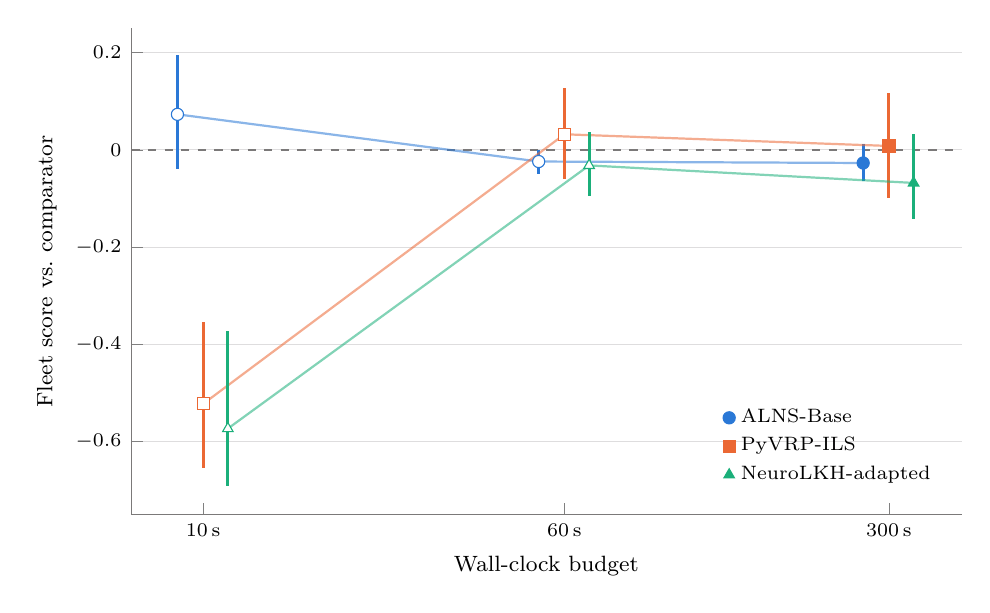
\begin{tikzpicture}
\begin{axis}[
  width=\columnwidth, height=0.64\columnwidth, xmode=log, xmin=7, xmax=430,
  xtick={10,60,300}, xticklabels={10\,s,60\,s,300\,s}, minor xtick={}, log ticks with fixed point,
  ymin=-0.75, ymax=0.25, ytick={-0.6,-0.4,-0.2,0,0.2}, yticklabel style={/pgf/number format/fixed},
  xlabel={Wall-clock budget}, ylabel={Fleet score vs.\ comparator},
  ymajorgrids, grid style={black!15}, axis lines*=left, axis line style={black!60},
  tick label style={font=\scriptsize}, label style={font=\footnotesize},
  mark size=2.2pt, error bars/error bar style={line width=1.1pt}, error bars/error mark=none,
  legend style={at={(0.98,0.04)}, anchor=south east, draw=none, fill=none, font=\scriptsize}, legend cell align=left,
]
\addplot[black!60, dashed, line width=0.6pt, forget plot] coordinates {(7,0) (430,0)};
% ALNS-Base
\addplot[cSerA, line width=0.8pt, opacity=0.55, forget plot] coordinates {(8.8,0.073) (52.8,-0.024) (264,-0.027)};
\addplot[cSerA, only marks, mark=*, mark options={fill=white}, forget plot, error bars/.cd, y dir=both, y explicit] coordinates {(8.8,0.073) += (0,0.121) -= (0,0.113) (52.8,-0.024) += (0,0.024) -= (0,0.025)};
\addplot[cSerA, only marks, mark=*, error bars/.cd, y dir=both, y explicit] coordinates {(264,-0.027) += (0,0.038) -= (0,0.037)};
\addlegendentry{ALNS-Base}
% PyVRP-ILS
\addplot[cSerB, line width=0.8pt, opacity=0.55, forget plot] coordinates {(10,-0.522) (60,0.032) (300,0.008)};
\addplot[cSerB, only marks, mark=square*, mark options={fill=white}, forget plot, error bars/.cd, y dir=both, y explicit] coordinates {(10,-0.522) += (0,0.168) -= (0,0.132) (60,0.032) += (0,0.095) -= (0,0.092)};
\addplot[cSerB, only marks, mark=square*, error bars/.cd, y dir=both, y explicit] coordinates {(300,0.008) += (0,0.109) -= (0,0.106)};
\addlegendentry{PyVRP-ILS}
% NeuroLKH-adapted
\addplot[cSerC, line width=0.8pt, opacity=0.55, forget plot] coordinates {(11.3,-0.573) (67.8,-0.032) (339,-0.068)};
\addplot[cSerC, only marks, mark=triangle*, mark options={fill=white}, forget plot, error bars/.cd, y dir=both, y explicit] coordinates {(11.3,-0.573) += (0,0.201) -= (0,0.117) (67.8,-0.032) += (0,0.069) -= (0,0.063)};
\addplot[cSerC, only marks, mark=triangle*, error bars/.cd, y dir=both, y explicit] coordinates {(339,-0.068) += (0,0.100) -= (0,0.075)};
\addlegendentry{NeuroLKH-adapted}
\end{axis}
\end{tikzpicture}
\caption{\DIFaddFL{Fleet score of the proposed configuration against each comparator by wall-clock budget. Positive values favor the proposed configuration. Filled markers at 300\,s show the confirmatory $98.33\%$ intervals; open markers at 10 and 60\,s show descriptive, unadjusted $95\%$ intervals. Markers are offset horizontally for legibility.}}
\label{fig:budget}
\end{figure}
\DIFaddend 

 \DIFaddbegin \DIFadd{Fig.~\ref{fig:budget} shows how the comparisons change with the budget. These results are descriptive and use unadjusted $95\%$ intervals. At 10\,s the proposed configuration used more vehicles than PyVRP-ILS ($-0.522$ }[\DIFadd{$-0.654$, $-0.354$}]\DIFadd{; 16 wins, 145 ties and 209 losses) and NeuroLKH-adapted ($-0.573$ }[\DIFadd{$-0.690$, $-0.372$}]\DIFadd{; 14, 130 and 226), and it did not differ detectably from ALNS-Base ($+0.073$ }[\DIFadd{$-0.040$, $0.194$}]\DIFadd{). At 60\,s it did not differ detectably from any of the three: $-0.024$ }[\DIFadd{$-0.049$, $0.000$}] \DIFadd{against ALNS-Base, $+0.032$ }[\DIFadd{$-0.060$, $0.128$}] \DIFadd{against PyVRP-ILS and $-0.032$ }[\DIFadd{$-0.095$, $0.036$}] \DIFadd{against NeuroLKH-adapted. The interval against ALNS-Base ends exactly at zero, so it does not show a difference. Where fleets matched at 60\,s, the distance gap against ALNS-Base was $+0.03\%$ }[\DIFadd{$-0.54$, $0.49$}]\DIFadd{. The other matched gaps at 10 and 60\,s have undefined intervals or no matched pairs and are given no direction.
}\DIFaddend 

 \DIFaddbegin \DIFadd{Compilation of the search kernels and the Guided Ejection Search phase are charged to the budget. In the 10\,s cells, the first improvement from any later phase came no earlier than 5.2\,s, with a median of 6.2, 6.3 and 7.3\,s at 100, 200 and 400 customers. In 123 of the 370 cells, no later phase improved on the solution the Guided Ejection Search phase left. Most of the first half of the budget therefore passed before the main search improved anything, so the 10\,s comparison says little about the search itself.
}

\DIFadd{The 900\,s stage was started and not completed, and no result from it is reported.
}

\subsection{Factorial Ablation (RQ3)}
\label{sec:ablation_results}
\DIFadd{The ablation uses 18 instances (the first instance of each of the six families at each size), five seeds, and budgets of 60 and 300\,s. Each of six factors (GEC, SP, Macro, Micro, LAC, GNN) is set to its low level in the full configuration and to its high level in the bare configuration. Low levels are not simple removals: GEC keeps direct insertion, SP disables every recombination query, Macro and Micro use rule-based policies in place of the DDQNs, LAC uses Simulated Annealing alone, and GNN runs without a heatmap. A $2\times2$ design contrasts the learning bundle (Macro, Micro, LAC, GNN) with the heuristic bundle (GEC, SP)}\DIFaddend . \DIFaddbegin \DIFadd{The case with all six factors low shares the search infrastructure, including the tail phases, and is not ALNS-Base. In the rerun the Guided Ejection Search phase is a fixed layer in all cases, so effects are measured on top of it.
}\DIFaddend 

 \DIFaddbegin \begin{table}[!t]
\DIFaddendFL \caption{ \DIFaddbeginFL \DIFaddFL{Factorial Ablation at 300\,s: Primary Contrasts }\DIFaddendFL ( \DIFaddbeginFL \DIFaddFL{Intervals at 99.38\%}\DIFaddendFL ) }
 \DIFaddbeginFL \label{tab:ablation}
\DIFaddendFL \centering
\scriptsize
 \DIFaddbeginFL \setlength{\tabcolsep}{3pt}
\begin{tabular}{l c c}
\DIFaddendFL \toprule
 \DIFaddbeginFL \DIFaddFL{\textbf{Contrast}} \DIFaddendFL &  \DIFaddbeginFL \DIFaddFL{\textbf{Fleet score}} \DIFaddendFL &  \DIFaddbeginFL \DIFaddFL{\textbf{Matched TD gap (\%)}} \DIFaddendFL \\
 \DIFaddbeginFL \midrule
\DIFaddFL{GEC full context }\DIFaddendFL &  \DIFaddbeginFL \DIFaddFL{$+0.000$ }[\DIFaddFL{$-0.110$, $0.072$}] \DIFaddendFL &  \DIFaddbeginFL \DIFaddFL{$-0.17$ }[\DIFaddFL{$-1.22$, $0.54$}] \DIFaddendFL \\
 \DIFaddbeginFL \DIFaddFL{SP full context }\DIFaddendFL &  \DIFaddbeginFL \DIFaddFL{$-0.044$ }[\DIFaddFL{$-0.181$, $0.067$}] \DIFaddendFL &  \DIFaddbeginFL \DIFaddFL{$+0.25$ }[\DIFaddFL{$-1.17$, $2.01$}] \DIFaddendFL \\
 \DIFaddbeginFL \DIFaddFL{Macro full context }\DIFaddendFL &  \DIFaddbeginFL \DIFaddFL{$-0.022$ }[\DIFaddFL{$-0.120$, $0.043$}] \DIFaddendFL &  \DIFaddbeginFL \DIFaddFL{$-0.27$ }[\DIFaddFL{$-1.60$, $0.71$}] \DIFaddendFL \\
 \DIFaddbeginFL \DIFaddFL{Micro full context }\DIFaddendFL &  \DIFaddbeginFL \DIFaddFL{$+0.044$ }[\DIFaddFL{$-0.095$, $0.201$}] \DIFaddendFL &  \DIFaddbeginFL \DIFaddFL{$-1.29$ }[\DIFaddFL{$-3.98$, $0.57$}] \DIFaddendFL \\
 \DIFaddbeginFL \DIFaddFL{LAC full context }\DIFaddendFL &  \DIFaddbeginFL \DIFaddFL{$-0.022$ }[\DIFaddFL{$-0.098$, $0.000$}] \DIFaddendFL &  \DIFaddbeginFL \DIFaddFL{$-0.32$ }[\DIFaddFL{$-1.08$, $0.22$}] \DIFaddendFL \\
 \DIFaddbeginFL \DIFaddFL{GNN full context }\DIFaddendFL &  \DIFaddbeginFL \DIFaddFL{$-0.044$ }[\DIFaddFL{$-0.167$, $0.067$}] \DIFaddendFL &  \DIFaddbeginFL \DIFaddFL{$+0.24$ }[\DIFaddFL{$-1.08$, $1.84$}] \DIFaddendFL \\
 \DIFaddbeginFL \DIFaddFL{heuristic at no learning }\DIFaddendFL &  \DIFaddbeginFL \DIFaddFL{$-0.044$ }[\DIFaddFL{$-0.216$, $0.067$}] \DIFaddendFL &  \DIFaddbeginFL \DIFaddFL{$+0.52$ }[\DIFaddFL{$-0.50$, $1.76$}] \DIFaddendFL \\
 \DIFaddbeginFL \DIFaddFL{learning at heuristic }\DIFaddendFL &  \DIFaddbeginFL \DIFaddFL{$+0.022$ }[\DIFaddFL{$-0.111$, $0.152$}] \DIFaddendFL &  \DIFaddbeginFL \DIFaddFL{$-0.08$ }[\DIFaddFL{$-1.55$, $1.86$}] \DIFaddendFL \\
 \DIFaddbeginFL \bottomrule
\end{tabular}

\vspace{2pt}
{\scriptsize \DIFaddFL{Positive fleet scores and negative gaps favor the component or bundle named. All 32 contrasts are in the supplement.}\par}
\end{table}

\DIFadd{Table~\ref{tab:ablation} gives the eight primary factorial contrasts at 300\,s. No primary factorial contrast excluded zero at 300\,s, so the ablation does not establish a benefit of the learned components at that budget. Most seed pairs tied, between 80 and 88 of the 90 in every primary contrast, and the point estimates ranged from $-0.044$ to $+0.044$. The learning bundle with the heuristic bundle present gave $+0.022$ }[\DIFadd{$-0.111$, $0.152$}]\DIFadd{, and Micro in the full context gave $+0.044$ }[\DIFadd{$-0.095$, $0.201$}]\DIFadd{.
}

\DIFadd{The LAC contrast is uninformative rather than evidence that LAC has no effect. Its fleet score was $-0.022$ }[\DIFadd{$-0.098$, $0.000$}]\DIFadd{, with no wins, 88 ties and }\DIFaddend 2  \DIFaddbegin \DIFadd{losses. In a separate one-seed measurement on the same 18 instances at 300\,s (Section~\ref{sec:cost_results}), LAC was consulted in 6 instances and passed its 300-decision warmup in 3, and its classifier did not approve a move in any of them. At this budget, acceptance therefore followed the Simulated Annealing rule throughout. The reason is the first search phase, in which LAC is not consulted (Section~\ref{sec:search_phases}). It ended in only those 6 instances: in }\DIFaddend 5  \DIFaddbegin \DIFadd{because the fleet reached the capacity bound, and in 1 at its iteration limit. In the other 12 the fleet stayed above the capacity bound, which serves as the floor when the Guided Ejection Search phase is on (Section~\ref{sec:setup}), so the stagnation exit did not apply, and the run ended before the limit of 6,000 iterations (1,028 to 5,194 iterations). This is a consequence of how that phase was added, not a property of LAC. We found the interaction after the rerun and did not change it, because the configuration was frozen. In the same measurement, the macro controller made no decision on the six R2 and RC2 instances.
}

\DIFadd{At 60\,s, on unadjusted $95\%$ intervals, three descriptive contrasts excluded zero: Micro in the bare configuration ($+0.344$ }[\DIFadd{$0.198$, $0.516$}]\DIFadd{), Micro in the full context ($+0.244$ }[\DIFadd{$0.053$, $0.492$}]\DIFadd{) and the learning bundle without the heuristic bundle ($+0.256$ }[\DIFadd{$0.114$, $0.433$}]\DIFadd{). They describe a pattern and do not establish one, and $47\%$ of the 60\,s ablation cells ran at a mean load above 8, measured with about one load sample per cell. At 300\,s, $56\%$ of ablation cells ran at a mean load above 8. No load repeat was fixed in advance for the ablation, so this exposure is reported but not adjusted for.
}

\DIFadd{The pattern for Micro-DDQN at 60\,s came from exploring results on the test set, so we tested it once more afterwards, under a protocol frozen before any cell ran. The size breakdown had been read first and motivated using 200 and 400 customers only. The test used Homberger instances 9 and 10 of each family at both sizes (24 instances), which are new time-window variants of the layouts of the ablation instances and not new layouts, with the four cases F111111, F111011, F000100 and F000000, five seeds and 60\,s; all 480 cells returned a valid solution. On the two confirmatory contrasts ($97.5\%$ intervals, sizes weighted equally), Micro-DDQN used fewer vehicles than the rule-based policy at 60\,s on these instances in the bare configuration ($+0.208$ }[\DIFadd{$0.025$, $0.450$}]\DIFadd{; 29 wins, 87 ties and }\DIFaddend 4  \DIFaddbegin \DIFadd{losses). In the full context the test did not detect a difference and is too small to rule one out ($+0.150$ }[\DIFadd{$-0.012$, $0.372$}]\DIFadd{; 25 wins, 88 ties and 7 losses). On descriptive $95\%$ intervals by size, the bare contrast was $+0.133$ }[\DIFadd{$-0.043$, $0.380$}] \DIFadd{at 200 customers and $+0.283$ }[\DIFadd{$0.029$, $0.640$}] \DIFadd{at 400, and the full-context contrast was $+0.083$ }[\DIFadd{$-0.080$, $0.386$}] \DIFadd{and $+0.217$ }[\DIFadd{$0.000$, $0.460$}]\DIFadd{. Where fleets matched, distance with Micro-DDQN was $11.7\%$ lower in the full context ($97.5\%$ interval }[\DIFadd{$-17.4\%$, $-7.3\%$}]\DIFadd{, 88 seed pairs) and $10.9\%$ lower in the bare configuration, where that interval is undefined. Of the 120 blocks, 71 ran at a mean load above 8; without them the fleet scores were $+0.114$ (bare) and $+0.157$ (full context) and both intervals are undefined, so we state no direction for those blocks alone. The test covers 200 and 400 customers at 60\,s and compares Micro-DDQN with a rule-based policy inside the same framework; it says nothing about 100 customers, about 300\,s, or about ALNS-Base, PyVRP-ILS and NeuroLKH-adapted, and the 300\,s results stand as reported.
}

\subsection{Instance Families (RQ5)}
\label{sec:family_results}

\DIFadd{By family, the comparisons are descriptive: they count the seed pairs in which the proposed configuration used fewer, the same or more vehicles than each comparator at 300\,s. The counts for every family and comparator are in Supplementary Section~8, with the per-instance means at each budget. On C1 and C2, every seed pair tied against all three comparators. Against ALNS-Base, the other four families were close, with 0 to }\DIFaddend 2  \DIFaddbegin \DIFadd{pairs fewer and 1 to }\DIFaddend 5  \DIFaddbegin \DIFadd{pairs more in each. Against PyVRP-ILS, the proposed configuration used fewer vehicles in }\DIFaddend 18  \DIFaddbegin \DIFadd{pairs and more in 1 on RC1, 10 and 10 on R1, 9 and 13 on R2, and none and 10 on RC2. Against NeuroLKH-adapted, the counts were 8 and 8 on R1, 8 and }\DIFaddend 2  \DIFaddbegin \DIFadd{on RC1, none and 21 on R2, and none and 10 on RC2. The losses therefore concentrate on R2 and RC2, the families with wide time windows: there the proposed configuration never used fewer vehicles than NeuroLKH-adapted, nor than PyVRP-ILS on RC2. Where fleets matched on R2 and RC2, its distance was 10.1\% and 15.4\% shorter than that of NeuroLKH-adapted, but no interval is computed per family, and under the lexicographic objective the fleet result comes first.
}\subsection{Availability and Feasibility}
\label{sec:feasibility_results}
\DIFadd{The supervisor validates every incumbent in the original problem space, checking customer coverage, capacity and time windows, before it counts. A cell without such an incumbent is reported as unavailable, and it is never replaced by a later or uncertified result. In the first sweep, 21 of the 8,620 cells were lost to infrastructure failures. In the rerun, all 8,060 cells of the five completed stages finished, so no comparison has an infrastructure gap. Five cells found no certified solution, all from comparators at short budgets: NeuroLKH-adapted on R1\_}\DIFaddend 4 \_\DIFaddbegin \DIFadd{1 (seeds 43 and 45) and RC1\_}\DIFaddend 4\_ \DIFaddbegin \DIFadd{1 (seed 45) at 10\,s, and PyVRP-ILS on RC1\_}\DIFaddend 4\_ \DIFaddbegin \DIFadd{1 (seed 42) at 10 and 60\,s. Every cell of the proposed configuration found one. Blocks with a cell frozen by machine sleep were moved aside unread and run again whole, 11 blocks with 74 cells, and 58 blocks at 300\,s (345 cells) were moved aside unread and rerun after load spikes on the machine. Of the }\DIFaddend 8 \DIFaddbegin \DIFadd{,060 cells, 350 returned more than 0.5\,s after their cutoff, 349 of them NeuroLKH-adapted (median 0.77\,s late, at most 1.20\,s), but in every cell the counted incumbent had been captured before the cutoff.
}

\subsection{Computational Cost}
\label{sec:cost_results}
\DIFadd{Each of the 18 ablation instances was run once more with the proposed configuration (seed 42, 300\,s), with timers on its main components. These runs measure shares of the budget, not solution quality. Each started at a one-minute load average of 3 or below, and four 400-customer runs ended at a load between }\DIFaddend 11  \DIFaddbegin \DIFadd{and 18. Set partitioning took the largest share, a median of $53\%$, $28\%$ and $22\%$ of the budget at 100, 200 and 400 customers. Destroy, repair and local search together took a median of $18\%$, $48\%$ and $50\%$, and the Guided Ejection Search phase took its allotted $10\%$. The learned controllers were cheap: macro, micro and LAC inference and training together took a median of $2.6\%$, $1.9\%$ and $0.8\%$, and at most $23\%$, on C101, where the main loop ran 213 iterations per second. GNN inference took $0.01\%$ and certification of incumbents less than $0.05\%$. About $11\%$ of the time was not attributed to a timed component. The main loop ran at a median of 17.8, 14.5 and 6.5 iterations per second at 100, 200 and 400 customers, counted over the whole run. The macro controller, which acts only at the start of a segment once the search has stagnated, made a median of 4.5 decisions per run: ten or fewer in 11 of the 18 runs, and none in 6. The compute of the learned layer is therefore unlikely to explain the null results above. The activity counts here and in Section~\ref{sec:ablation_results} suggest instead that parts of it rarely act at this budget.
}\DIFaddend 

 ALNS-Base  \DIFaddbegin \DIFadd{was not measured in this way, but the trajectories of the 300\,s cells give an estimate of its iteration rate. Between the first and the last improvement recorded in the main loop, }\DIFaddend ALNS-Base  \DIFaddbegin \DIFadd{ran at a median of about 662, 267 }\DIFaddend and  \DIFaddbegin \DIFadd{43 iterations per second at 100, 200 }\DIFaddend and  \DIFaddbegin \DIFadd{400 customers, against 23, 19 and 9 for the proposed configuration estimated the same way. That is about 28, 14 and 5 times as many, and 49 and 34 times as many on R2 and RC2. The estimate uses the 536 of 740 cells with two such improvements at least 5\,s apart. An iteration of the proposed configuration also carries local search and its share of set partitioning, so the two are not the same unit of work; the comparison shows how differently the two spend an equal budget.
}\DIFaddend 

\DIFaddbegin \subsection{Record of the First Sweep}
\label{sec:first_sweep}
\DIFadd{The first full sweep is kept on record. Its hybrid read the reference fleet, had no Guided Ejection Search phase, and ran under the varying machine speed described in Section~\ref{sec:setup}, so its results are valid within blocks and do not supersede the rerun.
}

\DIFaddend \begin{table*}[!t]
 \DIFaddbeginFL \caption{\DIFaddFL{First Sweep at 300\,s: F111111, Which Read the Reference Fleet, vs.\ Each Comparator (Intervals at 98.33\%)}}
\label{tab:first_sweep}
\DIFaddendFL \centering
\scriptsize
 \DIFaddbeginFL \setlength{\tabcolsep}{2pt}
\begin{tabular}{l c c c c}
\DIFaddendFL \toprule
 \DIFaddbeginFL \DIFaddFL{\textbf{Comparator}} \DIFaddendFL &  \DIFaddbeginFL \DIFaddFL{\textbf{Fleet score}} \DIFaddendFL &  \DIFaddbeginFL \makecell{\textbf{Seed pairs}\\\textbf{W/T/L}} \DIFaddendFL &  \DIFaddbeginFL \makecell{\textbf{Instances}\\\textbf{W/T/L}} \DIFaddendFL &  \DIFaddbeginFL \makecell{\textbf{Matched TD}\\\textbf{gap (\%)}} \DIFaddendFL \\
 \midrule
 \DIFaddbeginFL \DIFaddFL{ALNS-Base }\DIFaddendFL &  \DIFaddbeginFL \DIFaddFL{$+0.076$ }[\DIFaddFL{$-0.010$, $0.134$}] \DIFaddendFL &  \DIFaddbeginFL \DIFaddFL{38}\DIFaddendFL / \DIFaddbeginFL \DIFaddFL{320}\DIFaddendFL / \DIFaddbeginFL \DIFaddFL{10 }\DIFaddendFL &  \DIFaddbeginFL \DIFaddFL{16}\DIFaddendFL / \DIFaddbeginFL \DIFaddFL{54}\DIFaddendFL / \DIFaddbeginFL \DIFaddFL{4 }\DIFaddendFL &  \DIFaddbeginFL \DIFaddFL{$-0.23$ }[\DIFaddFL{$-0.65$, $0.11$}] \DIFaddendFL \\
 \DIFaddbeginFL \DIFaddFL{PyVRP-ILS }\DIFaddendFL &  \DIFaddbeginFL \DIFaddFL{$-0.065$ }[\DIFaddFL{$-0.183$, $0.083$}] \DIFaddendFL &  \DIFaddbeginFL \DIFaddFL{35}\DIFaddendFL / \DIFaddbeginFL \DIFaddFL{275}\DIFaddendFL / \DIFaddbeginFL \DIFaddFL{59 }\DIFaddendFL &  \DIFaddbeginFL \DIFaddFL{8}\DIFaddendFL / \DIFaddbeginFL \DIFaddFL{48/18 }\DIFaddendFL &  \DIFaddbeginFL \DIFaddFL{$+0.84$ (undefined) }\DIFaddendFL \\
 \DIFaddbeginFL \DIFaddFL{NeuroLKH-adapted }\DIFaddendFL & \DIFaddbeginFL \DIFaddFL{$-0.176$ }[\DIFaddFL{$-0.284$, $-0.029$}] \DIFaddendFL &  \DIFaddbeginFL \DIFaddFL{8/286/73 }\DIFaddendFL &  \DIFaddbeginFL \DIFaddFL{2/50/22 }\DIFaddendFL &  \DIFaddbeginFL \DIFaddFL{$-4.62$ (undefined) }\DIFaddendFL \\
 \bottomrule
 \DIFaddbeginFL \end{tabular}
\DIFaddendFL 

 \DIFaddbeginFL \vspace{2pt}
{\scriptsize \DIFaddFL{Instances W/T/L compares mean fleet over five seeds and is descriptive. Treating infrastructure gaps as failures changes no conclusion.}\DIFaddendFL \par}
\end{table*}

 \DIFaddbegin \DIFadd{Table~\ref{tab:first_sweep} shows that at 300\,s this hybrid did not differ detectably from ALNS-Base or PyVRP-ILS on fleet size and used more vehicles than NeuroLKH-adapted. Where fleets matched, the distance gap against NeuroLKH-adapted was $-4.62\%$, but that interval is undefined, so it is given no direction. Against PyVRP-ILS, no size stratum differed detectably: the fleet score was $-0.150$ at 100 customers, with a $95\%$ interval }[\DIFadd{$-0.257$, $0$}] \DIFadd{that ends at zero, and $+0.150$ and $+0.300$ at 200 and 400 customers, with intervals that include zero. At 10\,s it was behind all three comparators on fleet size. At 900\,s, on the unadjusted interval, it was ahead of ALNS-Base (fleet score $+0.135$}\DIFaddend ,  \DIFaddbegin [\DIFadd{$0.022$}\DIFaddend ,  \DIFaddbegin \DIFadd{$0.201$}]\DIFadd{; matched gap $-0.41\%$}\DIFaddend ,  \DIFaddbegin [\DIFadd{$-0.70$, $-0.03$}]\DIFadd{) and still behind NeuroLKH-adapted ($-0.134$, }[\DIFadd{$-0.224$, $-0.021$}]\DIFadd{)}\DIFaddend .

 \DIFaddbegin \DIFadd{In its factorial ablation, no primary contrast had a fleet interval excluding zero at 300\,s under the $99.38\%$ correction. On unadjusted intervals, the Micro DDQN against its rule policy in the full configuration ($+0.200$}\DIFaddend ,  \DIFaddbegin [\DIFadd{$0.060$}\DIFaddend ,  \DIFaddbegin \DIFadd{$0.366$}]\DIFadd{) and the learning bundle added to the heuristic bundle ($+0.189$}\DIFaddend ,  \DIFaddbegin [\DIFadd{$0.067$}\DIFaddend ,  \DIFaddbegin \DIFadd{$0.363$}]\DIFadd{) excluded zero at 60\,s, and the same contrast in the bare configuration did so at 300\,s ($+0.111$, }[\DIFadd{$0.022$}\DIFaddend ,  \DIFaddbegin \DIFadd{$0.178$}]\DIFadd{). The evidence for learned control in this sweep is therefore descriptive.
}\DIFaddend 

 \DIFaddbegin \section{Discussion}
\DIFaddend \label{sec:discussion}

This section interprets the  \DIFaddbegin \DIFadd{results, states their practical meaning, and lists the limitations of the method and of the evidence.
}\DIFaddend 

 \DIFaddbegin \subsection{Where the Method Does and Does Not Help}
\DIFaddend \label{sec:disc_scale_aware}
 \DIFaddbegin \DIFadd{Against ALNS-Base, the proposed configuration gained nothing detectable on fleet size at any budget: the intervals at 10, 60 }\DIFaddend and  \DIFaddbegin \DIFadd{300\,s all contain zero or end at it, and most seed pairs tied. This comparison does not isolate the learned layer, because ALNS-Base also lacks the local search, ejection chains and set partitioning of the hybrid; the ablation is the comparison that does}\DIFaddend .

 \DIFaddbegin \DIFadd{Against PyVRP-ILS and NeuroLKH-adapted, it did not differ detectably at 300\,s or 60\,s, and at 10\,s it used more vehicles than both on unadjusted intervals; compilation and the Guided Ejection Search phase take most of the first half of that budget. By family, the losses concentrate on R2 and RC2, the families with wide time windows: there it never used fewer vehicles than NeuroLKH-adapted, nor than PyVRP-ILS on RC2. It used fewer vehicles than PyVRP-ILS in 18 seed pairs and more in 1 on RC1, which is descriptive and does not establish an advantage.
}

\DIFadd{The classical Guided Ejection Search phase matters more to ALNS-Base than to the hybrid: at 300\,s, with the phase against without it, }\DIFaddend the  \DIFaddbegin \DIFadd{fleet score was $+0.208$ for ALNS-Base but only $+0.062$ for the hybrid. On descriptive $95\%$ intervals, ALNS-Base with the phase used fewer vehicles than without it ($+0.208$ }[\DIFadd{$0.052$, $0.291$}]\DIFadd{; 80 wins, 287 ties and 3 losses). Without the phase, the hybrid used fewer vehicles than ALNS-Base ($+0.116$ }[\DIFadd{$0.002$, $0.181$}]\DIFadd{) and more than NeuroLKH-adapted ($-0.135$ }[\DIFadd{$-0.236$, $-0.012$}]\DIFadd{); with the phase on both, the difference from ALNS-Base was no longer detectable. The hybrid's other classical components differ from ALNS-Base as well, so even the comparison without the phase is not evidence for learned control.
}

\DIFadd{The trajectories show where the fleet size is decided. In 338 of the 370 seed pairs at 300\,s, the hybrid and ALNS-Base had the same fleet size both right after the Guided Ejection Search phase and at the end. Right after the phase, the hybrid had the larger fleet in 11 pairs and the smaller one in 11. After it, the fleet was reduced further in only 46 runs of the hybrid and 50 of ALNS-Base. Of the 14 pairs the hybrid lost, 5 were already behind after the phase, and the other 9 were on R2 and RC2 instances, where ALNS-Base removed more vehicles afterwards than the hybrid did. At this budget the fleet size is therefore largely set by the classical phase, which leaves the main loop, learned or not, little to gain. ALNS-Base also completes many more main-loop iterations in the same time (Section~\ref{sec:cost_results}), most of all on R2 and RC2, which is consistent with its removing more vehicles there after the phase. These counts are descriptive.
}

\DIFadd{The ablation does not establish a benefit of the learned components at 300\,s. At that budget the LAC classifier never changed an acceptance decision and the macro controller made no decision on the R2 and RC2 instances, so parts of the learned layer were hardly exercised; the LAC contrast is uninformative, not a null effect. The one signal for learning concerns }\DIFaddend Micro-DDQN  \DIFaddbegin \DIFadd{at 60\,s. In a separate test on new time-window variants of the same layouts, it used fewer vehicles than the rule-based policy in the bare configuration, the test did not detect a difference in the full context, and the bare result is not confirmed without the blocks run at high load (Section~\ref{sec:ablation_results}). These conclusions concern the 74 benchmark instances, the 24 time-window variants of the Micro test, the budgets and the single machine of this study, and do not extend beyond them.
}\DIFaddend 

\subsection{Managerial Implications for Commercial Logistics}
\label{sec:disc_managerial}

In commercial freight operations, capital depreciation, vehicle financing, insurance, and driver shift wages dominate marginal fuel consumption \cite{Toth2014, braysy2005vehicle}. Fixed vehicle  \DIFaddbegin \DIFadd{cost is therefore the main driver, and removing one vehicle saves more, and more regularly, than a marginal distance improvement. Extra compute is therefore worth spending when it removes a vehicle, but the solver that removes it need not be this one. At a planning budget of 5 minutes, the results do not favor a solver on fleet size: none of the three comparators differed detectably from the proposed configuration at 300\,s. The choice therefore cannot rest on these results, and the simplest solver to deploy and maintain is a reasonable default; the proposed method adds learned controllers whose benefit this study does not establish. For budgets of seconds, PyVRP-ILS }\DIFaddend and  \DIFaddbegin \DIFadd{NeuroLKH-adapted used fewer vehicles than the proposed configuration at 10\,s on unadjusted intervals. No 900\,s result is reported, so the study gives no guidance for a 15-minute budget}\DIFaddend .

 \subsection{Limitations and Threats to Validity}
\label{sec:disc_limitations}
The  \DIFaddbegin \DIFadd{main limitations are these. }\DIFaddend (i)  \DIFaddbegin \DIFadd{Benchmark Scope: the evaluation covers 74 instances with four geometry groups per size and few large instances, so it says little about other distributions. }\DIFaddend (ii) MIP Dependency: Set Partitioning relies on  \DIFaddbegin \DIFadd{HiGHS throughput within a per-query time limit. }\DIFaddend (iii) Compute Overhead:  \DIFaddbegin \DIFadd{online neural updates and Set Partitioning consume part of each }\DIFaddend wall-clock  \DIFaddbegin \DIFadd{budget that would otherwise go to search iterations. }\DIFaddend (iv) Static Scope:  \DIFaddbegin \DIFadd{the }\DIFaddend framework targets static VRPTW \DIFaddbegin \DIFadd{. }\DIFaddend (v) GNN Scale Shift:  \DIFaddbegin \DIFadd{the GNN was trained and validated with one training seed at }\DIFaddend $N=100$  \DIFaddbegin \DIFadd{and $200$ only, so use at }\DIFaddend $N=400$  \DIFaddbegin \DIFadd{is an extrapolation, and its validation recall is measured against heuristic labels. }\DIFaddend (vi) LAC  \DIFaddbegin \DIFadd{Not Exercised: in the cost measurement at 300\,s, the LAC classifier never changed an acceptance decision, so these experiments do not test LAC. In 12 of the 18 instances it was not consulted at all, because the first search phase did not end there (Section~\ref{sec:ablation_results}). Because it }\DIFaddend operates disjunctively ($\text{Accept} \iff p_t \ge \tau_{\text{acc}} \lor P_{\text{SA}} > U$),  \DIFaddbegin \DIFadd{separating predictive lookahead from a higher acceptance rate would also need budgets or instances where it fires. (vii) Effective Compute: machine speed varied between blocks of cells (Section~\ref{sec:setup}), so results are comparable within a block and do not describe a fixed amount of compute. (viii) One Machine and Fixed Baseline Settings: all runs used one notebook, and the baselines were not tuned for these budgets. (ix) Test-Informed Development: test results motivated the Guided Ejection Search phase, and the development instances share coordinates with test instances (Section~\ref{sec:setup}). Every incumbent counted in the results is validated in the original problem space by the supervisor before it counts, and cells without a valid incumbent are reported as unavailable.
}\DIFaddend 

\section{Conclusion}
\label{sec:conclusion}
This paper  \DIFaddbegin \DIFadd{asked whether learned control inside ALNS pays for its compute when the controllers start from random weights in every run. The test case was }\DIFaddend Tri-Level Hybrid DDQN-ALNS,  \DIFaddbegin \DIFadd{which adds a macro plateau controller, a micro operator controller and a learned acceptance criterion to ALNS, and every solution counted was validated in the original problem space.
}\DIFaddend 

 \DIFaddbegin \DIFadd{At 300\,s, the proposed configuration did not differ detectably on fleet size from ALNS-Base, PyVRP-ILS or NeuroLKH-adapted, and no primary factorial contrast excluded zero, so this study does not establish a benefit of the learned components at that budget. One detectable gain, from the classical Guided Ejection Search phase, was small and did not survive leaving out blocks run at high machine load. A second concerns a learned component: at 60\,s, in a separate test on new time-window variants at 200 and 400 customers, Micro-DDQN used fewer vehicles than the rule-based policy in the bare configuration, while the test did not detect a difference in the full context; without the blocks run at high load, neither interval is defined. On descriptive intervals, the proposed configuration used more vehicles than PyVRP-ILS and NeuroLKH-adapted at 10\,s, and on the wide-time-window families R2 and RC2 it never used fewer vehicles than NeuroLKH-adapted.
}

\DIFadd{At 300\,s, the learned acceptance criterion never changed an acceptance decision and the macro controller was idle on R2 and RC2, so the value of these components remains untested rather than refuted. A test of them needs conditions under which they act, which longer budgets or controllers trained before the run might provide; whether they would help there is open. The }\DIFaddend benchmark instances,  \DIFaddbegin \DIFadd{the GNN checkpoint, the solver and baseline adapter code, the }\DIFaddend evaluation scripts, and  \DIFaddbegin \DIFadd{compact records of the rerun and of the Micro test (the validated fleet size, distance, timing and load of every cell in the reported stages, together with the analysis outputs and the frozen solver snapshot) }\DIFaddend are available at  \DIFaddbegin \url{https://github.com/Thundercok/vrptw-neural-hybrid-optimizer}\DIFadd{. The full per-cell outputs, about 23\,GB, are available from the authors on request.
}\section*{\DIFadd{Acknowledgment}}
\DIFadd{The authors used Claude (Anthropic) to write analysis and experiment code, to generate the result tables and Figs.~\ref{fig:architecture} and~\ref{fig:budget}, to edit the wording of the manuscript, and to draft parts of the abstract, the introduction and Sections~\ref{sec:formulation}--\ref{sec:conclusion}, which the authors reviewed and revised. The authors verified all output against the experimental records and take full responsibility for the content.
}\DIFaddend 

{\footnotesize
\begin{thebibliography}{10}
\setlength{\itemsep}{-3.8pt}
\setlength{\parskip}{0pt}
\providecommand{\url}[1]{#1}
\csname url@samestyle\endcsname
\providecommand{\newblock}{\relax}
\providecommand{\bibinfo}[2]{#2}
\providecommand{\BIBentrySTDinterwordspacing}{\spaceskip=0pt\relax}
\providecommand{\BIBentryALTinterwordstretchfactor}{4}
\providecommand{\BIBentryALTinterwordspacing}{\spaceskip=\fontdimen2\font plus
\BIBentryALTinterwordstretchfactor\fontdimen3\font minus \fontdimen4\font\relax}
\providecommand{\BIBforeignlanguage}[2]{{%
\expandafter\ifx\csname l@#1\endcsname\relax
\typeout{** WARNING: IEEEtran.bst: No hyphenation pattern has been}%
\typeout{** loaded for the language `#1'. Using the pattern for}%
\typeout{** the default language instead.}%
\else
\language=\csname l@#1\endcsname
\fi
#2}}
\providecommand{\BIBdecl}{\relax}
\BIBdecl

\bibitem{Dantzig1959}
G.~B. Dantzig and J.~H. Ramser, ``The truck dispatching problem,'' \emph{Management Science}, vol.~6, no.~1, pp. 80--91, 1959.

\bibitem{Solomon1987}
M.~M. Solomon, ``Algorithms for the vehicle routing and scheduling problems with time window constraints,'' \emph{Operations Research}, vol.~35, no.~2, pp. 254--265, 1987.

\bibitem{Toth2014}
P.~Toth and D.~Vigo, Eds., \emph{Vehicle Routing: Problems, Methods, and Applications}, 2nd~ed.\hskip 1em plus 0.5em minus 0.4em\relax Philadelphia, PA, USA: SIAM, 2014.

\bibitem{braysy2005vehicle}
O.~Br{\"a}ysy and M.~Gendreau, ``Vehicle routing problem with time windows, part  \DIFaddbegin {\DIFadd{I}}\DIFaddend : Route construction and local search algorithms,'' \emph{Transportation Science}, vol.~39, no.~1, pp. 104--118, 2005.

\DIFaddbegin \bibitem{pisinger2007general}
\DIFadd{D.~Pisinger and S.~Ropke, ``A general heuristic for vehicle routing problems,'' }\emph{\DIFadd{Computers \& Operations Research}}\DIFadd{, vol.~34, no.~8, pp. 2403--2435, 2007.
}

\DIFaddend \bibitem{Ropke2006}
S.~Ropke and D.~Pisinger, ``An adaptive large neighborhood search heuristic for the pickup and delivery problem with time windows,'' \emph{Transportation Science}, vol.~40, no.~4, pp. 455--472, 2006.

 \DIFaddbegin \bibitem{kallestad2023general}
\DIFadd{J.~Kallestad, R.~Hasibi, A.~Hemmati, and K.~S}{\DIFadd{\"o}}\DIFadd{rensen}\DIFaddend , ``A general  \DIFaddbegin \DIFadd{deep reinforcement learning hyperheuristic framework for solving combinatorial optimization }\DIFaddend problems,'' \emph{ \DIFaddbegin \DIFadd{European Journal of Operational }\DIFaddend Research}, vol.~ \DIFaddbegin \DIFadd{309}\DIFaddend , no.~ \DIFaddbegin \DIFadd{1}\DIFaddend , pp.  \DIFaddbegin \DIFadd{446--468, 2023.
}\DIFaddend 

\DIFaddbegin \bibitem{johnn2023graph}
\DIFadd{S.~N. Johnn, V.-A. Darvariu, J.~Handl, and J.~Kalcsics, ``Graph reinforcement learning for operator selection in the }{\DIFadd{ALNS}} \DIFadd{metaheuristic,'' in }\emph{\DIFadd{Optimization and Learning (OLA 2023)}}\DIFadd{, Cham, Switzerland: Springer, 2023, pp. 200--212.
}

\bibitem{reijnen2024online}
\DIFadd{R.~Reijnen, Y.~Zhang, H.~C. Lau, and Z.~Bukhsh, ``Online control of adaptive large neighborhood search using deep reinforcement learning,'' in }\emph{\DIFadd{Proc. Int. Conf. Automated Planning and Scheduling}}\DIFadd{, vol.~34, no.~1, 2024, pp. 475--483.
}

\DIFaddend \bibitem{vinyals2015pointer}
O.~Vinyals, M.~Fortunato, and N.~Jaitly, ``Pointer networks,'' in \emph{Advances in  \DIFaddbegin \DIFadd{Neural Information Processing Systems}\DIFaddend }, vol.~28, 2015, pp. 2692--2700.

\bibitem{kool2019attention}
W.~Kool, H.~van Hoof, and M.~Welling, ``Attention, learn to solve routing problems!'' in \emph{International Conference on Learning Representations (ICLR)}, 2019.

\bibitem{nazari2018reinforcement}
M.~Nazari, A.~Oroojlooy, L.~V. Snyder, and M.~Tak{\'a}{\v{c}}, ``Reinforcement learning for solving the vehicle routing problem,'' in \emph{Advances in  \DIFaddbegin \DIFadd{Neural Information Processing Systems}\DIFaddend }, \DIFaddbegin \DIFadd{vol.~31, }\DIFaddend 2018, pp. 9861--9871.

\bibitem{falkner2020learning}
J.~K. Falkner and L.~Schmidt-Thieme, ``Learning to solve vehicle routing problems with time windows through joint attention,'' \emph{arXiv preprint arXiv:2006.09100}, 2020.

\bibitem{lin2021deep}
B.~Lin, B.~Ghaddar, and J.~Nathwani, ``Deep reinforcement learning for the electric vehicle routing problem with time windows,'' \emph{IEEE Transactions on Intelligent Transportation Systems}, vol.~23, no.~8, pp. 11\,528--11\,538, 2022.

\bibitem{christiaens2020slack}
J.~Christiaens and G.~Vanden~Berghe, ``Slack induction by string removals for vehicle routing problems,'' \emph{Transportation Science}, vol.~54, no.~2, pp. 417--433, 2020.

\bibitem{vidal2013hybrid}
T.~Vidal, T.~G. Crainic, M.~Gendreau, and  \DIFaddbegin \DIFadd{C.~}\DIFaddend Prins, ``A hybrid genetic algorithm with adaptive diversity management for a large class of vehicle routing problems with time-windows,'' \emph{Computers \& Operations Research}, vol.~40, no.~1, pp. 475--489, 2013.

\bibitem{lu2020learning}
H.~Lu, X.~Zhang, and S.~Yang, ``A learning-based iterative  \DIFaddbegin \DIFadd{method for solving vehicle routing problems,'' in }\DIFaddend \emph{ \DIFaddbegin \DIFadd{International Conference }\DIFaddend on  Learning  \DIFaddbegin \DIFadd{Representations (ICLR)}\DIFaddend },  2020.

\bibitem{hottung2020neural}
A.~Hottung and K.~Tierney, ``Neural large neighborhood search for the capacitated vehicle routing problem,'' in \emph{Proc. 24th European Conference on Artificial Intelligence (ECAI)}, 2020, pp. 443--450.

\bibitem{shaw1998using}
P.~Shaw, ``Using constraint programming and local search methods to solve vehicle routing problems,'' in \emph{Proc. CP 1998}, ser. LNCS, vol. 1520.\hskip 1em plus 0.5em minus 0.4em\relax Springer, 1998, pp. 417--431.

\bibitem{pisinger2010large}
D.~Pisinger and S.~Ropke, ``Large neighborhood search,'' in \emph{Handbook of Metaheuristics}.\hskip 1em plus 0.5em minus 0.4em\relax Springer, 2010, pp. 399--419.

\bibitem{nagata2009ges}
Y.~Nagata and O.~Br{\"a}ysy, ``A powerful route minimization heuristic for the vehicle routing problem with time windows,'' \emph{Operations Research Letters}, vol.~37, no.~5, pp. 333--338, 2009.

\bibitem{nagata2010srex}
Y.~Nagata, O.~Br{\"a}ysy, and W.~Dullaert, ``A penalty-based edge assembly memetic algorithm for the vehicle routing problem with time windows,'' \emph{Computers \& Operations Research}, vol.~37, no.~4, pp. 724--737, 2010.

\bibitem{rochat1995probabilistic}
Y.~Rochat and {\'E}.~D. Taillard, ``Probabilistic diversification and  \DIFaddbegin \DIFadd{intensification }\DIFaddend in local search for vehicle routing,'' \emph{Journal of Heuristics}, vol.~1, no.~1, pp. 147--167, 1995.

\bibitem{alvarenga2007genetic}
G.~ \DIFaddbegin \DIFadd{B}\DIFaddend . Alvarenga, G.~R. Mateus, and G.~de~ \DIFaddbegin \DIFadd{Tomi}\DIFaddend , ``A genetic and set partitioning \DIFaddbegin \DIFadd{two-phase }\DIFaddend approach for the vehicle routing problem with time windows,'' \emph{Computers \& Operations Research}, vol.~34, no.~ \DIFaddbegin \DIFadd{6}\DIFaddend , pp.  \DIFaddbegin \DIFadd{1561--1584}\DIFaddend , 2007.

\bibitem{subramanian2013hybrid}
A.~Subramanian,  E.~Uchoa, and L.~S. Ochi, ``A hybrid algorithm for  \DIFaddbegin \DIFadd{a class of vehicle routing problems}\DIFaddend ,'' \emph{Computers \& Operations Research}, vol.~40, no.~ \DIFaddbegin \DIFadd{10}\DIFaddend , pp.  \DIFaddbegin \DIFadd{2519--2531}\DIFaddend , 2013.

\bibitem{turkes2021meta}
R.~Turke{\v{s}}, K.~S{\"o}rensen, and L.~M. Hvattum, ``Meta-analysis of \DIFaddbegin \DIFadd{metaheuristics: Quantifying the effect of adaptiveness in }\DIFaddend adaptive large neighborhood search,'' \emph{European Journal of Operational Research}, vol. 292, no.~2, pp. 423--442, 2021.

\bibitem{bello2016neural}
I.~Bello, H.~Pham, Q.~V. Le, M.~Norouzi, and S.~Bengio, ``Neural combinatorial optimization with reinforcement learning,'' \emph{arXiv preprint arXiv:1611.09940}, 2016.

\bibitem{khalil2017learning}
E.~Khalil, H.~Dai, Y.~Zhang, B.~Dilkina, and L.~Song, ``Learning combinatorial optimization algorithms over graphs,'' in \emph{Advances in  \DIFaddbegin \DIFadd{Neural Information Processing Systems}\DIFaddend }, vol.~30, 2017, pp. 6348--6358.

\bibitem{joshi2019efficient}
C.~K. Joshi, T.~Laurent, and X.~Bresson, ``An efficient graph convolutional network technique for the travelling salesman problem,'' \emph{arXiv preprint arXiv:1906.01227}, 2019.

\bibitem{bengio2021machine}
Y.~Bengio, A.~Lodi, and Y.~Prouvost, ``Machine learning for combinatorial optimization: A methodological tour d'horizon,'' \emph{European Journal of Operational Research}, vol. 290, no.~2, pp. 405--421, 2021.

 \bibitem{chen2019learning}
X.~Chen and Y.~Tian, `` \DIFaddbegin \DIFadd{Learning to perform local rewriting for combinatorial optimization,'' }\DIFaddend in \emph{Advances in  \DIFaddbegin \DIFadd{Neural Information Processing Systems}}\DIFadd{, vol.~32, 2019, pp. 6281--6292.
}

\bibitem{sutton1999between}
\DIFadd{R.~S. Sutton, D.~Precup, and S.~Singh, ``Between MDPs and semi-MDPs: A framework for temporal abstraction in reinforcement learning,'' }\emph{\DIFadd{Artificial Intelligence}\DIFaddend }, vol.  \DIFaddbegin \DIFadd{112, no.~1-2, pp. 181--211, 1999.
}

\bibitem{mnih2015human}
\DIFadd{V.~Mnih }\emph{\DIFadd{et~al.}}\DIFadd{, ``Human-level control through deep reinforcement learning,'' }\emph{\DIFadd{Nature}}\DIFadd{, vol.~518, no.~7540, pp. 529--533, 2015.
}

\bibitem{vanhasselt2016deep}
\DIFadd{H.~van Hasselt, A.~Guez, and D.~Silver, ``Deep reinforcement learning with double }{\DIFadd{Q}}\DIFadd{-learning,'' in }\emph{\DIFadd{Proc. 30th AAAI Conf. Artificial Intelligence}}\DIFadd{, 2016, pp. 2094--2100}\DIFaddend .

\DIFaddbegin \bibitem{schaul2016prioritized}
\DIFadd{T.~Schaul, J.~Quan, I.~Antonoglou, and D.~Silver, ``Prioritized experience replay,'' in }\emph{\DIFadd{International Conference on Learning Representations (ICLR)}}\DIFadd{, 2016.
}

\bibitem{li2006unified}
\DIFadd{L.~Li, T.~J. Walsh, and M.~L. Littman, ``Towards a unified theory of state abstraction for }{\DIFadd{MDPs}}\DIFadd{,'' in }\emph{\DIFadd{Proc. 9th Int. Symp. Artificial Intelligence and Mathematics (ISAIM)}}\DIFadd{, 2006, pp. 531--539.
}

\DIFaddend \bibitem{ng1999policy}
A.~Y. Ng, D.~Harada, and S.~Russell, ``Policy invariance under reward transformations: Theory and application to reward shaping,'' in \emph{Proc. 16th ICML}, 1999, pp. 278--287.

\bibitem{wang2016dueling}
Z.~Wang \emph{et~al.}, ``Dueling network architectures for deep reinforcement learning,'' in \emph{Proc. 33rd ICML}, vol.~48, 2016, pp. 1995--2003.

 \DIFaddbegin \bibitem{auer2002finite}
\DIFadd{P.~Auer, N.~Cesa-Bianchi, and P.~Fischer, ``Finite-time analysis of the multiarmed bandit problem,'' }\emph{\DIFadd{Machine Learning}}\DIFadd{, vol.~47, no.~2--3, pp. 235--256, 2002.
}

\bibitem{audibert2009exploration}
\DIFadd{J.-Y.~Audibert, R.~Munos, and C.~Szepesv}{\DIFadd{\'a}}\DIFadd{ri, ``Exploration--exploitation tradeoff using variance estimates in multi-armed bandits,'' }\DIFaddend \emph{ \DIFaddbegin \DIFadd{Theoretical Computer Science}\DIFaddend }, vol.  \DIFaddbegin \DIFadd{410, no.~19, pp. 1876--1902, 2009.
}

\bibitem{hajek1988cooling}
\DIFadd{B.~Hajek, ``Cooling schedules for optimal annealing,'' }\emph{\DIFadd{Mathematics of Operations Research}}\DIFadd{, vol.~13, }\DIFaddend no.~ \DIFaddbegin \DIFadd{2}\DIFaddend , pp.  \DIFaddbegin \DIFadd{311--329, 1988.
}\DIFaddend 

\bibitem{savelsbergh1992general}
M.~W. Savelsbergh, ``The vehicle routing problem with time windows: Minimizing route duration,'' \emph{ORSA Journal on Computing}, vol.~4, no.~2, pp. 146--154, 1992.

\bibitem{toth2003granular}
P.~Toth and D.~Vigo, ``The granular tabu search and its application to the vehicle-routing problem,'' \emph{INFORMS Journal on Computing}, vol.~15, no.~4, pp. 333--346, 2003.

\DIFaddbegin \bibitem{huangfu2018parallelizing}
\DIFadd{Q.~Huangfu and J.~A.~J. Hall, ``Parallelizing the dual revised simplex method,'' }\emph{\DIFadd{Mathematical Programming Computation}}\DIFadd{, vol.~10, no.~1, pp. 119--142, 2018.
}

\DIFaddend \bibitem{gehring1999parallel}
H.~Gehring and J.~Homberger, ``A parallel hybrid evolutionary metaheuristic for the vehicle routing problem with time windows,'' in \emph{Proc. EUROGEN99}, K.~Miettinen, M.~M.~M{\"a}kel{\"a}, and J.~Toivanen, Eds. University of Jyv{\"a}skyl{\"a}, Finland, 1999, pp. 57--64.

 \DIFaddbegin \bibitem{wouda2024pyvrp}
\DIFadd{N.~A. Wouda, L.~Lan, and W.~Kool, ``}\DIFaddend { \DIFaddbegin \DIFadd{PyVRP}\DIFaddend } \DIFaddbegin \DIFadd{: A high-performance }{\DIFadd{VRP}} \DIFadd{solver package,'' }\DIFaddend \emph{ \DIFaddbegin \DIFadd{INFORMS Journal on Computing}\DIFaddend }, vol.~ \DIFaddbegin \DIFadd{36}\DIFaddend , no.~ \DIFaddbegin \DIFadd{4}\DIFaddend , pp.  \DIFaddbegin \DIFadd{943--955, 2024.
}\DIFaddend 

 \DIFaddbegin \bibitem{xin2021neurolkh}
\DIFadd{L.~Xin, W.~Song, Z.~Cao, and J.~Zhang, ``}{\DIFadd{NeuroLKH}}\DIFadd{: Combining deep learning model with }{\DIFadd{Lin-Kernighan-Helsgaun}} \DIFadd{heuristic for solving the traveling salesman problem}\DIFaddend , '' in \emph{ \DIFaddbegin \DIFadd{Advances in Neural Information Processing Systems}\DIFaddend },  \DIFaddbegin \DIFadd{vol.~34, 2021, pp. 7472--7483.
}\DIFaddend 

 \bibitem{sintef_homberger}
{SINTEF Optimization}, ``{SINTEF} {VRPTW} benchmark portal: Best known solutions for Homberger extended instances,'' \url{https://www.sintef.no/projectweb/top/vrptw/homberger-benchmark/}, 2024.
 \end{thebibliography}
}

 \DIFaddbegin \newpage
\DIFaddend \phantomsection
\begin{IEEEbiography}[{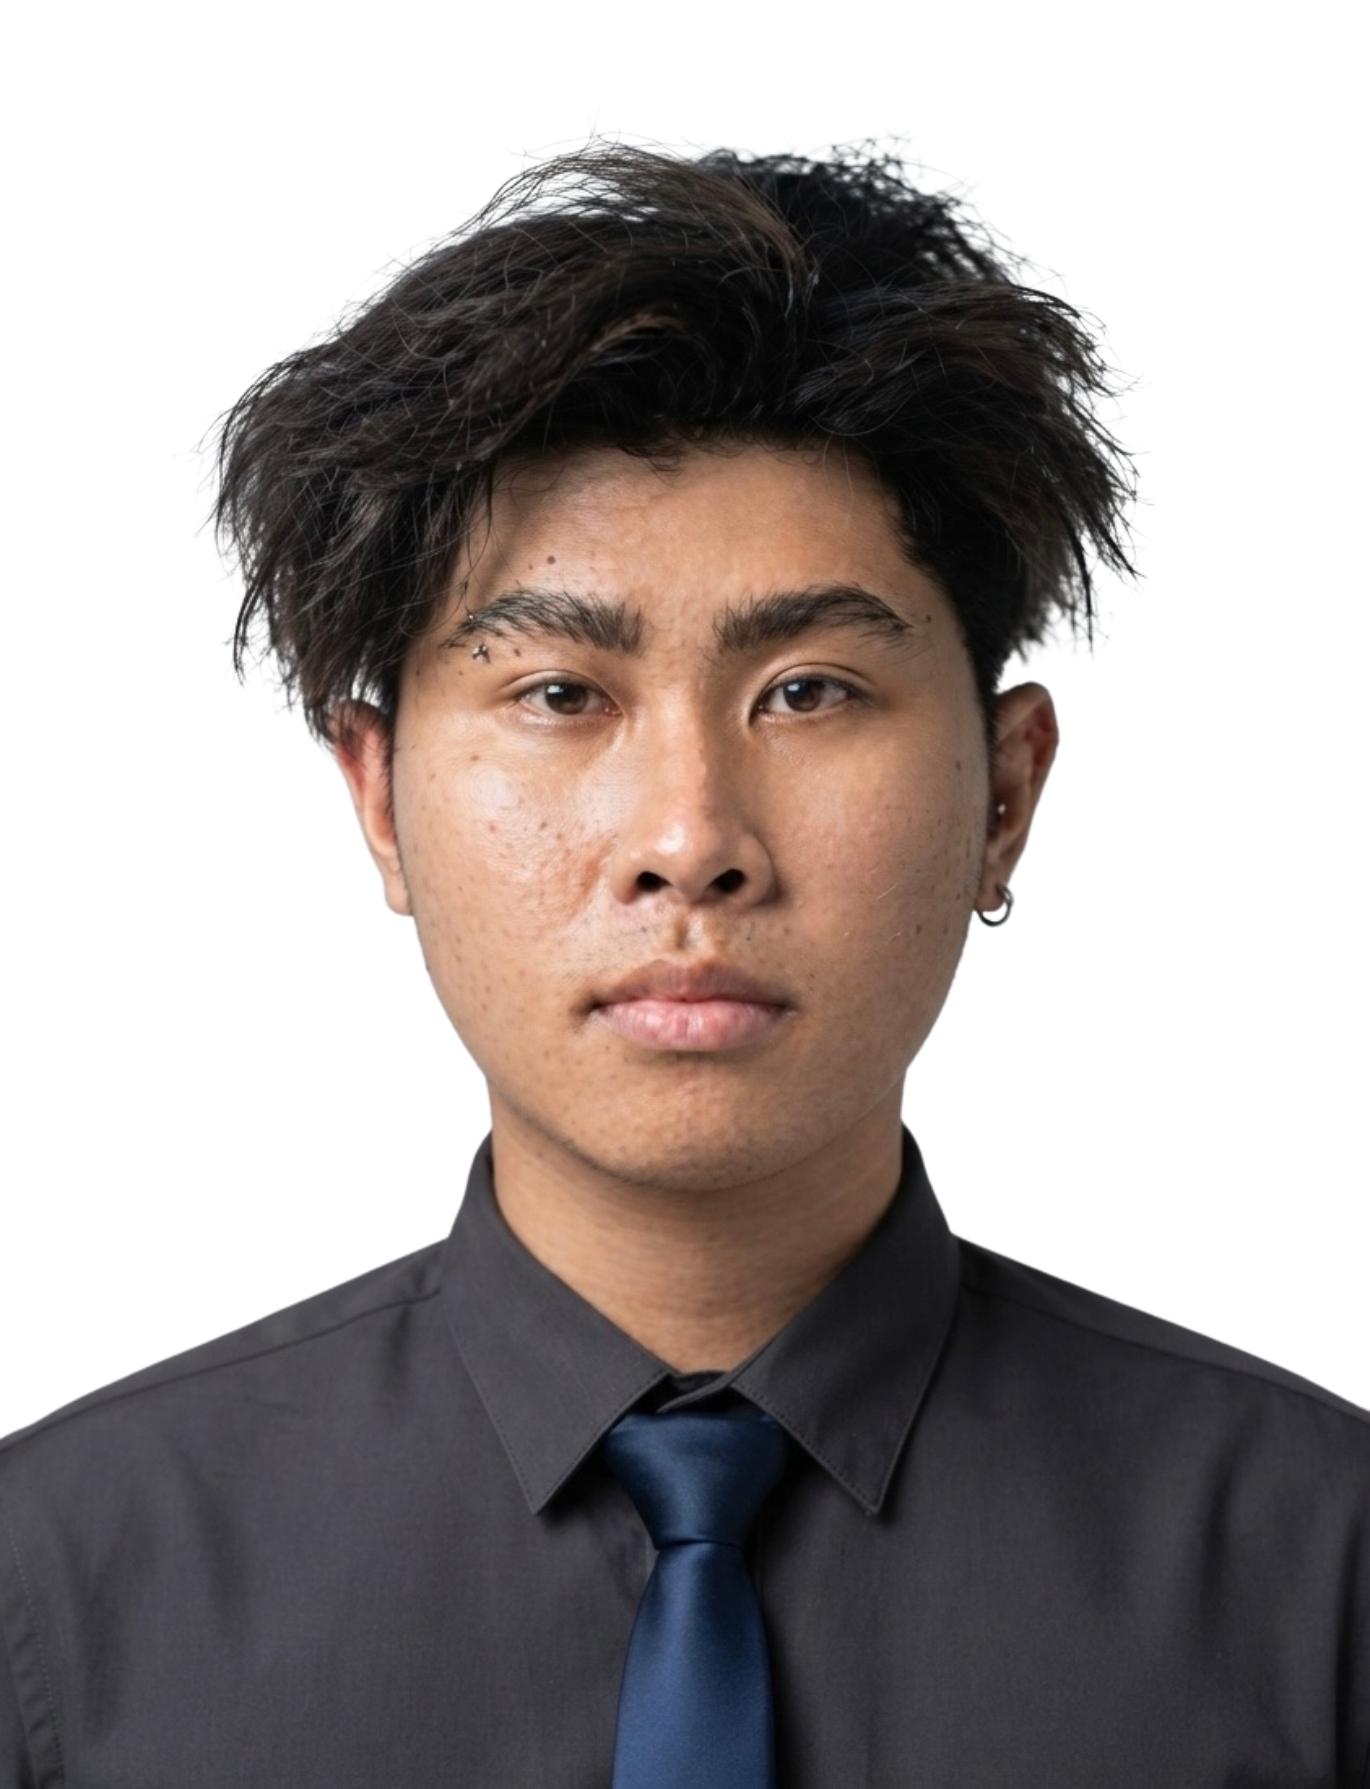
\includegraphics[width=1.0in,height=1.25in,clip,keepaspectratio]{profile_Huy.jpg}}]{Huynh Nhat Huy} is currently pursuing the B.S. degree in Computer Science with the Faculty of Information Technology, Ton Duc Thang University, Ho Chi Minh City, Vietnam. His research interests include deep reinforcement learning, combinatorial optimization, metaheuristics, and learning-augmented algorithms.
\end{IEEEbiography}

\begin{IEEEbiography}[{
\includegraphics[width=1.0in,height=1.25in,clip,keepaspectratio]{fig6_profileho.jpg}}]{Thi-Linh Ho} received the B.S. degree from Nong Lam University in 2009, the M.S. degree from Ho Chi Minh City University of Technology in 2012, and the Ph.D. degree in Computer Science from Ton Duc Thang University, Vietnam, in 2024. She is currently a Lecturer with the Faculty of Information Technology, Ton Duc Thang University. Her research interests include machine learning, intelligent information systems, and combinatorial optimization.
\end{IEEEbiography}

\begin{IEEEbiography}[{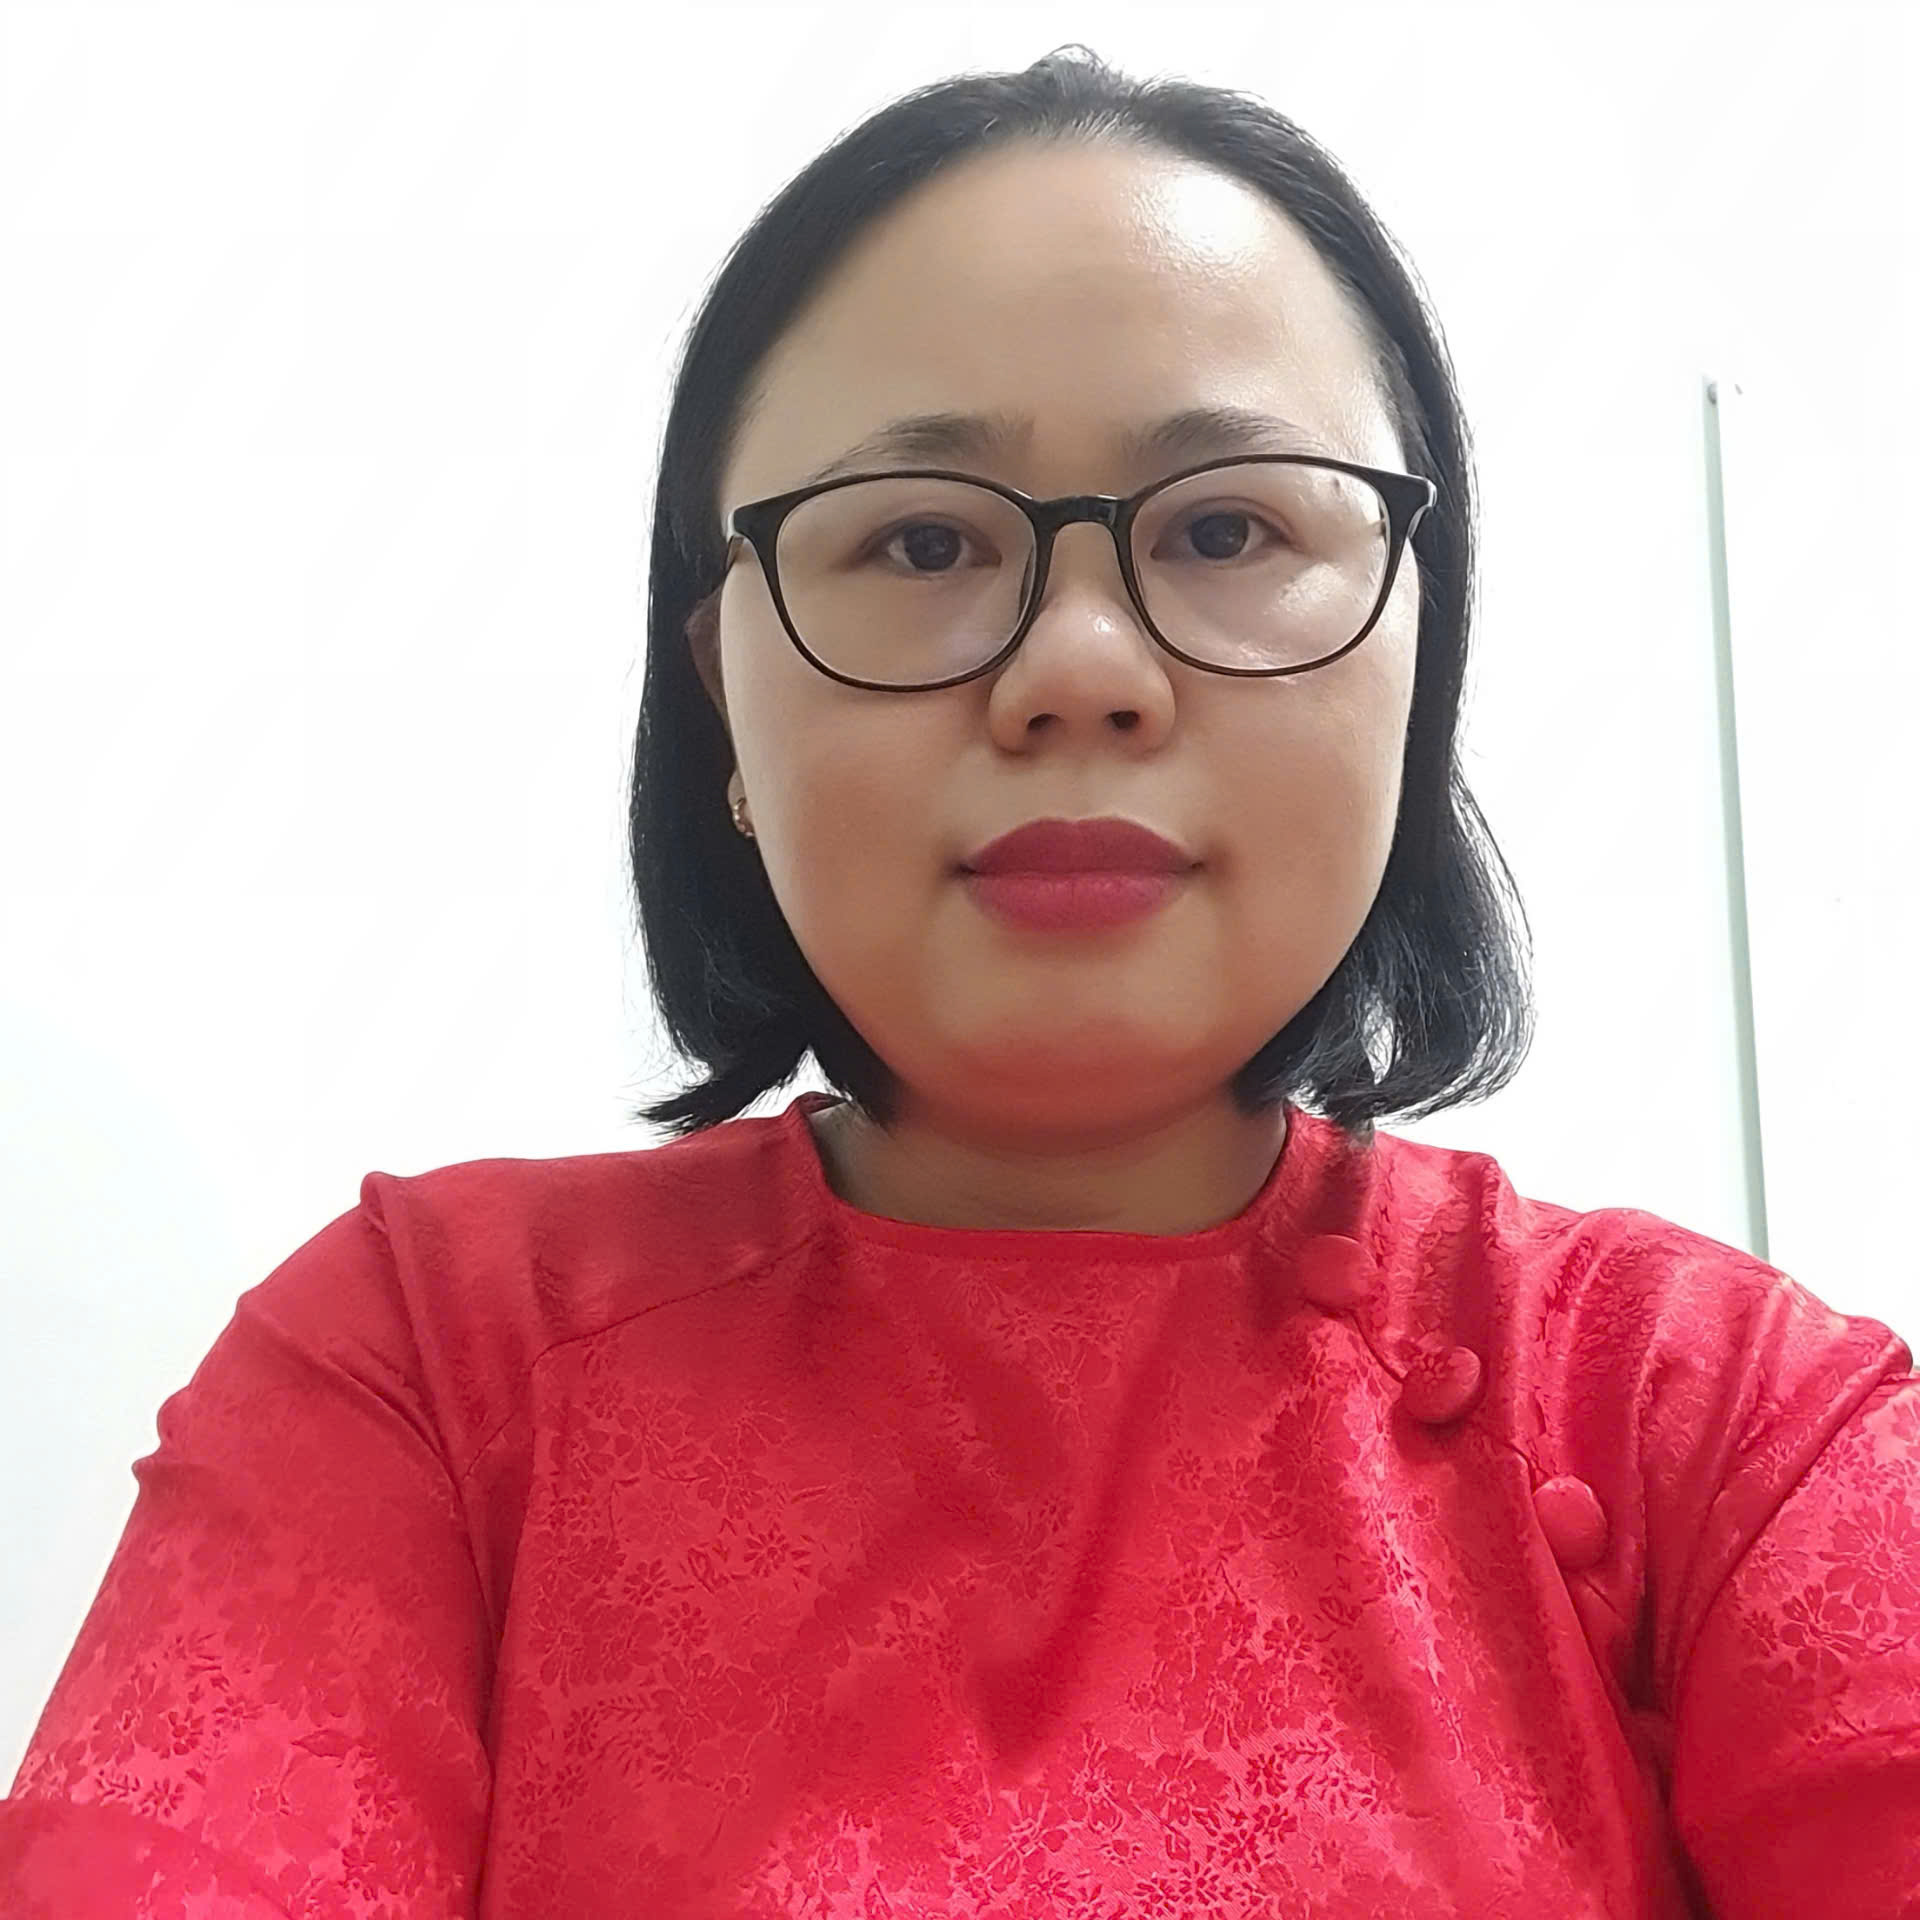
\includegraphics[width=1.0in,height=1.25in,clip,keepaspectratio]{proflie_NguyenNhatHuy.jpg}}]{Nguyen Nhat Huy} received the B.S. degree in Computer Science from Ton Duc Thang University, Ho Chi Minh City, Vietnam, in 2026. His research interests focus on speech and language processing, generative AI, deep reinforcement learning, and combinatorial optimization.
\end{IEEEbiography}

\begin{IEEEbiography}[{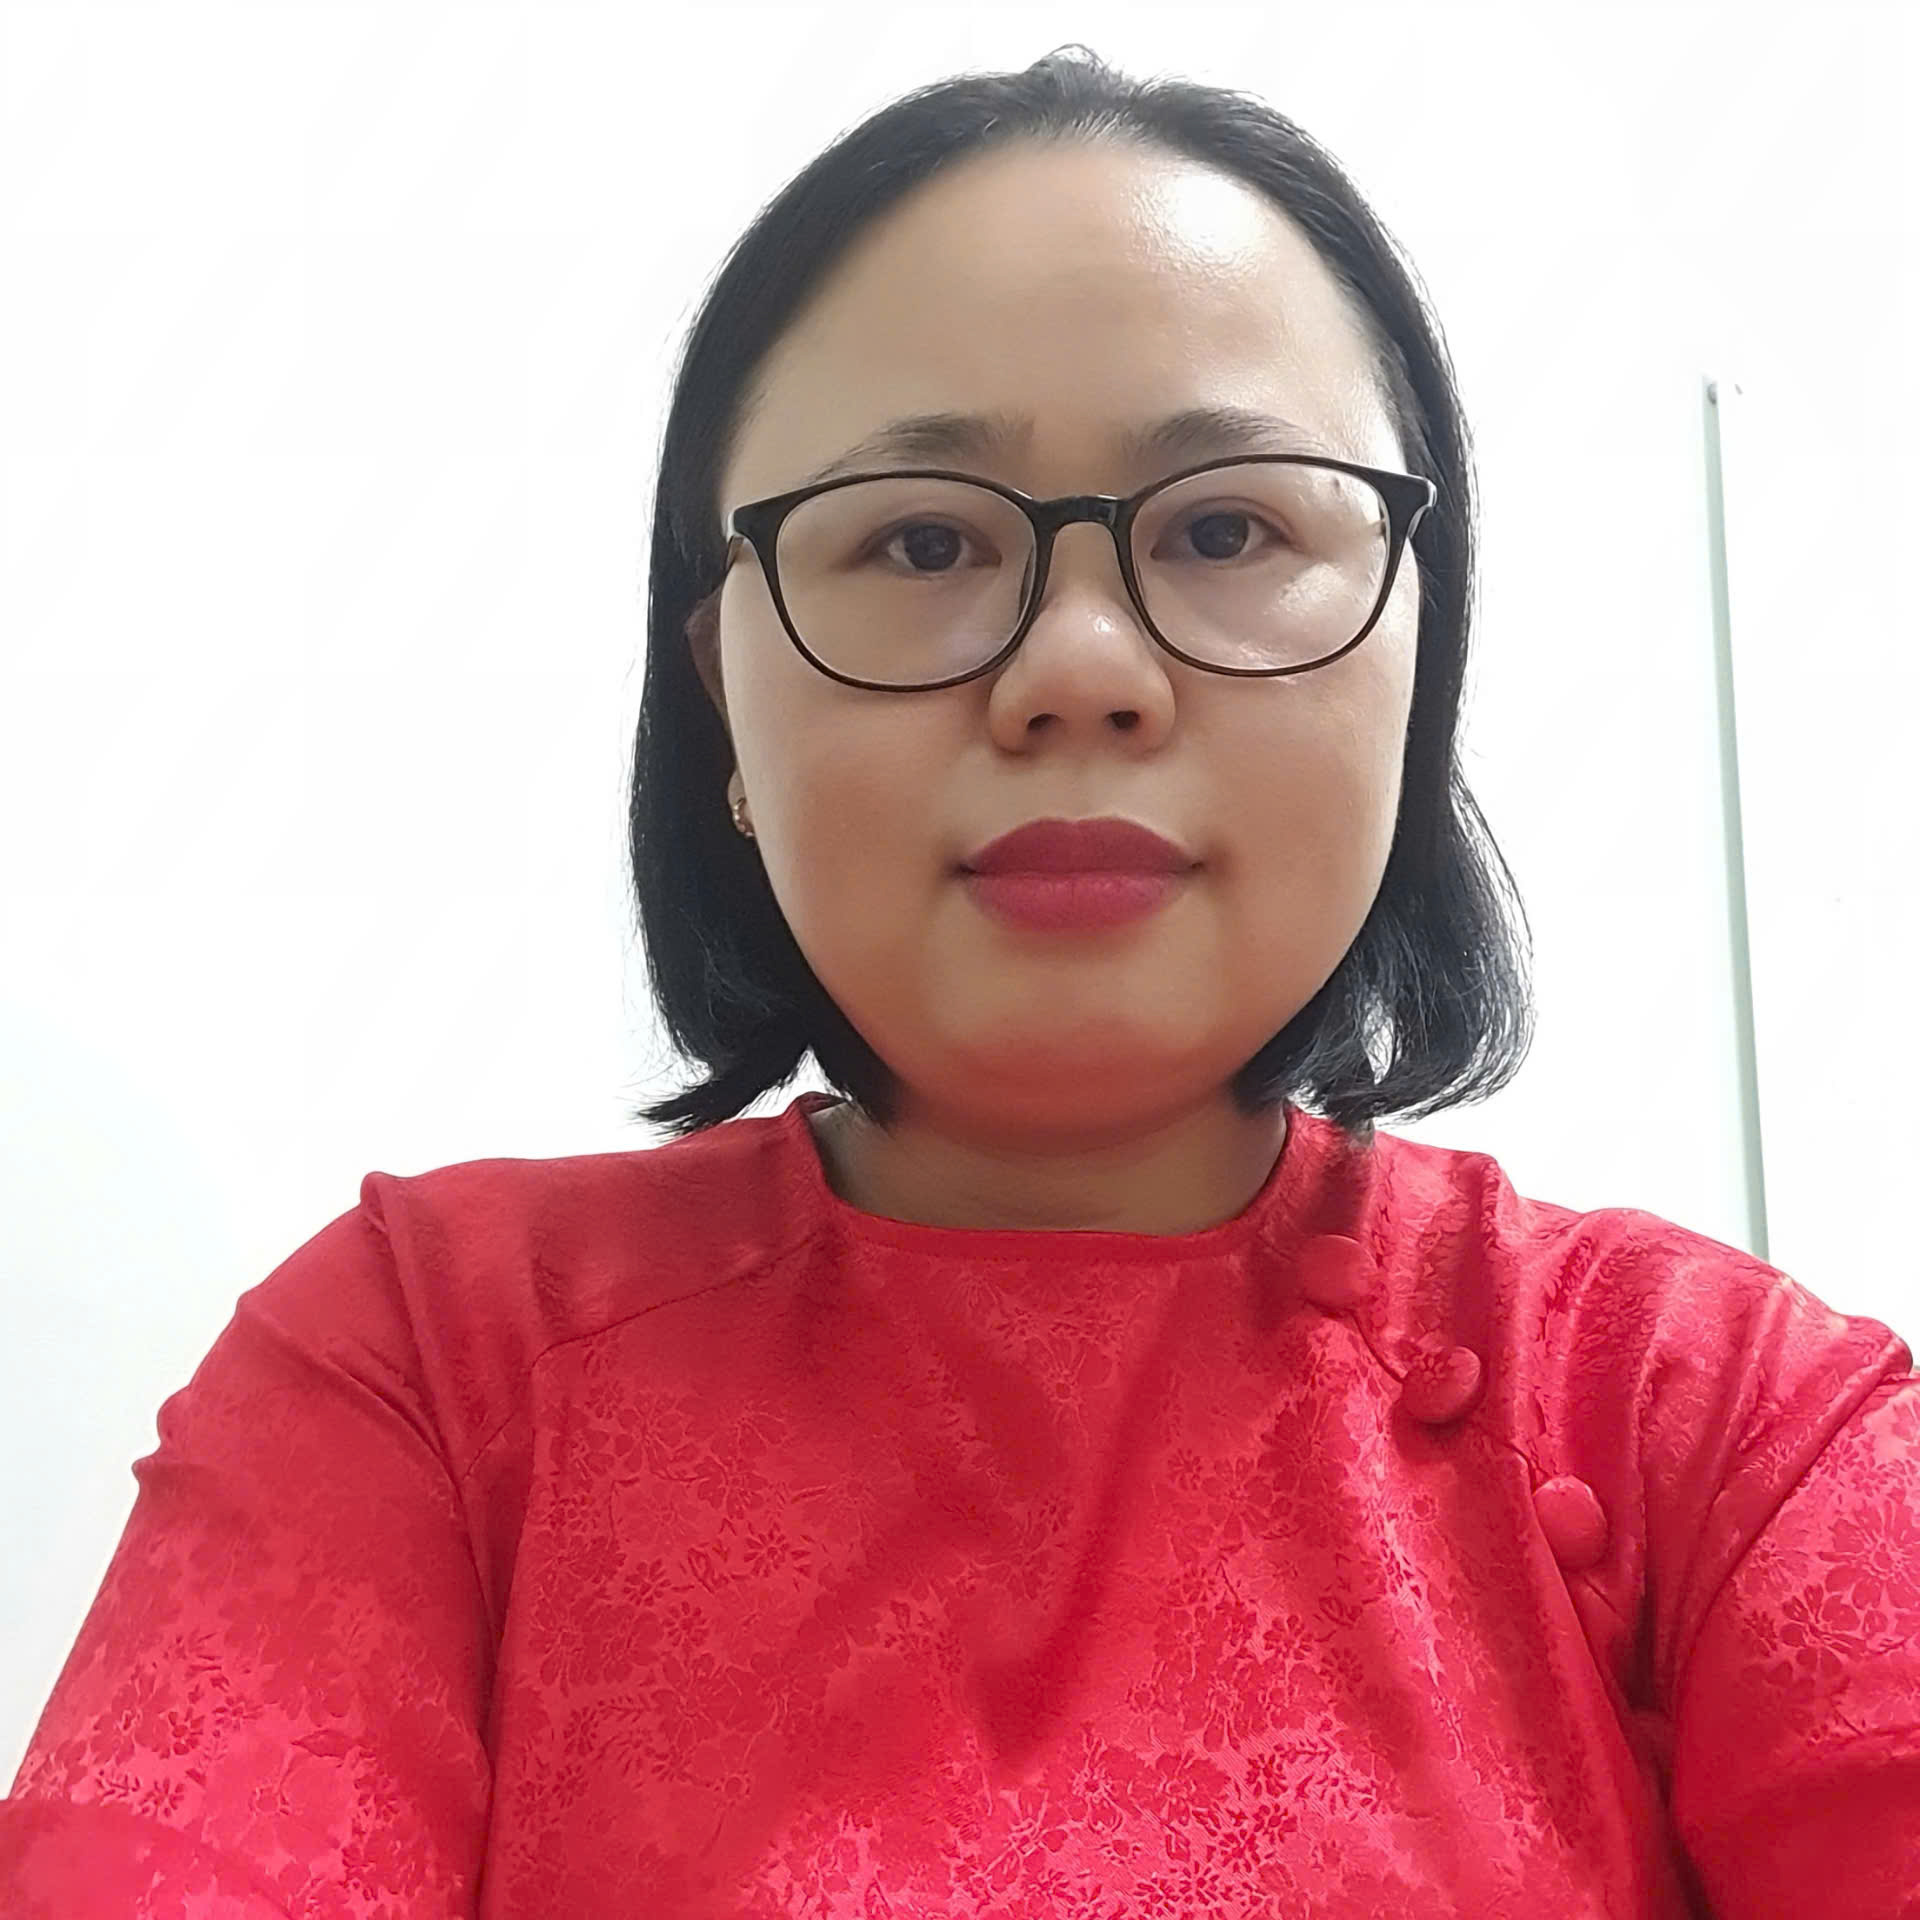
\includegraphics[width=1.0in,height=1.25in,clip,keepaspectratio]{profile_Tran.jpg}}]{Nguyen Thi Bao Tran} received the B.S. degree in Software Engineering from Ton Duc Thang University, Ho Chi Minh City, Vietnam, in 2026. Her current research interests include speech and language processing, generative AI, deep reinforcement learning, and combinatorial optimization.
\end{IEEEbiography}

\EOD

\end{document}
